% !Mode:: "TeX:UTF-8"
%%
%% This is file `thesis.tex',
%% generated with the docstrip utility.
%%
%% The original source files were:
%%
%% chdupaper.dtx  (with options: `thesis')
%%
%% This is a generated file.
%%
%% Copyright (C) 2013 by Tsingber Lee <xiaolee2520@gmail.com>
%%
%% This file may be distributed and/or modified under the
%% conditions of the LaTeX Project Public License, either version 1.0
%% of this license or (at your option) any later version.
%% The latest version of this license is in:
%%
%% http://www.latex-project.org/lppl.txt
%%
%% and version 1.3a or later is part of all distributions of LaTeX
%% version 2004/10/01 or later.
%%
%% To produce the documentation run the original source files ending with `.dtx'
%% through LaTeX.
%%
%% Any Suggestions : Tsingber Lee <xiaolee2520@gmail.com>
%% Thanks LiuBenYuan <liubenyuan@gmail.com> for the NUDT paper!
%%
%3. 如果使用是Vista
% \documentclass[bachelor,ttf,vista]{chdpaper}
%4. 建议使用OTF字体获得较好的页面显示效果
%   OTF字体从网上获得,各个系统名称统一,不用加vista选项
%   如果你下载的是最新的(1201)OTF英文字体,建议修改chdupaper.cls,使用
%   Times New Roman PS Std,但是在该版本中参考文献目标引用会出现问题
%5. 如果想生成盲评,传递anon即可,仍需修改个人成果部分
% \documentclass[bachelor,otf,anon]{chdpaper}
%
\documentclass[bachelor,otf,showtypeinfo,thesis]{chdpaper}%不要模板信息页,可以去掉showtypeinfo选项
%%draftt只加水印,而draft不插图和代码,没有超链接,没有书签
\usepackage{mychd}
\title{Chdpaper宏包XeLaTeX模板使用手册}{\Chdpaper{}宏包\XeLaTeX{}模板使用手册}%论文题目
\school{信息工程学院}%学院
\subject{电子信息工程}%专业
\author{Tsingber Lee}%作者
\Class{24000900}%班级
\serialno{2400090001}%学号
\supervisor{$\mathbb{C}$\TeX{}}
\endate{\entoday}%可以手动填写日期
\zhdate{\zhtoday}
%%任务开始结束日期
\tbmonth{3}%月
\tbday{1}%日至
\temonth{6}%月
\teday{10}%日共
\totalweeks{15}%周
\begin{document}
\graphicspath{{figures/}}%图片路径
% 制作封面,任务书及开题报告,生成目录,插入摘要
\maketitle%注释掉此行,可以不生成此封面,任务书及开题报告。一起由word转为pdf,由下面载入
%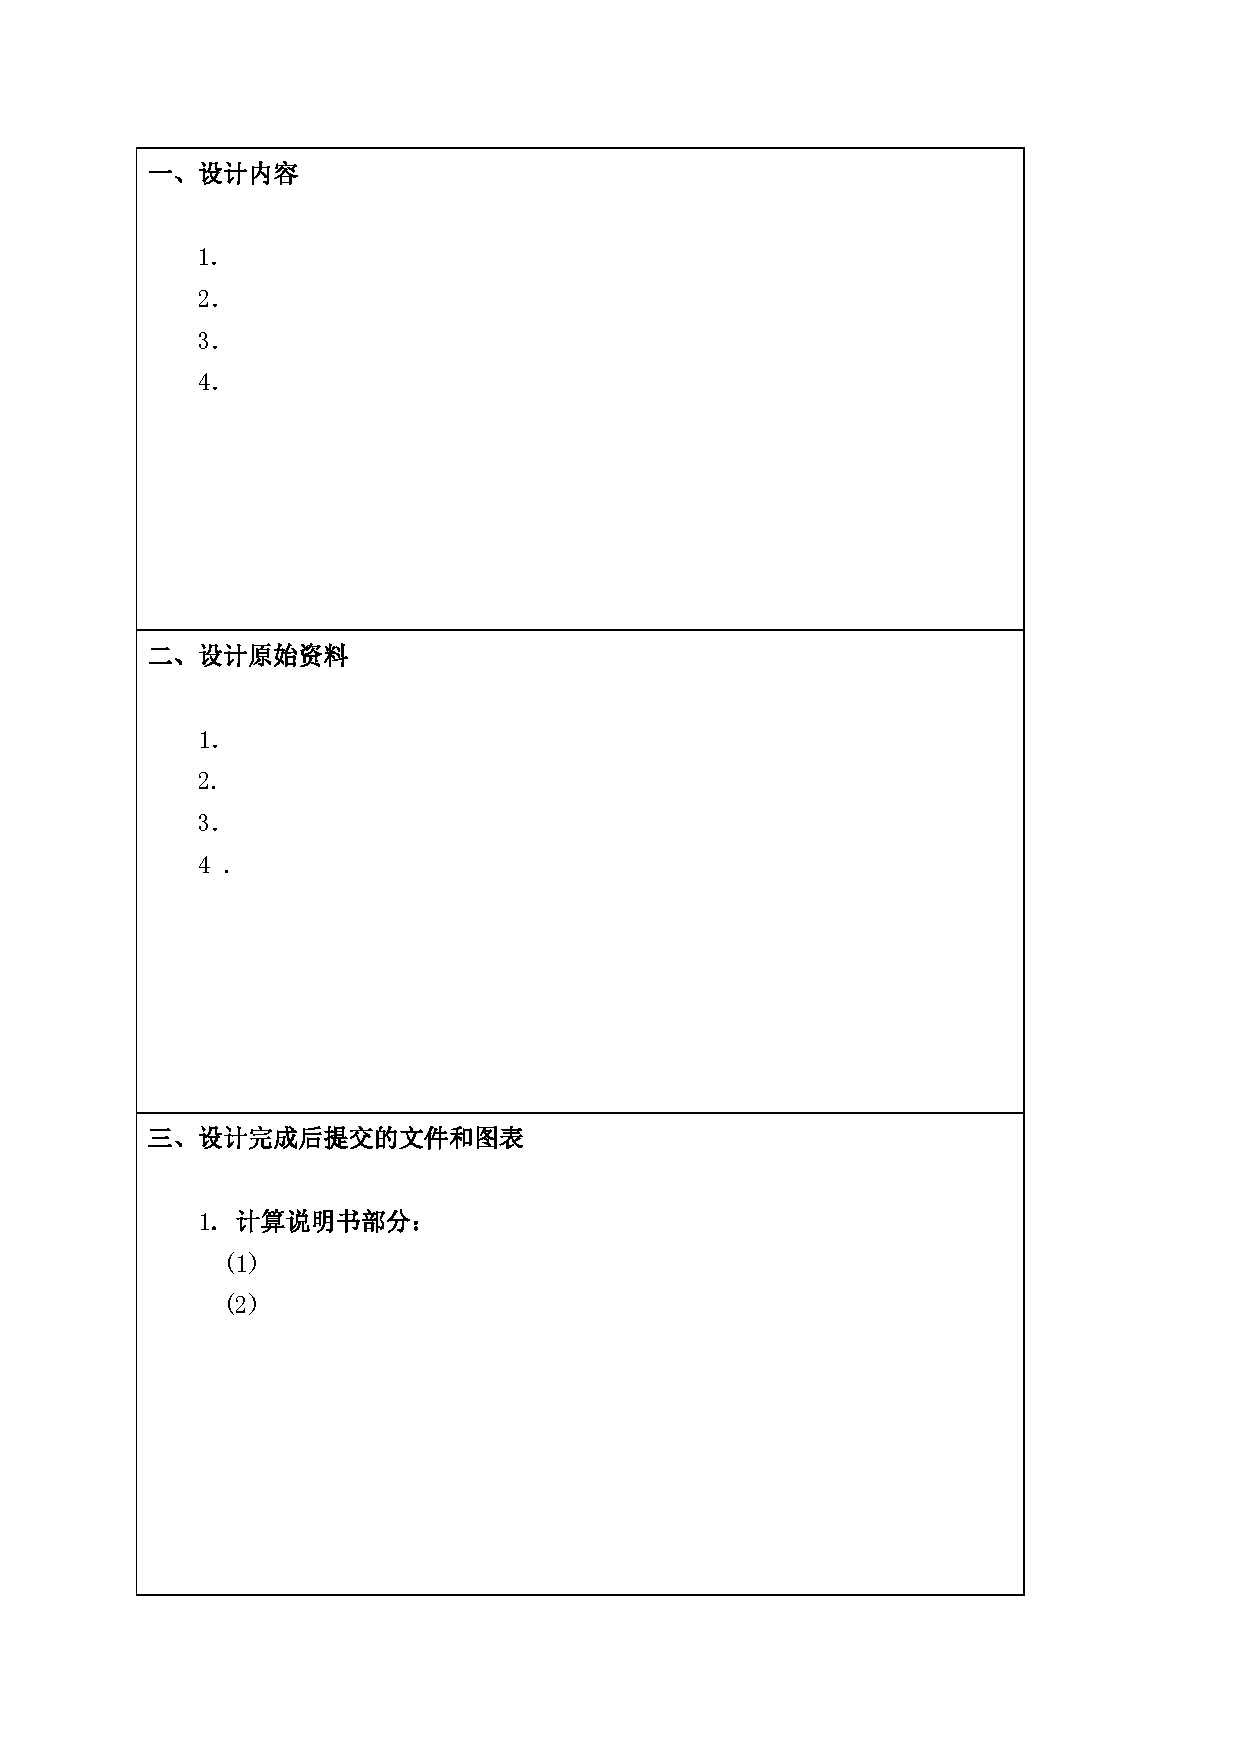
\includepdf[nup=1x1, delta=0mm 0mm,scale=1,pages={1-5}]{a3cover/frontpage.pdf}
%
\frontmatter
% !Mode:: "TeX:UTF-8"
\begin{cabstract}
\TeX{}是一个排版系统,可以把文章做成书那种效果。因此\TeX{}非常适合用来写学术论文和书籍。\chdpaper{}是按照长安大学教务处对本科生毕业论文的要求设计和实现的\LaTeX{}模板,帮助长安大学的学生以专业排版水平来完成毕业论文。

本文既是\chdpaper{}使用手册也是范例,建议在使用\chdpaper{}之前阅读。

长安大学直属国家教育部,是教育部、交通运输部、住房和城乡建设部、国土资源部和陕西省政府共建的国家“211工程”重点建设大学,是国家“985工程”优势学科创新平台建设高校。

长安大学2000年是由始建于二十世纪50年代初的原西安公路交通大学、西安工程学院、西北建筑工程学院合并组建而成,是一所以工为主,理工结合,经济、管理、人文多种学科协调发展,以培养公路交通、国土资源与环境、建筑工程等专业人才为办学特色,在国内外有很大影响的高等学府。
\end{cabstract}
\ckeywords{长安大学,211,长大}
\newpage
\begin{eabstract}
\TeX{} is a typesetting system, it can make article as good as {\em published book}. Therefore, \TeX{} is very suitable for writing academic papers and books. \chdpaper{}is designed and implemented as a \LaTeX{} template to help studnets writing degree thesis in a professional typesetting, according to the requirements of Chang'an University.

This paper is \chdpaper{}user manual and also the sample document, it is better to be read before using \chdpaper{}.

Chang'an  University is a comprehensive national key university based in Xi'an, %
Shaanxi Province, China. It is under the dual supervision of the State Education Department, Ministry of land and resouces and the government of Shaanxi province, designated for Project 211, %
the plan for facilitating the development of Chinese higher education. %

CHD was founded in 2000 with the merger of original Xi'an Highway University,Xi'an College of Engineering,Northwestern Institude of Architectural Engineering which were founded at the beginning of the 50's in twentieth Century. %
To cultivate professional talents of highway traffic,land resoureces and environment,construction engineering as school characteristics,Chang'an  University is an institutions of higher learning that has great influnce in the domestic and foreign.
\end{eabstract}
\ekeywords{211, CHD, Chang'an  University}
\newpage%中英文摘要
\pdfbookmark[0]{目~~录}{mulu}
\tableofcontents%目录
%书写正文,可以根据需要增添章节; 正文还包括致谢,参考文献与成果
\mainmatter
% !Mode:: "TeX:UTF-8"
\chapter{引言}
\mingyan{满纸荒唐言,一把辛酸泪!都云作者痴,谁解其中味?}{曹雪芹}

本模板完全由国防科技大学的模板改来,初次制作,不足之处在所难免,欢迎提供建议,在此感谢Liubenyuan同学,模板里很多地方对我帮助很大。模板详细说明基本上可以参考nudtpaper-2.2.pdf。

我还是比较满意我做的两个封面\footnote{论文封面和任务书封面},你只需在thesis.tex中仿照模板填上相关数据即可。由于我们学校的论文要求里面也没说正文版面大小,我就根据以前一个学姐的论文测量出页边距,页眉,页脚等一些参数,做的这个。算是基本满足学校的要求了,就看学校收不收了。
\section{本模板的一些使用说明}
任务书及开题报告本来是不想做的,有些难度。但真是皇天不负有心人,终于让我在天津大学的模板里找到了这个东西,花了一个下午做出了那些表格。当然你也可以不用我做的那个,将\verb|% !Mode:: "TeX:UTF-8"
\pagestyle{empty}
\vspace*{1ex}
\myoverlay%为当前页添加边框
{\cusong\sihao\hspace*{-2em} 一、设计内容}
     \begin{enumerate}
     \item 准备了解有关导航以及导航系统的特点、应用前景。
     \item 准备对导航系统中常用的惯导器件—陀螺仪进行说明。
     \item 准备对提高导航信号测量精度所用到的滤波技术进行软件仿真。
     \item 准备分析比较各种滤波信号,并得出相应结论。
     \end{enumerate}

\myhline%划横线
{\cusong\sihao 二、设计原始资料}
     \begin{enumerate}
     \item 导航系统的相关资料
     \item 惯导器件基础教程及有关书籍
     \item 卡尔曼滤波、神经网络相关资料
     \item \Matlab{}软件教程及相关资料
     \end{enumerate}

\myhline%划横线
{\cusong\sihao 三、设计完成后提交的文件和图表}
     \begin{enumerate}
     \item 计算说明书部分
     \begin{enumerate}
     \item 卡尔曼滤波、扩展卡尔曼滤波以及无迹卡尔曼滤波对比仿真图
     \item 各种滤波算法应用范围对比表
     \end{enumerate}
     \item 图纸部分
     \begin{enumerate}
     \item 几种惯性导航系统原理框图
     \item 改进卡尔曼滤波效果仿真图
     \item 卡尔曼滤波、扩展卡尔曼滤波以及无迹卡尔曼滤波效果仿真比较图
     \end{enumerate}
     \end{enumerate}

\myhline
{\cusong\sihao 四、毕业设计进程安排}

          \vspace{2em}
          {\heiti 序号\hspace{5em}设计各阶段名称\hspace{9em}日期(教学周)}

          {\hspace{0.5em}1\hspace{3em}阅读相关书籍,完成开题报告\hspace{4em}3月1 日--3月14日(第1--2周)}

          {\hspace{0.5em}2\hspace{3em}准备了解常见导航系统的相关知识\hspace{2em}3月15 日--3月28日(第3--4周)}

           {\hspace{0.5em}3\hspace{3em}研究导航系统中较常见的惯导器件\hspace{2em}3月29日--4月11日(第5--6周)}

           {\hspace{0.5em}4\hspace{3em}学习导航系统中几种常用滤波技术\hspace{2em}4月12日--5月9日(第7--10周)}

           {\hspace{0.5em}5\hspace{3em}准备对滤波算法进行仿真比较\hspace{4em}5月10日--5月16日(第11周)}

           {\hspace{0.5em}6\hspace{3em}撰写毕业论文\hspace{11em}5月17日--6月10日(第12--14周)}

\myhline
{\cusong\sihao 五、主要参考资料}
\begin{bibList}
\item 于国强. 导航与定位. 北京:国防工业出版社.2000.2:1.
\item 邓正隆. 惯性导航原理.哈尔滨:哈尔滨工业大学出版社.1994.1:1-2,2-5.
\item 袁建平. 卫星导航原理与应用.中国宇航出版社.2003 第一版:23-24.
\item 秦永元. 惯性导航.北京:中国科学出版社.2006:1-5.
\item 陈开权. 惯性导航的理论基础[J]. 北京: 水雷战与舰船防护,2003(1):76-90.
\item 付梦印,邓志红,张继伟.Kalman 滤波理论及其在导航中的应用.北京:科学出版社.2003.
\end{bibList}

%%%%%%%%%%%%%%%%%%%  长安大学毕业设计(论文)开题报告表  %%%%%%%%%%%%%%%%%%%%%%%
\newpage
\markboth{长安大学毕业设计(论文)开题报告表}{长安大学毕业设计(论文)开题报告表}
\pdfbookmark[0]{长安大学毕业设计(论文)开题报告表}{creport}
\begin{center}
\hei\sanhao{长安大学毕业设计(论文)开题报告表}
\end{center}
\begin{table}[h]
  \centering\xiaosi
  \begin{tabularx}{\textwidth}{|c|p{0.15\textwidth}|c|X|c|X|}
     \hline
     课题名称 & \multicolumn{5}{c|}{TeX惯性器件精度提高实现方法} \\ \hline
     课题来源 & \centering {自选课题} & 课题类型 & \centering {工程设计} & 指导教师 & \centering {CTeX} \tabularnewline \hline
     学生姓名 & \centering {Tsingber  Lee} & 学\hspace*{24bp}号 & \centering {2403000001} & 专\hspace*{24bp}业 & \centering {电子信息工程} \tabularnewline \hline
   \end{tabularx}
      \centering\xiaosi
\end{table}
%%%%%%%%%%%%%%%%%画图区%%%%%%%%%%%%%%%%%
\setlength{\unitlength}{1mm}
\noindent\begin{picture}(0.1,0)
\multiput(0.1,0)(160.8,0){2}{\line(0,-1){188}}
\multiput(0.1,0)(160.8,0){2}{\line(0,1){9.3}}
\put(0.1,-188){\line(1,0){160.8}}
\end{picture}
%%%%%%%%%%%%%%%%%%%%%%%%%%%%%%%%%%
     {  {\heiti (一)课题意义:}

 由半导体工业中的微细加工技术与机械工业中的微型机械加工技术结合而产生并逐渐发展起来的微电子机械系统(MEMS: Microelectro Mechanical Sys2tem) 是微米、纳米电子学的重要领域,是一项极具发展前景的军民两用高技术,它的出现,将引发一场新的技术革命。

微电子机械系统涉及到微电子学、自动控制、光学、气动力学、流体力学和声学磁学等多种领域,可以说是一门多学科的综合技术。它研究的主要内容包括微型传感器、微型执行器和复杂的微系统。提高MEMS加速计传感器的精度具有重要意义。

{\noindent\heiti (二)国内外发展状况:}

(1)国外概况:

MEMS 技术的开发始于20 世纪60 年代,其迅速发展是在20世纪80年代末期,由MEMS技术的迅速发展,在1987年便决定把MEMS从IEEE国际微机器人与过程操作年会分开,单独召开年会。目前每年在美、日、欧三地轮回举行名为IEEE 国际MEMS年会(Microelectro Mechanical Systems Workshop ) 。

美国是研究开发MEMS最早的国家,早在上世纪60年代加利福尼亚大学和贝尔实验室就开始这方面的研究,曾开发出微型硅压力传感器,后又在20世纪70年代开发出硅片色谱仪、微型继电器。特别是在20世纪90年代初,加大利用“牺牲层”技术,制造出一台直径小于人发的超微静电电动机,曾在世界引起很大轰动,专家纷纷预测其广阔的应用前景。此后,美国超微机电系统的研究走上有序开发阶段,取得了一系列被专家称为具有划时代意义的成果。

1987年,美国加州大学Berekeley分校的范龙生等人在第四届国际固态传感器与执行器会议上,报道了用表面微机械加工技术制作的多晶硅齿轮,引起了世界各国科学家的注意,此后微电子机械系统工程成为人们关注的新兴学科。LIGA 技术是在20世纪80年代中期由德国Karlsruhe原子核研究中心发展起来的,包括同步辐射深度光刻、微电铸、微塑铸3个过程。
目前全世界研制生产MEMS有600多个单位,已研究出几百种产品,其中微电子传感器占大部分。


     (2)国内概况:

我国开展MEMS 研究始于20世纪80年代末,10多年来研究队伍迅速发展和扩大,目前已有40多个单位的50多个研究小组,在新原理微器件、通用微器件、新的工艺和测试技术以及初步应用等方面取得了显著的进展。

1995年国家科技部实施了攀登计划“微电子机械系统项目”(1995~1999 年) 。1999年“集成微光机电系统研究”项目通过了国家重点基础研究发展规划的立项建议。我国已开展了包括微型直升飞机、力平衡加速度传感器、力平衡真空传感器、微泵、微喷嘴、微电机、微电泳芯片、微流量计、硅电容式麦克风、分裂漏磁场传感器、集成压力传感器、微谐振器和微陀螺等许多微机械器件的研究和开发工作。研究出的硅电容式微麦克风是目前国际同类研究中灵敏度最高的;在国际上首次研制出包括片上转速检测电路的集成硅微静电电机;分裂漏磁场传感器、集成压力传感器、硅微静电电机工艺已取得三项美国专利。

我国的MEMS研究已经历了10多年的发展,虽然有一些器件和机构被研制出来,但目前整体仍处于基础性阶段,极少有实用的MEMS器件。与国际上的最大差别是在产业化推进方面尚未具备大批量生产的能力。为此,我们应该根据MEMS器件制造的特点,从工艺研究入手,对一些有一定研究基础、应用面广、市场前景好的MEMS产品,进行重点攻关,掌握成熟的制造工艺,为产业化推进铺平道路。

{\noindent\heiti (三)本课题的研究内容:}

MEMS惯性器件存在测量精度低、噪声大等缺点,需要采取一些必要的措施以提高其精度,除了优化机械结构设计,提高电子线路的性能,以及采取屏蔽外部电磁干扰措施之外,另一种有效的途径是:从应用的角度对MEMS惯性器件和微惯性测量单元(MIMU)进行误差分析及补偿,提高系统的测量精度。本课题在主要通过改进滤波器来提高其精度,内容有:

1.首先对导航技术中几个主要惯性器件进行初步介绍

2.对于导航技术中应用十分广泛的几种滤波技术进行了比较深入地研究

3.通过神经网络等技术对其进行初步改进

{\noindent\heiti (四)本课题的研究方法:}

首先介绍几种常见的导航系统,之后对应用最为广泛的惯性导航系统所使用的滤波技术进行了深入研究说明,并提出自己的改进方法。最后编写相应程序以测试方法的优缺点。

\myoverlay%为当前页添加边框

{\noindent\heiti (五)本课题的研究手段:}

阅读有关MEMS导航系统相关资料,对导航理论有一个基本的了解,在些基础上,对相关的滤波算法进行一定的学习与比较,了解算法的基本原理和思想。使用Matlab软件编程,对滤波器进行仿真对比。	

{\noindent\heiti (六)本课题的研究成果:}

本报告通过Matlab仿真比较得出最为有效、滤波效果最佳的滤波方法。

     {\noindent\heiti (七)任务完成的阶段安排及时间安排:}

(1)3月1日-3月14日(第1-2周)

阅读相关书籍,完成开题报告。

(2)3月15日-3月28日(第3-4周)

学习导航系统,对常见的导航系统有所了解。

(3)3月29日-4月11日(第5-6周)

研究导航系统中常用的惯导器件,对其中较为关键的惯导器件—陀螺仪有比较清楚地认识。

(4)4月12日- 5月9日(第7-10周)

对导航系统中涉及的滤波技术以及神经网络技术作深入学习,了解它们的特点。

(5)5月10日-5月16日(第11周)

对各种滤波算法进行仿真比较。

\myoverlay%为当前页添加边框
\myoverlay%为当前页添加边框
(6)5月17日- 6月8日(第12-14周)

撰写毕业设计论文

(7)6月9日-6月17日(第15周)

提交论文评审与答辩

     {\heiti (八)任务所具备的条件因素:}\myoverlay

(1)对导航及导航技术有初步了解。

(2)了解并清楚常见导航系统之间的优缺点,知道它们的应用前景。

(3)熟悉导航滤波技术中各种滤波算法的原理及特点。

(4)能够比较熟练地运用Matlab仿真软件。

\myhline

指导教师意见及建议: \\
     \vfill
     {\hfill 指导教师签名:\hspace*{5cm}}

     \vspace{1em}
     {\hfill 年\hspace*{0.7cm}月\hspace*{0.7cm}日\hspace*{5cm}}\vspace*{1cm}
\thispagestyle{empty}|注释掉。再在word里填好,然后转换为pdf,存储名为frontpage.pdf,放到a3paper文件夹下。并在thesis.tex中找到这句\verb|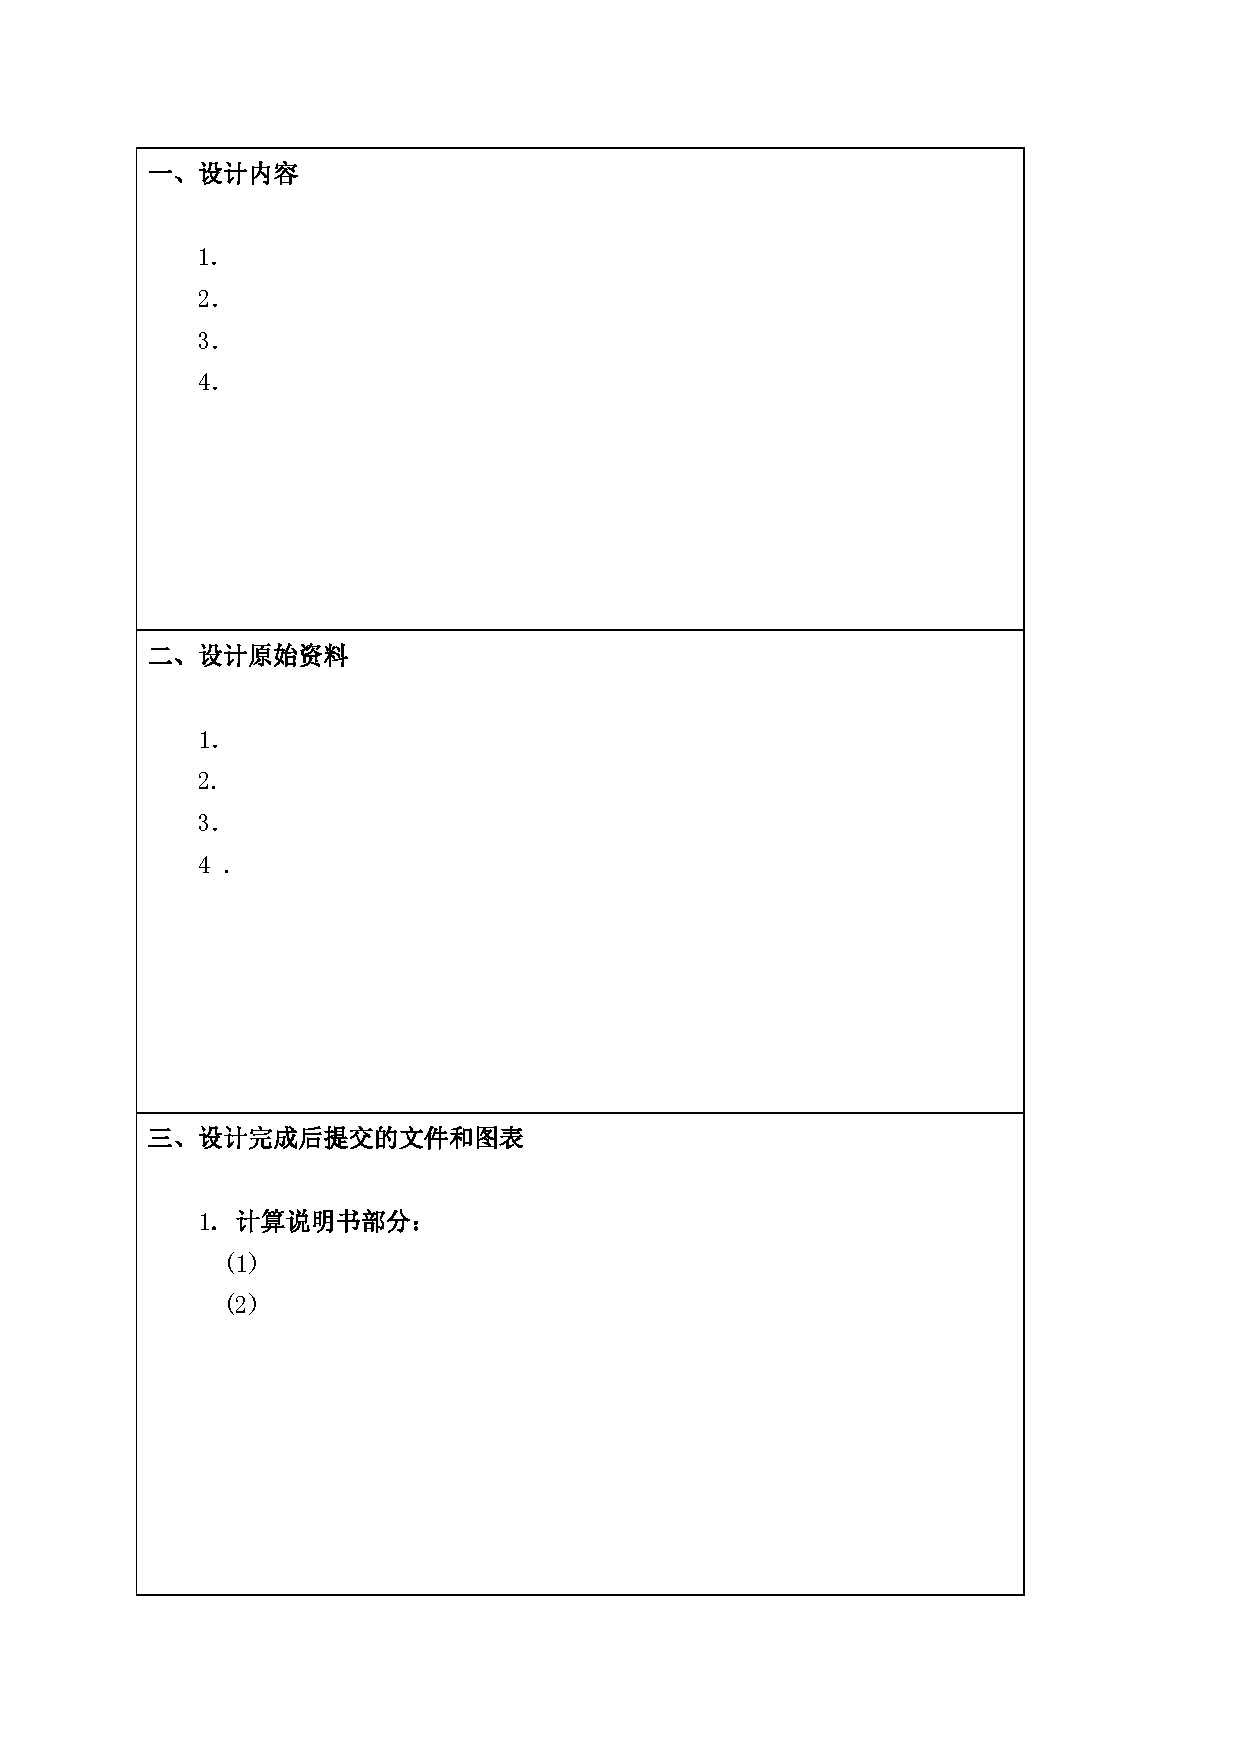
\includepdf[nup=|\verb|1x1, delta=0mm 0mm,scale=1,pages={1-6}]{a3cover/frontpage.pdf}|,其中\verb|pages={1-6}|是你frontpage的页码范围。还有附件里的外文文献及翻译,也是用这种方法载入。还有\LaTeX{}分段缩进不用空格,直接回车两下,就是空一行

像这样,详细参考本文代码。公式、插图、表格下面段落也要空一行,否则不会缩进。但是如果遇见章节标题,就不用空行了,会自动缩进。
\subsection{免责声明}
\begin{myList}
\item 本模板的发布遵守\LaTeX{} Project Public License,使用前请认真阅读协议内容
\item 本模板的出发点是方便大家使用专业的高效的论文书写工具,其优点在于注重排版质量、命令规范、使用方便,符合论文撰写说明。但任何由于使用本模板而引起的论文格式审查问题均与本模板作者无关。
\item 任何个人或组织均可以本模板为基础进行修改、扩展,生成新的专用模板,但
请严格遵守\LaTeX{} Project Public License 协议
\end{myList}
\begin{figure}[htp]
\centering
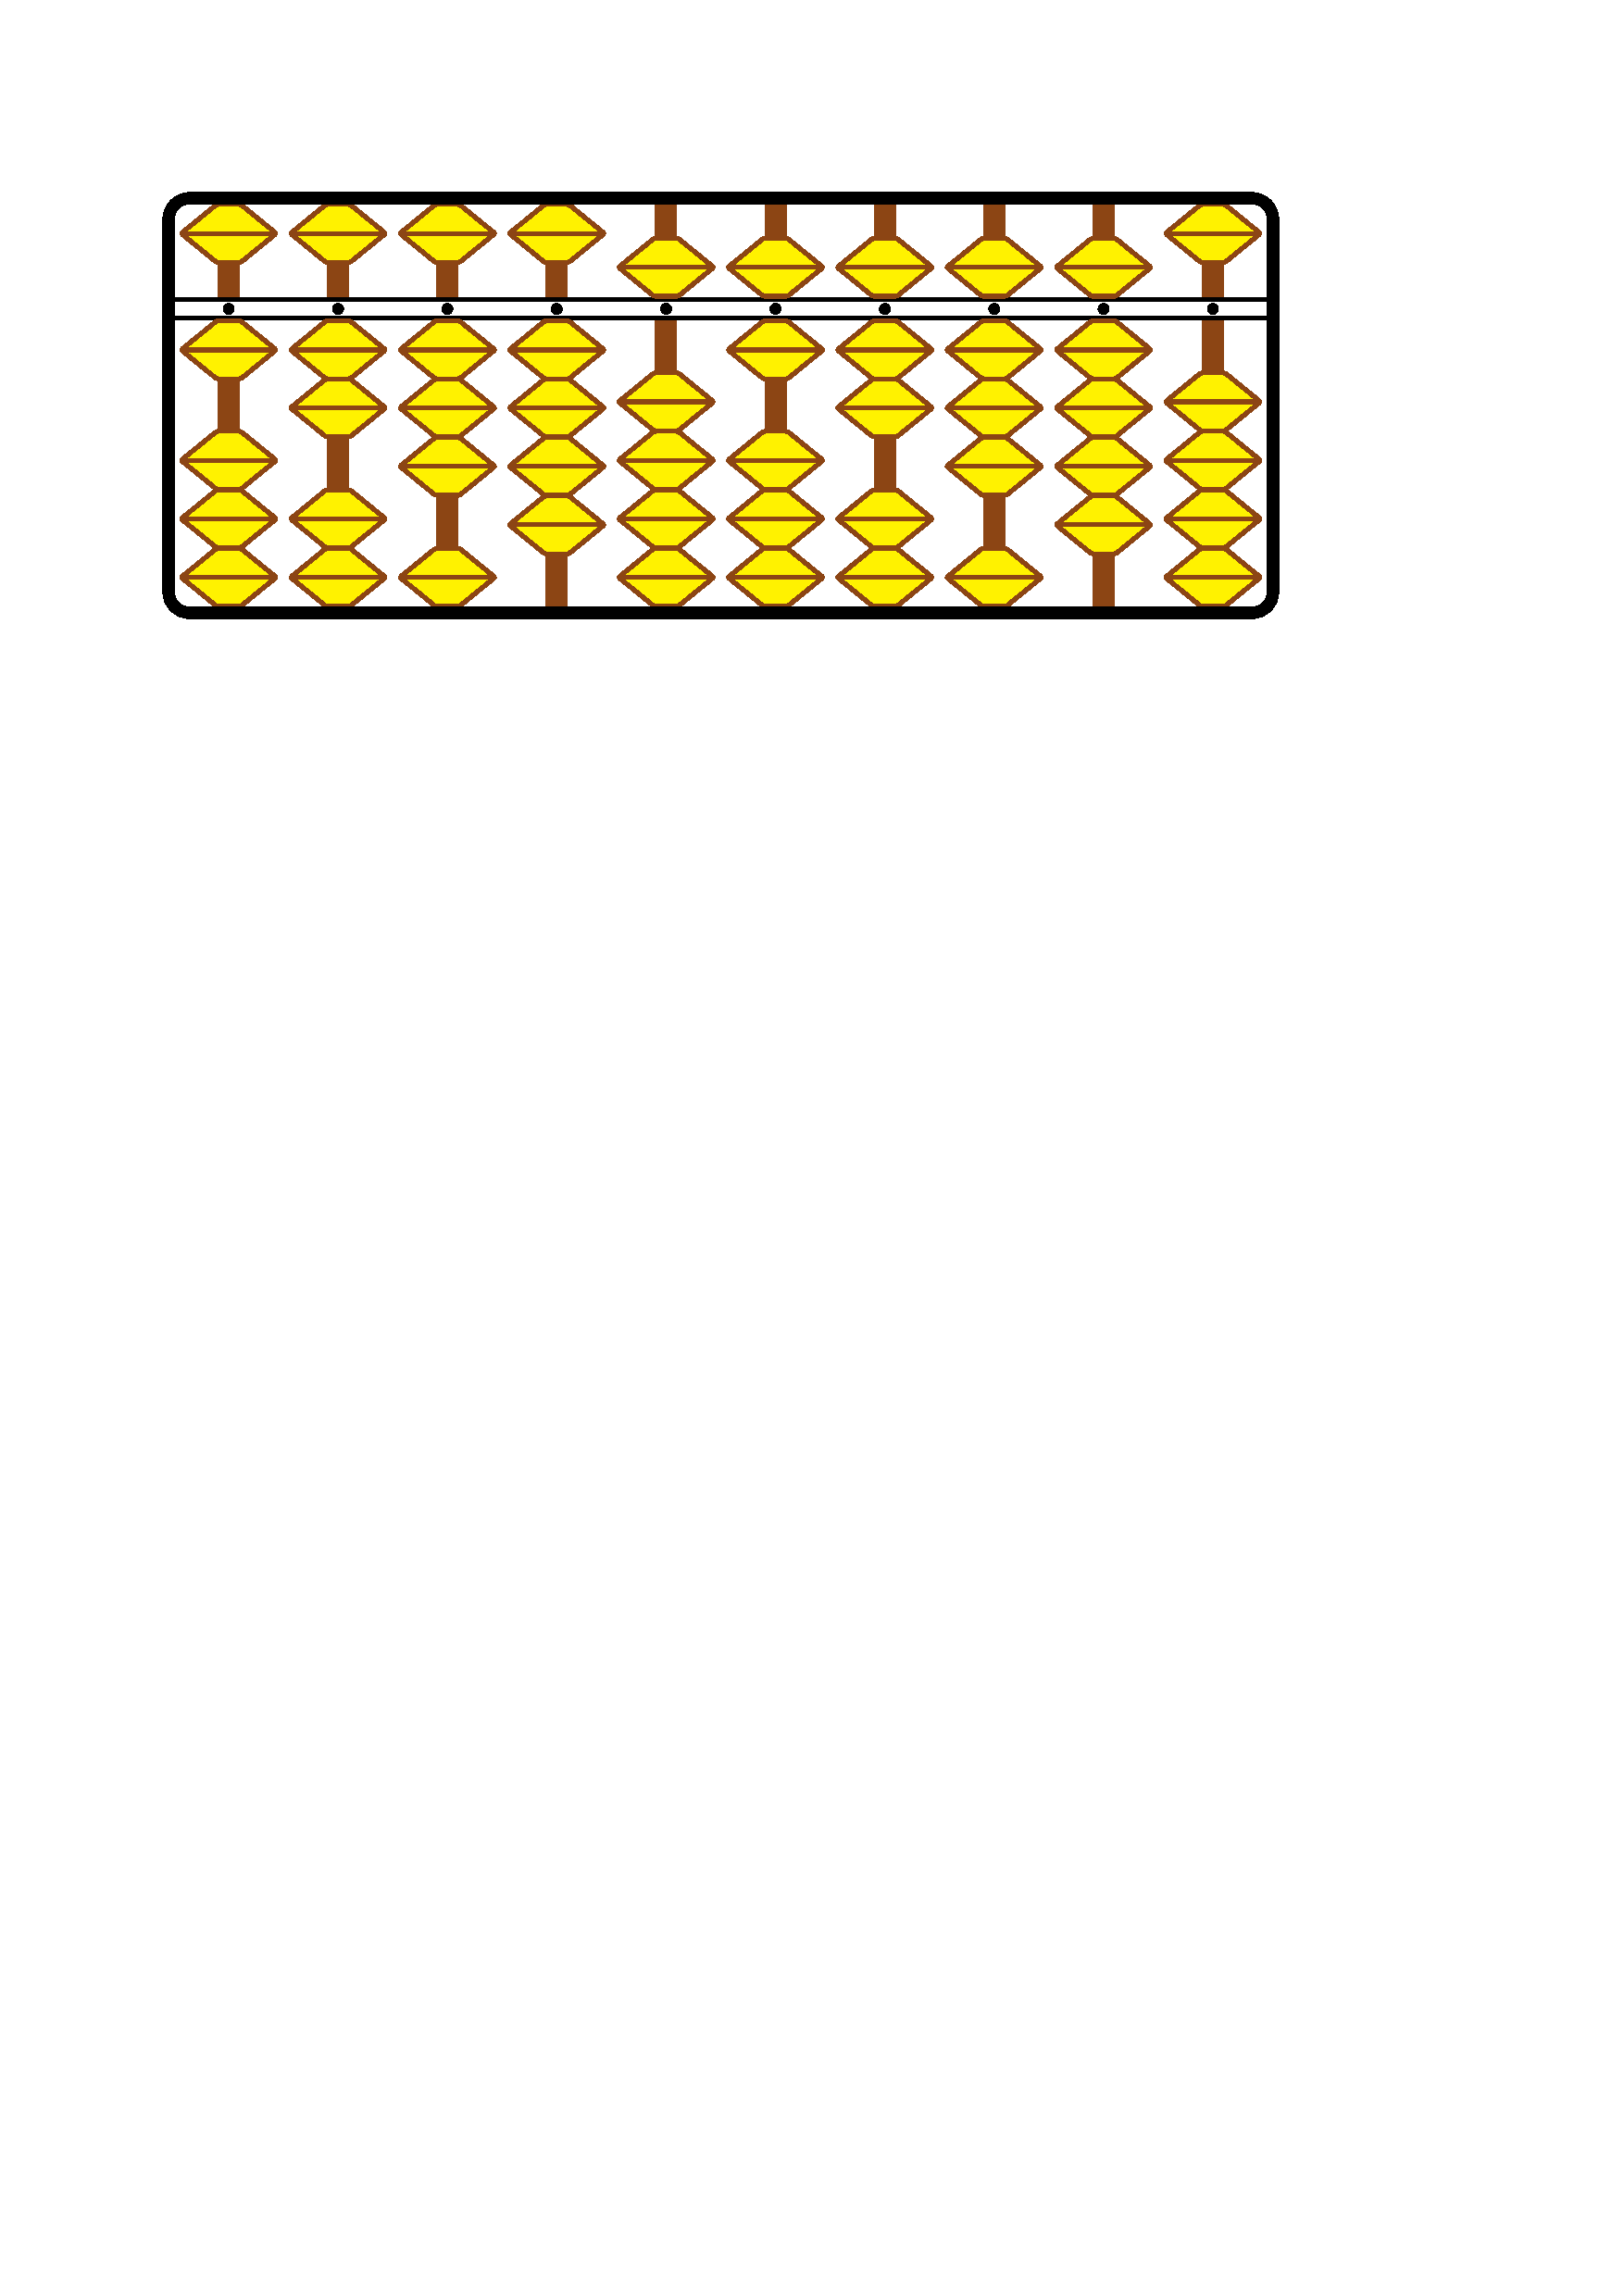
\includegraphics[width=5in]{soroban.pdf}
\caption{soroban宏包绘制的算盘}
\end{figure}

由于有些地方用\verb|itemize|不太合适,也用不上\verb|\subsubsection|这样的小小节,所以就把它改成下面的样子了。但是在每次使用前得先把计数器初始化为1,\verb|\setcounter|\verb|{shuzi}{1}|
\subsubsection{(题目(1))}
本章的主要内容与学校提供的Word模板中内容一致,图片与表格均采用原始设定大小,%
主要是为了说明格式的统一。%
但是,\LaTeX{}的一些禁则,专业排版的能力,对公式及文献的处理都是得天独厚的,%
我们不必刻意去追求与Word的完美匹配。而且你将会发现,用\LaTeX{}书写论文的美! %

\subsubsection{(题目(1))}
用户在使用中遇到问题或者需要增加某种功能,都可以和作者联系:
Tsingber Lee <xiaolee2520@gmail.com>
欢迎大家反馈自己的使用情况,能为长大本科生的作出一点点的贡献,也祝
长安大学的同学前程似锦。

\subsection{(1.1.2 题目)}
正文内容

正文内容
\begin{figure}[htp]
\centering
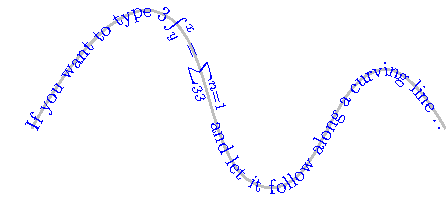
\includegraphics{followline.pdf}
\caption{followline}
\end{figure}

\begin{figure}[htp]
\centering
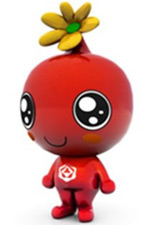
\includegraphics{shiliu.jpg}
\caption{世园会吉祥物}
\end{figure}

\section{1.2节题目}
正文内容

正文内容

\begin{table}[htp]
\centering
\caption{表 1.2 名称}
\begin{tabular}{|c|c|c|c|c|}
\hline
\makebox[2.07cm][0pt]{} & \makebox[2.07cm][0pt]{} & \makebox[2.07cm][0pt]{} & \makebox[2.07cm][0pt]{} & \makebox[2.07cm][0pt]{} \\
\hline
 & & & & \\
\hline
 & & & & \\
\hline
\end{tabular}
\end{table}
\subsection{题目}
\begin{figure}[htp]
\centering
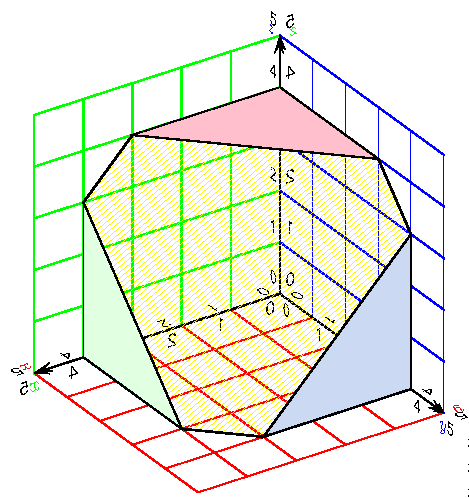
\includegraphics[width=5in]{pstricks-doc1.pdf}
\caption{空间立体}
\end{figure}
\subsection{题目}
正文内容

正文内容

\section{本文主要研究内容}
\begin{figure}[htp]
\centering
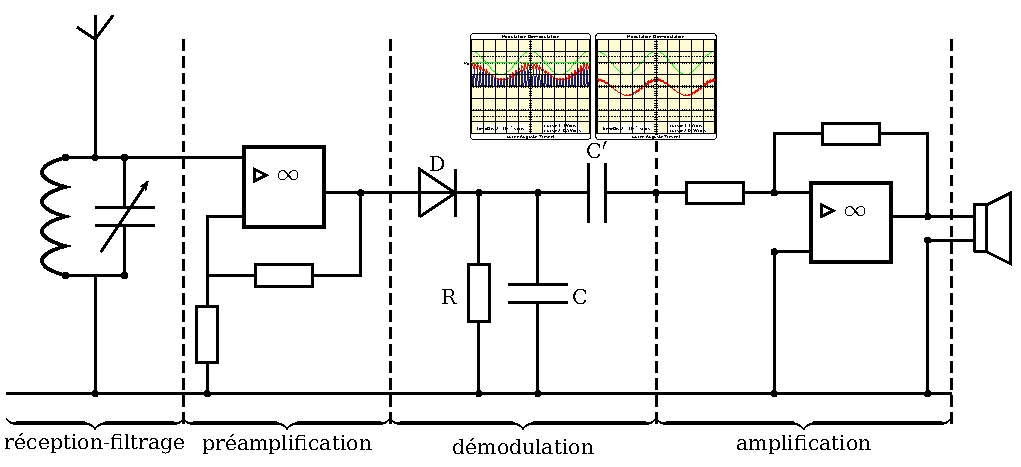
\includegraphics[width=5in]{pst-am-doc.pdf}
\caption{电路图}
\end{figure}

正文内容
\begin{figure}[htp]
\centering
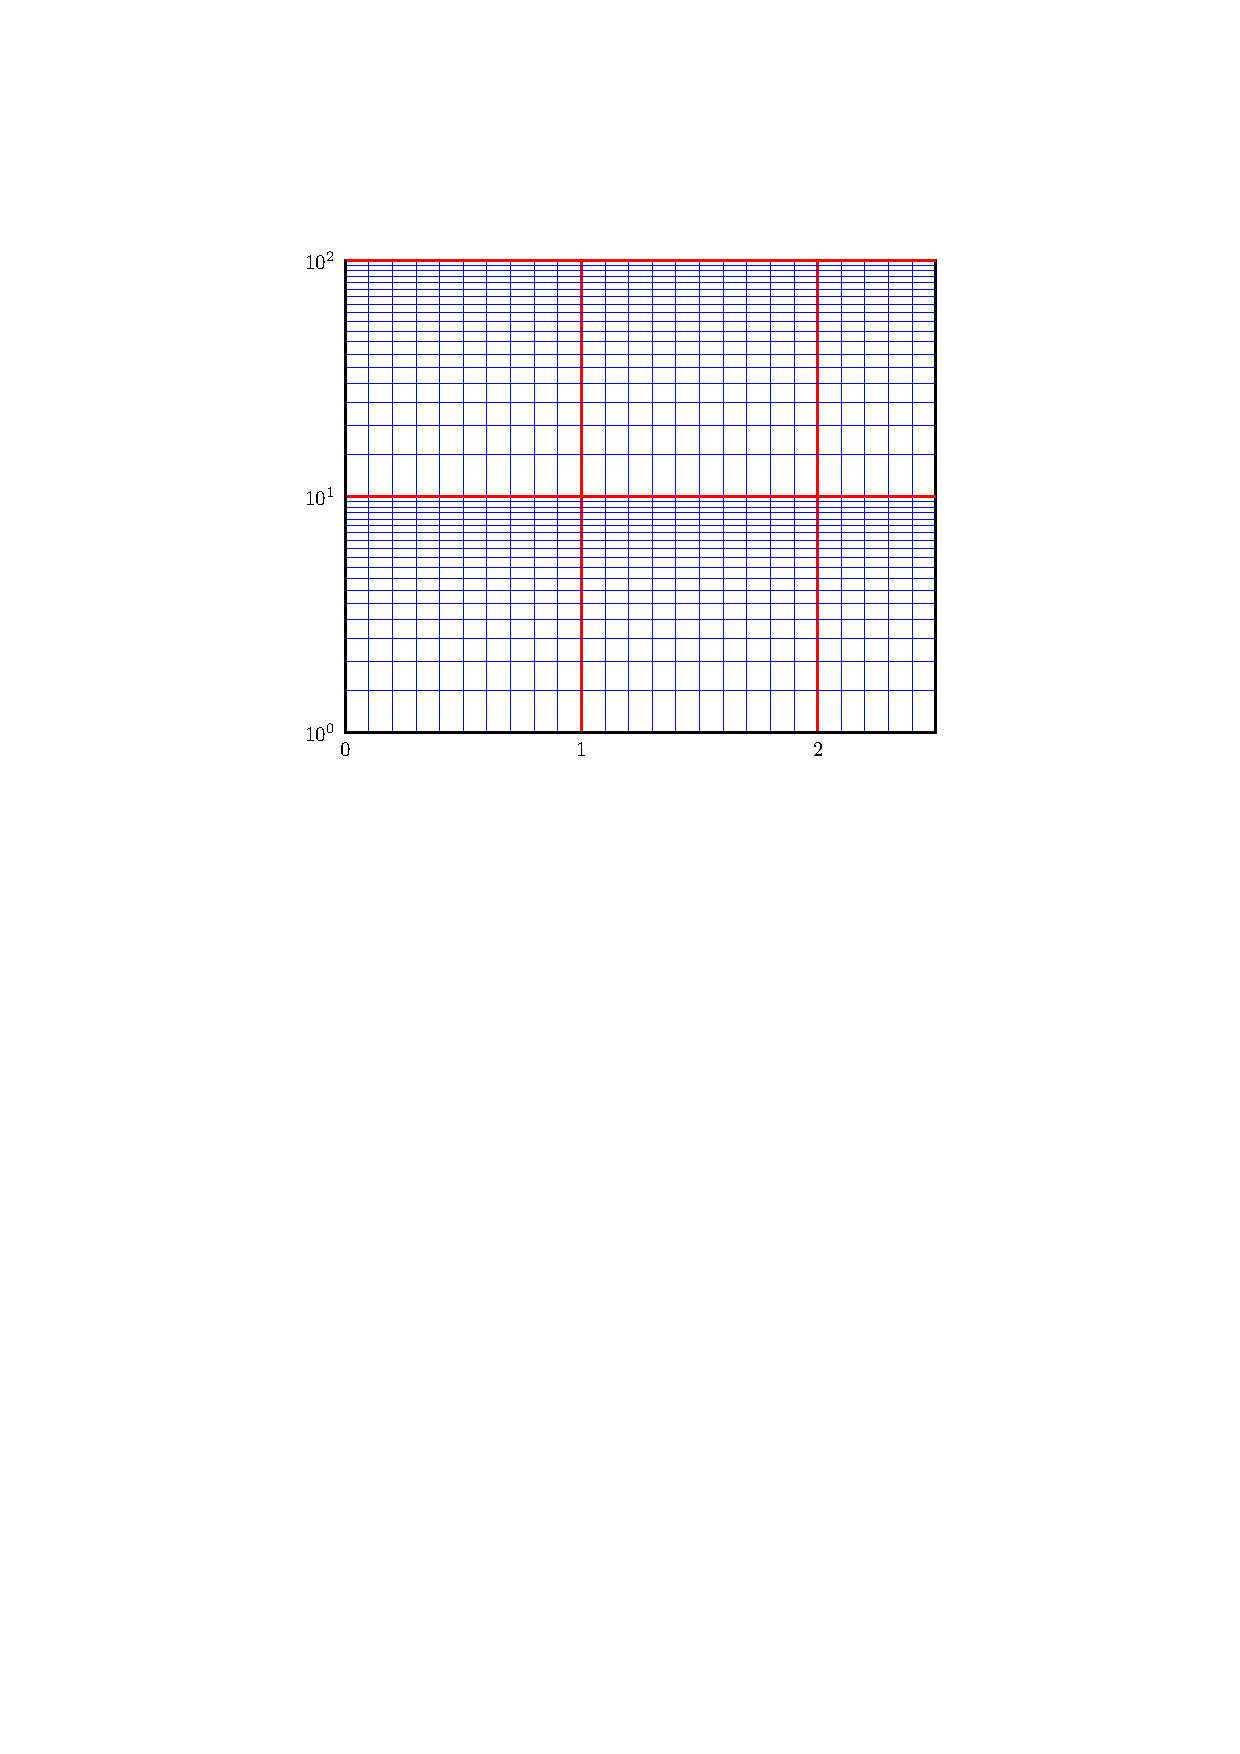
\includegraphics[width=4in]{pst-loglines.pdf}
\caption{对数坐标,在物理实验时可以用到}
\end{figure}

\begin{figure}[htp]
\centering
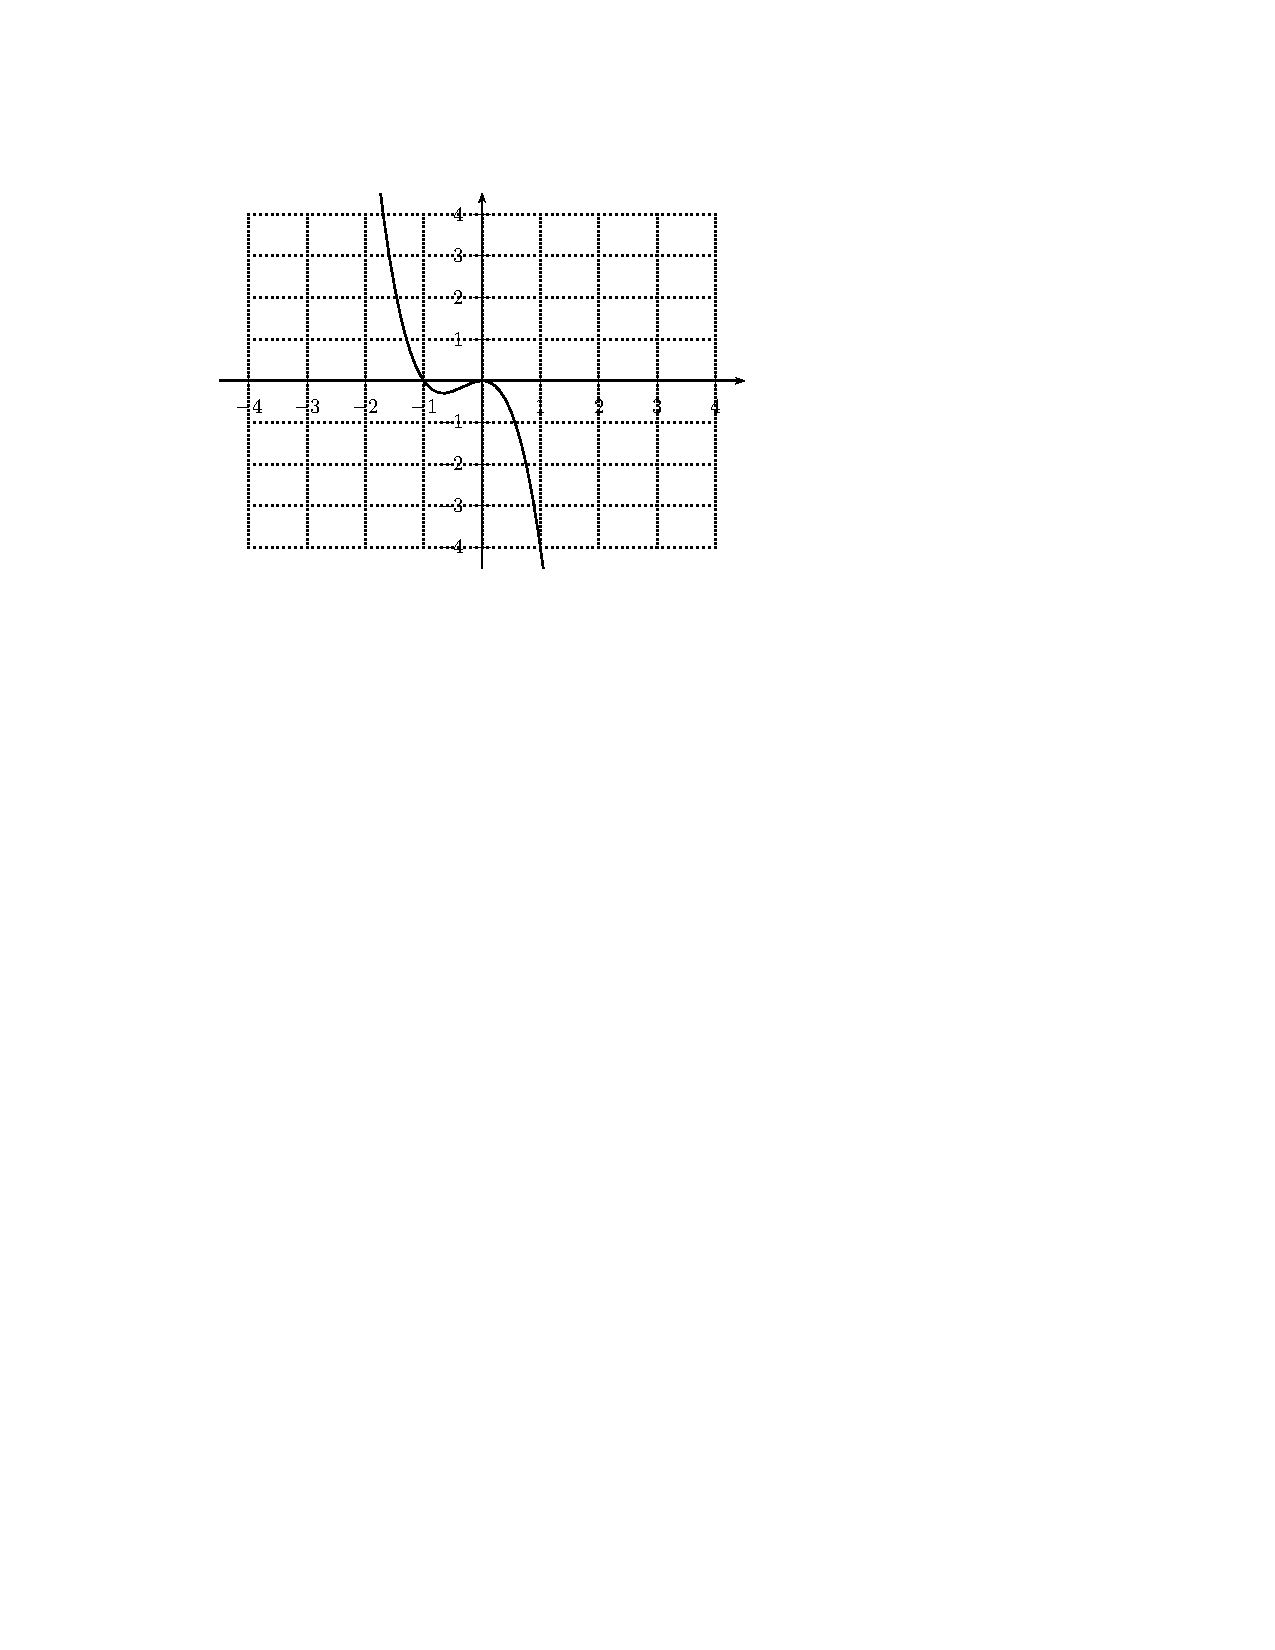
\includegraphics[width=4in]{graph.pdf}
\caption{二维坐标}
\end{figure}
\begin{figure}[htp]
\centering
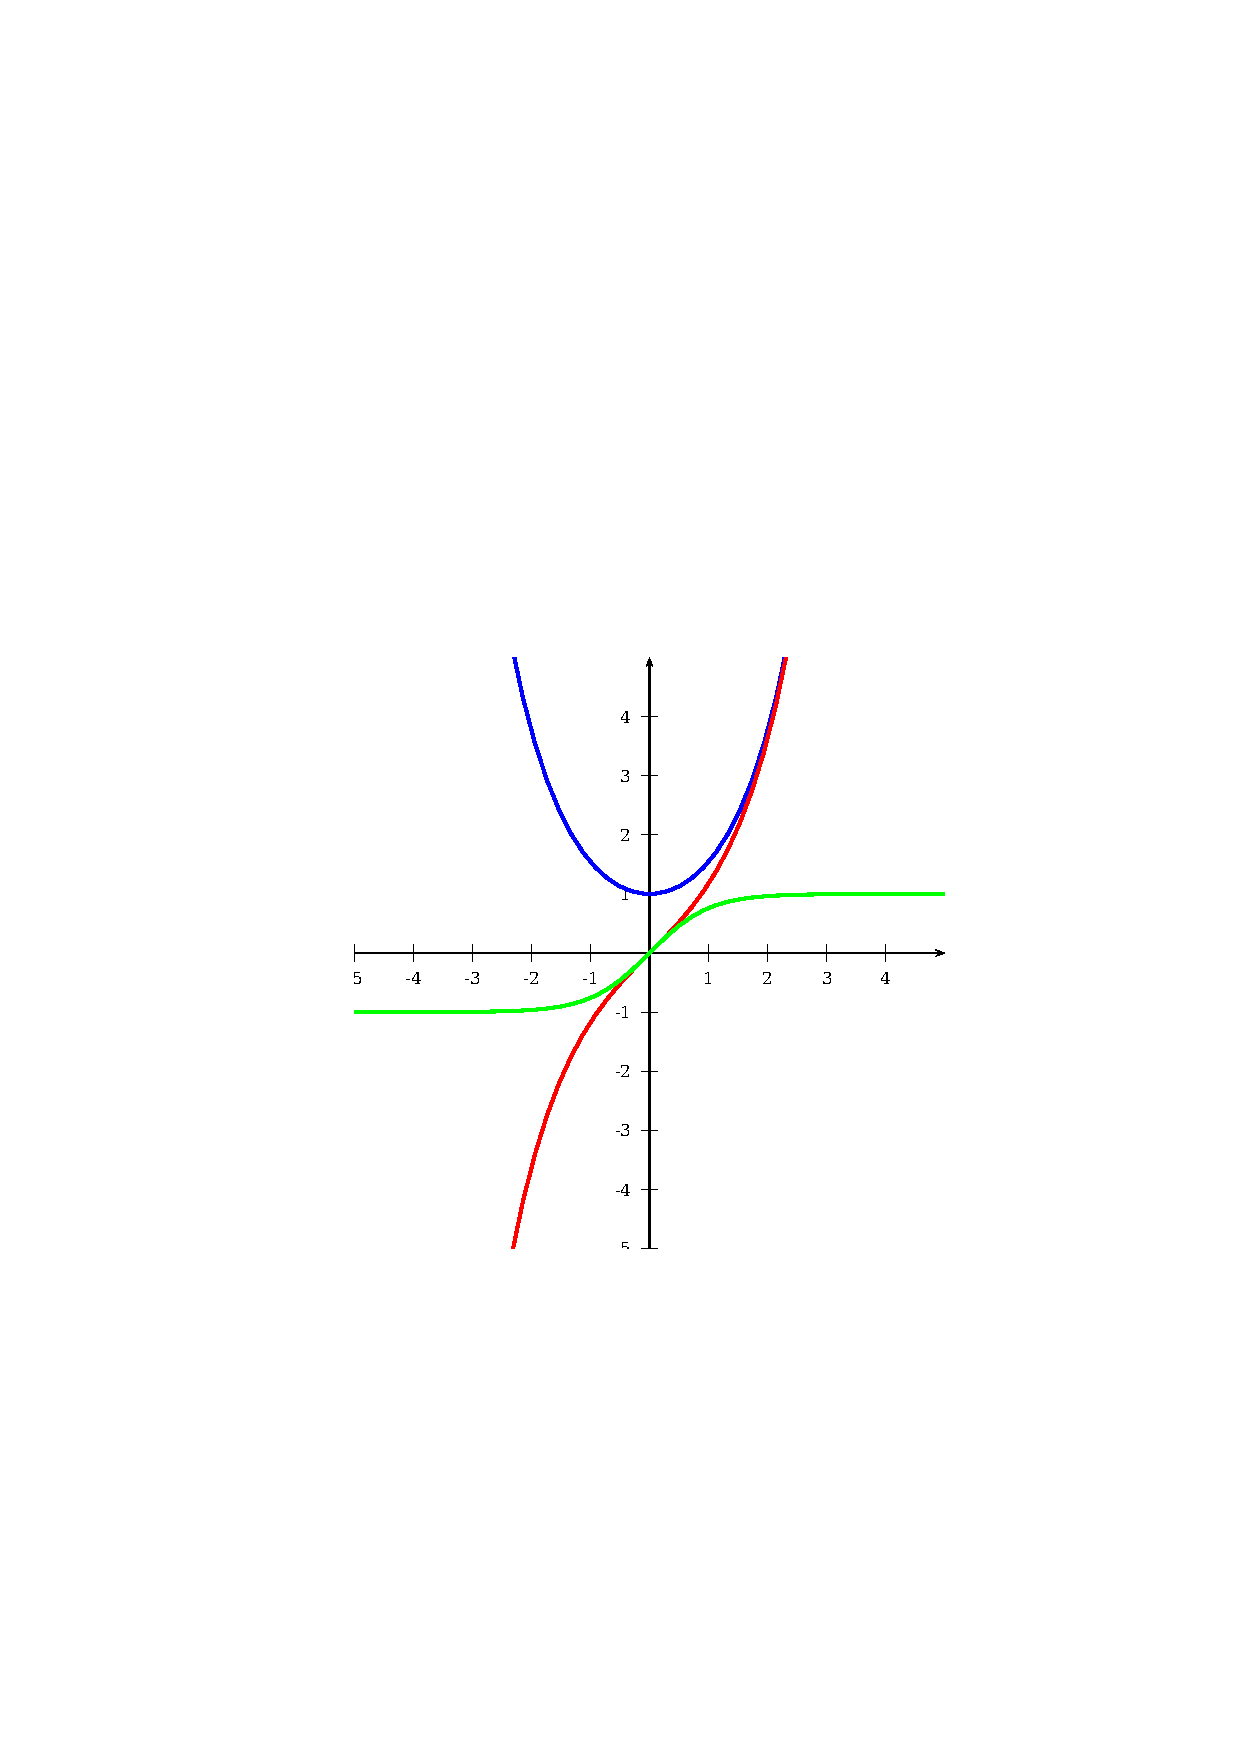
\includegraphics[width=4in]{pst-math-doc.pdf}
\caption{多个函数}
\end{figure}
\subsection{有意思的绘图宏包}
正文内容

\begin{figure}[htp]
\centering
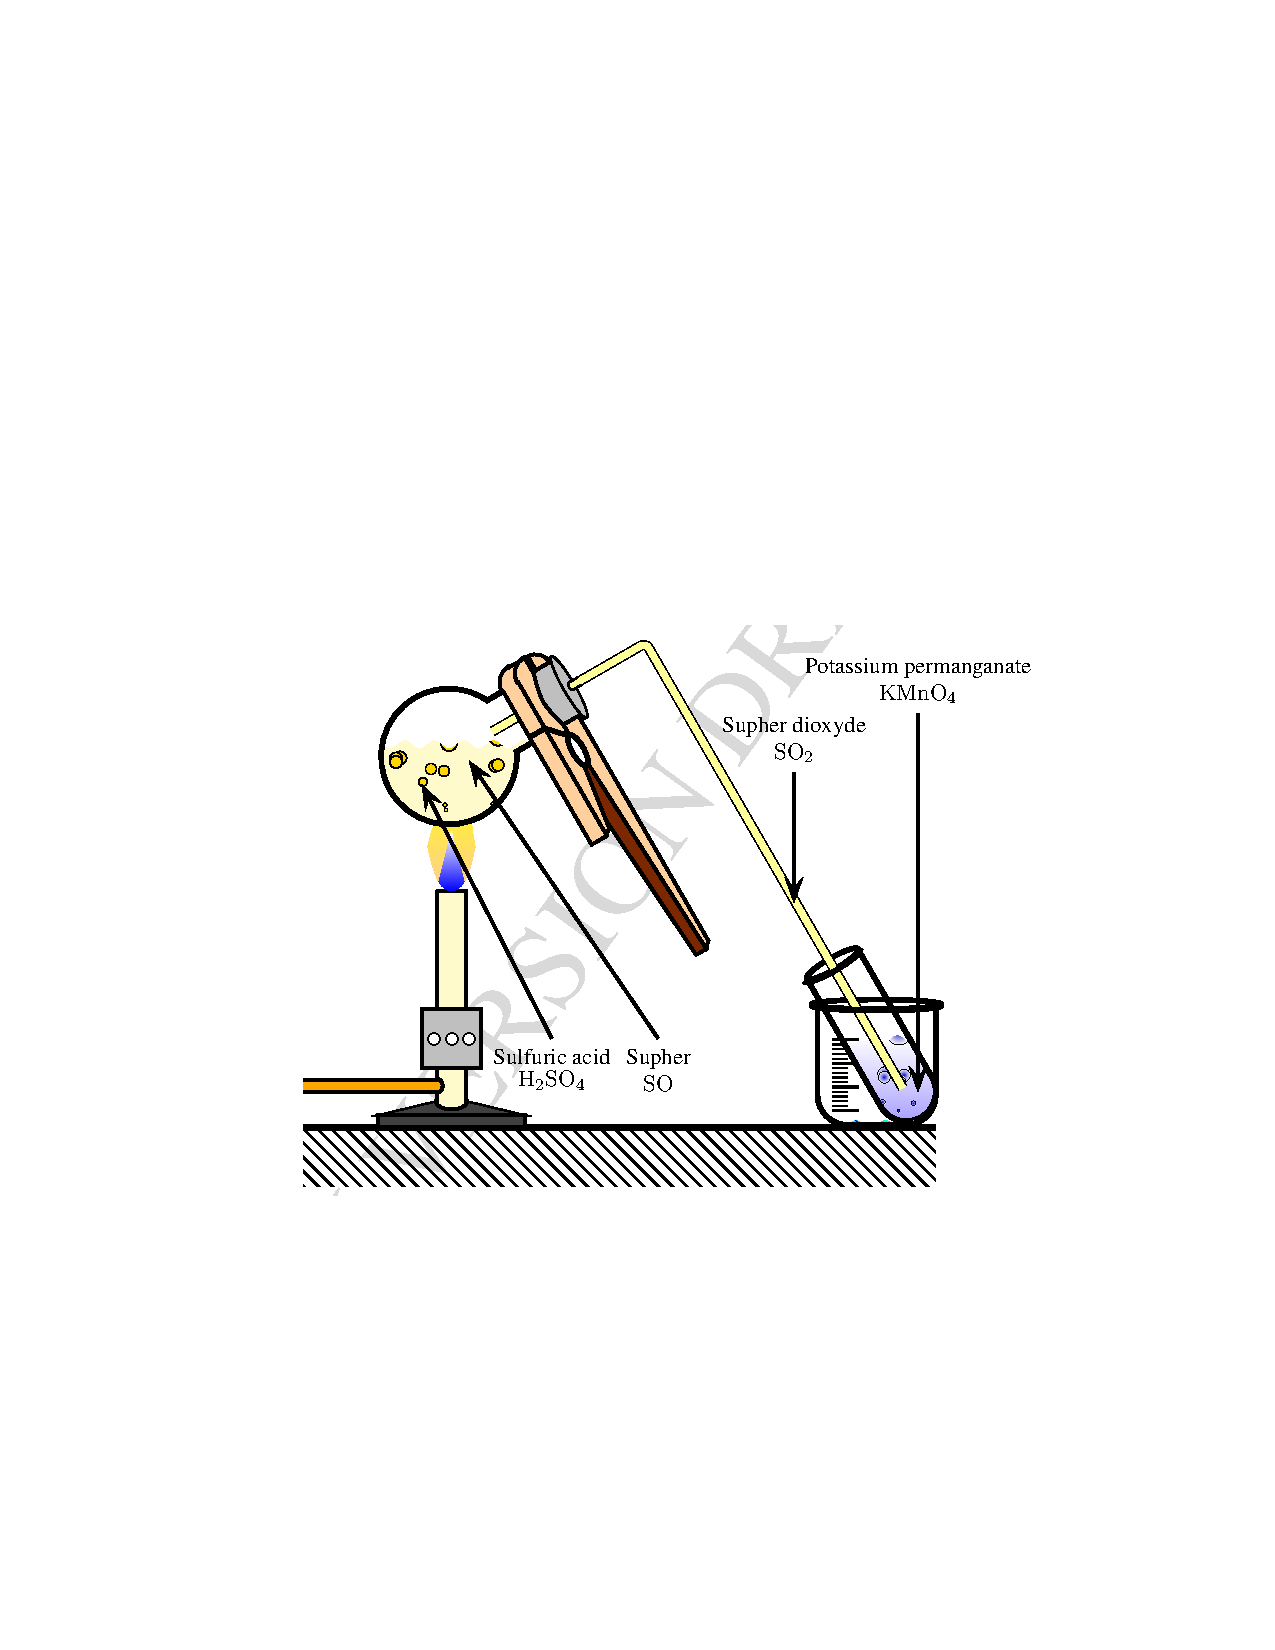
\includegraphics[width=3in]{pstricks-chemical.pdf}
\caption{pstricks宏包绘制的化学实验}
\end{figure}

\subsection{(1.3.2 题目)}
正文内容

正文内容

\begin{table}[H]
\centering
\caption{表 1.2 名称}
\begin{tabular}{|c|c|c|c|c|}
\hline
\makebox[2.07cm][0pt]{} & \makebox[2.07cm][0pt]{} & \makebox[2.07cm][0pt]{} & \makebox[2.07cm][0pt]{} & \makebox[2.07cm][0pt]{} \\
\hline
 & & & & \\
\hline
 & & & & \\
\hline
\end{tabular}
\end{table}
%htbp选项用来指定插图的理想位置,这几个字母分别代表here,top,bottom,float page,也就是就这里、页顶、页尾、浮动页(专门放浮动环境的单独页面)。我们可以使用这几个字母的任意组合,四个字母都写上表示放哪里都无所谓;一般不推荐单独使用h,因为latex自以为它的排版算法是最完美的,不愿意被束缚手脚。
\begin{figure}[htb]
\centering
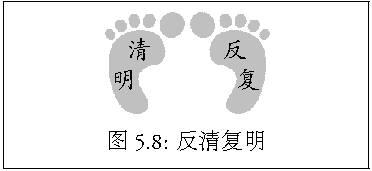
\includegraphics{lnotes2.pdf}
\end{figure}
本模版是根据长安大学毕业论文格式规范制作的\LaTeX{}毕业论文模
板。
本模板是基于国防科技大学的硕博士论文模板,并
按照长安大学毕业论文格式规范开发的\LaTeX{}论文模板,经过完善和修改,目
前已经基本满足了论文规范的要求,而且易用性良好,功能强大。不过,可能还存在着
一些问题,欢迎大家积极使用本模版,反馈遇到的问题,以便不断对其进行改进。
当然这个模板仅仅是一个开始,希望有更多的\TeX{er}能够参与进来,不断改进准确性、
易用性和较好的可维护性,造福需要的兄弟姐妹们。总体上来说,当前这个模板还是很
值得推荐使用的。

本模板的目的旨在推广\LaTeX{}这一优秀的排版软件在长大(尤其是数学相关专业)
的应用,为广大同学提供一个方便、美观的论文模板,减少论文撰写格式方面的麻烦。

\bigskip
Q: ``If you were young again, would you start writing \TeX{} again or would you
use Microsoft Word, or another word processor?"

A: ``I hope to die before I have to use Microsoft Word."

\medskip\hfill Harald K\"{o}nig asking Donald Knuth, T\"{u}bingen, 2 Oct 2001.
\begin{figure}[htp]
\centering
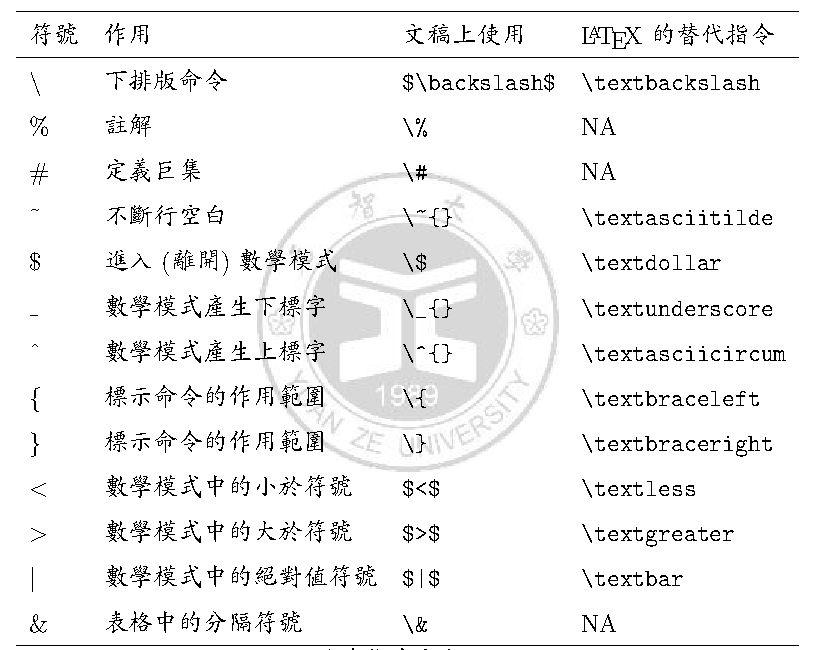
\includegraphics{fuhao.pdf}
\caption{無法直接在\LaTeX{}文稿裏使用的符號字元}
\label{fig:symble}
\end{figure}

图 \ref{fig:symble}的表格列出无法直接在\LaTeX{}文档中使用的符号\footnote{截图自\kai 元智大學光電工程研究所碩士論文}%第一章
% !Mode:: "TeX:UTF-8"
\chapter{论文正文}
\label{chap:main}
本章将进入论文排版的正文, 按元素分主要包括:
{\kai 字体段落,图片表格,公式定理,参考文献}这几部分。
这个样例文件将包括模板中使用到的所有格式、模板中自定义命令到或者特有的东西,
都将被一一介绍,希望大家在排版自己的学位论文前能细致的看一遍,记住样例的格式和
方法,方便上手。

\section{字体段落}
\label{sec:font}
OTF选项下的英文字体我用的是最新的Times New Roman PS Std,如果没有,可以在网上下载,或者安装Adobe的任一款软件,应该会自带字体。实在找不到,你就改成Times New Roman字体吧。等宽英文字体为Courier New。

Adobe中文字体有四种:

{\kai 楷体\verb|\kai|:陈赓,中国湖南湘乡人,军事家。出生将门,其祖父为湘军将领陈翼怀。%
1952年筹办并任人民解放军军事工程学院第一任院长兼政委,培养国防科技人才。1955年被授予大将军衔。}

{\fs 仿宋\verb|\fs|:陈赓,中国湖南湘乡人,军事家。出生将门,其祖父为湘军将领陈翼怀。%
1952年筹办并任人民解放军军事工程学院第一任院长兼政委,培养国防科技人才。1955年被授予大将军衔。}

{\hei 黑体\verb|\hei|:陈赓,中国湖南湘乡人,军事家。出生将门,其祖父为湘军将领陈翼怀。%
1952年筹办并任人民解放军军事工程学院第一任院长兼政委,培养国防科技人才。1955年被授予大将军衔。}

宋体就是正文字体了。下面测试字体大小,\LaTeX{}默认的列表环境会在
条目之间插入过多的行距,在下面这种情况可能正好,若用户需要
{\kai 正文行距}的列表环境,可以使用compactitem环境,记住这点很重要,不要再
用那种自己修改\verb|itemsep|的傻傻的办法了。
\begin{itemize}
\item[初号] {\song\chuhao 陈赓大将}
\item[小初] {\song\xiaochu 陈赓大将}
\item[一号] {\song\yihao 陈赓大将}
\item[小一] {\song\xiaoyi 陈赓大将}
\item[二号] {\song\erhao 陈赓大将}
\item[小二] {\song\xiaoer 陈赓大将}
\item[三号] {\song\sanhao 陈赓大将}
\item[小三] {\song\xiaosan 陈赓大将}
\item[四号] {\song\sihao 陈赓大将}
\item[小四] {\song\xiaosi 陈赓大将}
\item[五号] {\song\wuhao 陈赓大将}
\item[小五] {\song\xiaowu 陈赓大将}
\end{itemize}

\section{表格明细}
\label{sec:figure}
表格是论文的重要组成部分,我们从简单的表格讲起,到复杂的表格为止。
\begin{table}[htbp]
\centering
\begin{tabular}{lllc}
\toprule
操作系统& 发行版& 编辑器& 用户体验\\
\midrule
Windows & MikTeX & TeXnicCenter & \multirow{3}{*}{\centering 爽} \\
Unix/Linux & TeX Live & Emacs \\
Mac OS & MacTeX & TeXShop \\
\bottomrule
\end{tabular}
\end{table}

模板中关于表格的宏包有三个: \textsf{booktabs}、\textsf{array} 和
\textsf{longtabular}。三线表建议使用\textsf{booktabs}中提供的,
包含toprule、midrule 和 bottomrule三条命令,简单干脆!
它们与\textsf{longtable} 能很好的配合使用。下面来看一个表格实例:
\begin{table}[htb]
  \centering
  \begin{minipage}[t]{0.8\linewidth} % 如果想在表格中使用脚注,minipage是个不错的办法
  \caption[模板文件]{模板文件。如果表格的标题很长,那么在表格索引中就会很不美
    观,所以要像 chapter 那样在前面用中括号写一个简短的标题。这个标题会出现在索
    引中。}
  \label{tab:template-files}
    \begin{tabular*}{\linewidth}{lp{10cm}}
      \toprule[1.5pt]
      {\hei 文件名} & {\hei 描述} \\
      \midrule[1pt]
      thesis.tex & 主文档\footnote{表格中的脚注} \\
      chdpaper.cls & 模板类文件。\\
      chdpaper.cfg & 模板配置文。\\
      gbt-7714-2015-numerical.bst   & 参考文献 Bibtex 样式文件。\\
      mychd.sty    & 常用的包和命令写在这里,减轻主文件的负担。\\
      figures文件夹 & 存放图片文件\\
      ref文件夹 & 存放参考文献\\
      data文件夹 & 每章内容\footnote{包括:引言,论文正文,结论以及展望,致谢,附录,附件}\\
      a3cover文件夹 & a3封面,基本上没用\\
      \bottomrule[1.5pt]
    \end{tabular*}
  \end{minipage}
\end{table}

表 \ref{tab:template-files} 列举了本模板主要文件及其功能,基本上来说论文
中最可能用到的就是这种表格形式了。
请大家注意三线表中各条线对应的命令。这个例子还展示了如何在表格中正确使用脚注。
如果你不需要在表格中插入脚注,可以将minipage环境去掉。
由于\LaTeX{}本身不支持在表格中使用\verb|\footnote|,所以我们不得不将表格放在
小页中,而且最好将表格的宽度设置为小页的宽度,这样脚注看起来才更美观。

另外六院的同学在使用模板时需要使用一种固定宽度(往往是页宽,下面的例子由
rongdonghu提供)的表格,内容需要居中且可以自动调整。
解决办法是自定义了一种\verb|tabularx|中的\textbf{Z}环境,在论文模板中,
该命令已添加到\verb|mychd.sty|中。下面是这种情况的实例:

\begin{table}[htbp]
\centering
\begin{minipage}[t]{0.9\linewidth}
\caption{Reed Solomon码的典型应用}
\label{tab:RSuse}
\begin{tabularx}{\linewidth}{cZ}
\toprule[1.5pt]
{\hei 应用领域} & {\hei 编码方案}\\
\midrule[1pt]
磁盘驱动器 & RS(32,28,5)码 \footnote{码长为32、维数为28、最小距离为5} \\
CD & 交叉交织RS码(CIRC) \\
DVD & RS(208,192,17)码、RS(182,172,11)码 \\
光纤通信 & RS(255,229,17)码 \\
\bottomrule[1.5pt]
\end{tabularx}
\end{minipage}
\end{table}

我们经常会在表格下方标注数据来源,或者对表格里面的条目进行解释。前面的脚注是一种
不错的方法,如果你不喜欢minipage方法的脚注。
那么完全可以在表格后面自己写注释,比如表~\ref{tab:tabexamp1}。
\begin{table}[htbp]
  \centering
  \caption{复杂表格示例 1}
  \label{tab:tabexamp1}
  \begin{minipage}[t]{0.8\textwidth}
    \begin{tabularx}{\linewidth}{|l|X|X|X|X|}
      \hline
      \multirow{2}*{\backslashbox{x}{y}}  & \multicolumn{2}{c|}{First Half} & \multicolumn{2}{c|}{Second Half}\\
      \cline{2-5}
      & 1st Qtr &2nd Qtr&3rd Qtr&4th Qtr \\
      \hline
      \multirow{2}*{East$^{*}$} &   20.4&   27.4&   90&     20.4 \\
       &   30.6 &   38.6 &   34.6 &  31.6 \\
      West$^{**}$ &   30.6 &   38.6 &   34.6 &  31.6 \\
      \hline
    \end{tabularx}\\[2pt]
    \footnotesize
    *:东部\\
    **:西部
  \end{minipage}
\end{table}

此外,表~\ref{tab:tabexamp1} 同时还演示了另外三个功能:1)通过 \textsf{tabularx} 的
 \texttt{|X|} 扩展实现表格内容自动调整;2)通过命令 \verb|\backslashbox| 在表头部分
插入反斜线(WORD中很简单,但\LaTeX{}做表格需要一定的(极大的)想象力);3)就是
使用\verb|multirow|和\verb|multicolumn|命令。

不可否认 \LaTeX{} 的表格功能没有想象中的那么强大,不过只要你足够认真,足够细致,那么
同样可以排出来非常复杂非常漂亮的表格。可是科技论文中那么复杂表格有什么用呢?
上面那个表格就够用啦。

浮动体的并排放置一般有两种情况:1)二者没有关系,为两个独立的浮动体;2)二者隶属
于同一个浮动体。对表格来说并排表格既可以像表~\ref{tab:parallel1}、表~\ref{tab:parallel2}
使用小页环境,也可以如表~\ref{tab:subtable}使用子表格来做。
图与表同出一源,后面我们将讲解子图(subfloat)的例子。
\begin{table}[htb]
\centering
\noindent\begin{minipage}{0.45\textwidth}
\centering
\caption{第一个并排子表格}
\label{tab:parallel1}
\begin{tabular}{p{2cm}p{2cm}}
\toprule[1.5pt]
111 & 222 \\\midrule[1pt]
222 & 333 \\\bottomrule[1.5pt]
\end{tabular}
\end{minipage}
\begin{minipage}{0.45\textwidth}
\centering
\caption{第二个并排子表格}
\label{tab:parallel2}
\begin{tabular}{p{2cm}p{2cm}}
\toprule[1.5pt]
111 & 222 \\\midrule[1pt]
222 & 333 \\\bottomrule[1.5pt]
\end{tabular}
\end{minipage}
\end{table}
\begin{table}[htbp]
\centering
\caption{并排子表格}
\label{tab:subtable}
\subfloat[第一个子表格]{
\begin{tabular}{p{2cm}p{2cm}}
\toprule[1.5pt]
111 & 222 \\\midrule[1pt]
222 & 333 \\\bottomrule[1.5pt]
\end{tabular}}\hskip2cm
\subfloat[第二个子表格]{
\begin{tabular}{p{2cm}p{2cm}}
\toprule[1.5pt]
111 & 222 \\\midrule[1pt]
222 & 333 \\\bottomrule[1.5pt]
\end{tabular}}
\end{table}

如果您要排版的表格长度超过一页,那么推荐使用\textsf{longtable}命令。
这里随便敲入一些无关的文字,使得正文看上去不是那么的少。
表~\ref{tab:performance} 就是 \textsf{longtable} 的简单示例。
\begin{longtable}{ll}
\multicolumn{2}{r}{接上页} \\
\toprule
作者& 作品\\
\midrule
\endhead
\caption{长表格} \\
\toprule
作者& 作品\\
\midrule
\endfirsthead
\bottomrule
\multicolumn{2}{r}{接下页\dots} \\
\endfoot
\bottomrule
\endlastfoot
白居易& 汉皇重色思倾国,御宇多年求不得。\\
 & 杨家有女初长成,养在深闺人未识。\\
& 天生丽质难自弃,一朝选在君王侧。\\
 & 回眸一笑百媚生,六宫粉黛无颜色。\\
& 春寒赐浴华清池,温泉水滑洗凝脂。\\
 & 侍儿扶起娇无力,始是新承恩泽时。\\
& 云鬓花颜金步摇,芙蓉帐暖度春宵。\\
 & 春宵苦短日高起,从此君王不早朝。\\
& 承欢侍宴无闲暇,春从春游夜专夜。\\
 & 后宫佳丽三千人,三千宠爱在一身。\\
& 金屋妆成娇侍夜,玉楼宴罢醉和春。\\
 & 姊妹弟兄皆列土,可怜光彩生门户。\\
& 遂令天下父母心,不重生男重生女。\\
 & 骊宫高处入青云,仙乐风飘处处闻。\\
& 缓歌慢舞凝丝竹,尽日君王看不足。\\
 & 渔阳鼙鼓动地来,惊破霓裳羽衣曲。\\
& 九重城阙烟尘生,千乘万骑西南行。\\
 & 翠华摇摇行复止,西出都门百余里。\\
& 六军不发无奈何,宛转蛾眉马前死。\\
 & 花钿委地无人收,翠翅金雀玉搔头。\\
& 君王掩面救不得,回看血泪相和流。\\
 & 黄埃散漫风萧索,云栈萦纡登剑阁。\\
& 峨嵋山下少人行,旌旗无光日色薄。\\
 & 蜀江水碧蜀山青,圣主朝朝暮暮情。\\
& 行宫见月伤心色,夜雨闻铃断肠声。\\
 \end{longtable}
\begin{longtable}[c]{c*{6}{r}}
\caption{实验数据}\label{tab:performance}\\
\toprule[1.5pt]
 测试程序 & \multicolumn{1}{c}{正常运行} & \multicolumn{1}{c}{同步}
& \multicolumn{1}{c}{检查点}   & \multicolumn{1}{c}{卷回恢复}
& \multicolumn{1}{c}{进程迁移} & \multicolumn{1}{c}{检查点} 	\\
& \multicolumn{1}{c}{时间 (s)} & \multicolumn{1}{c}{时间 (s)}
& \multicolumn{1}{c}{时间 (s)} & \multicolumn{1}{c}{时间 (s)}
& \multicolumn{1}{c}{时间 (s)} &  文件(KB)			\\
\midrule[1pt]%
\endfirsthead%

\multicolumn{7}{c}{\heiti\sffamily 续表~\thetable\hskip1em 实验数据}\\

\toprule[1.5pt]
 测试程序 & \multicolumn{1}{c}{正常运行} & \multicolumn{1}{c}{同步}
& \multicolumn{1}{c}{检查点}   & \multicolumn{1}{c}{卷回恢复}
& \multicolumn{1}{c}{进程迁移} & \multicolumn{1}{c}{检查点} 	\\
& \multicolumn{1}{c}{时间 (s)} & \multicolumn{1}{c}{时间 (s)}
& \multicolumn{1}{c}{时间 (s)} & \multicolumn{1}{c}{时间 (s)}
& \multicolumn{1}{c}{时间 (s)} &  文件(KB)			\\
\midrule[1pt]%
\endhead%
\hline%

\multicolumn{7}{r}{续下页}%

\endfoot%
\endlastfoot%
CG.A.2 & 23.05   & 0.002 & 0.116 & 0.035 & 0.589 & 32491  \\
CG.A.4 & 15.06   & 0.003 & 0.067 & 0.021 & 0.351 & 18211  \\
CG.A.8 & 13.38   & 0.004 & 0.072 & 0.023 & 0.210 & 9890   \\
CG.B.2 & 867.45  & 0.002 & 0.864 & 0.232 & 3.256 & 228562 \\
CG.B.4 & 501.61  & 0.003 & 0.438 & 0.136 & 2.075 & 123862 \\
CG.B.8 & 384.65  & 0.004 & 0.457 & 0.108 & 1.235 & 63777  \\
MG.A.2 & 112.27  & 0.002 & 0.846 & 0.237 & 3.930 & 236473 \\
MG.A.4 & 59.84   & 0.003 & 0.442 & 0.128 & 2.070 & 123875 \\
MG.A.8 & 31.38   & 0.003 & 0.476 & 0.114 & 1.041 & 60627  \\
MG.B.2 & 526.28  & 0.002 & 0.821 & 0.238 & 4.176 & 236635 \\
MG.B.4 & 280.11  & 0.003 & 0.432 & 0.130 & 1.706 & 123793 \\
MG.B.8 & 148.29  & 0.003 & 0.442 & 0.116 & 0.893 & 60600  \\
LU.A.2 & 2116.54 & 0.002 & 0.110 & 0.030 & 0.532 & 28754  \\
LU.A.4 & 1102.50 & 0.002 & 0.069 & 0.017 & 0.255 & 14915  \\
LU.A.8 & 574.47  & 0.003 & 0.067 & 0.016 & 0.192 & 8655   \\
LU.B.2 & 9712.87 & 0.002 & 0.357 & 0.104 & 1.734 & 101975 \\
LU.B.4 & 4757.80 & 0.003 & 0.190 & 0.056 & 0.808 & 53522  \\
LU.B.8 & 2444.05 & 0.004 & 0.222 & 0.057 & 0.548 & 30134  \\
EP.A.2 & 123.81  & 0.002 & 0.010 & 0.003 & 0.074 & 1834   \\
EP.A.4 & 61.92   & 0.003 & 0.011 & 0.004 & 0.073 & 1743   \\
EP.A.8 & 31.06   & 0.004 & 0.017 & 0.005 & 0.073 & 1661   \\
EP.B.2 & 495.49  & 0.001 & 0.009 & 0.003 & 0.196 & 2011   \\
EP.B.4 & 247.69  & 0.002 & 0.012 & 0.004 & 0.122 & 1663   \\
EP.B.8 & 126.74  & 0.003 & 0.017 & 0.005 & 0.083 & 1656   \\
\bottomrule[1.5pt]
\end{longtable}
\subsection{宽表格\upcite{baotailei}}
如表格 \ref{tab:tabexampz}太宽时可以使用Fairbairns等人的rotating宏包。其方法很简
单,用sidewaystable环境替代table环境即可。
\begin{sidewaystable}[htbp]
  \centering
  \caption{宽表格示例}
  \label{tab:tabexampz}
  \begin{minipage}[t]{0.8\textwidth}
    \begin{tabularx}{\linewidth}{|l|X|X|X|X|}
      \hline
      \multirow{2}*{\backslashbox{x}{y}}  & \multicolumn{2}{c|}{First Half} & \multicolumn{2}{c|}{Second Half}\\
      \cline{2-5}
      & 1st Qtr &2nd Qtr&3rd Qtr&4th Qtr \\
      \hline
      \multirow{2}*{East$^{*}$} &   20.4&   27.4&   90&     20.4 \\
       &   30.6 &   38.6 &   34.6 &  31.6 \\
      West$^{**}$ &   30.6 &   38.6 &   34.6 &  31.6 \\
      \multirow{2}*{North$^{*}$} &   20.4&   27.4&   90&     20.4 \\
       &   30.6 &   38.6 &   34.6 &  31.6 \\
      South$^{**}$ &   30.6 &   38.6 &   34.6 &  31.6 \\
      \hline
    \end{tabularx}\\[2pt]
    \footnotesize
    *:东部\\
    **:西部
  \end{minipage}
\end{sidewaystable}

\section{绘图插图}
\mingyan{有图有真相}{莎士比亚}

本模板不再预先装载任何绘图包(如 \textsf{pstricks,pgf} 等),完全由你自己来决定。
个人觉得 \textsf{pgf} 不错,不依赖于 Postscript。此外还有很多针对 \LaTeX{} 的
 GUI 作图工具,如 XFig(jFig), WinFig, Tpx, Ipe, Dia, Inkscape, LaTeXPiX,
jPicEdt 等等。本人强烈推荐\textsf{Ipe}。

一般图形都是处在浮动环境中。之所以称为浮动是指最终排版效果图形的位置不一定与源文
件中的位置对应,这也是刚使用 \LaTeX{} 同学可能遇到的问题。
如果要强制固定浮动图形的位置,请使用 \textsf{float} 宏包,
它提供了 \texttt{[H]}(意思是图片就给我放在这里\textcolor{red}{H}ere)参数,
但是除非特别需要,不建议使用\texttt{[H]},而是推荐使用\texttt{[htbp]},
给\LaTeX{}更多选择。比如图~\ref{fig:ipe}。
\begin{figure}[htbp] % use float package if you want it here
  \centering
  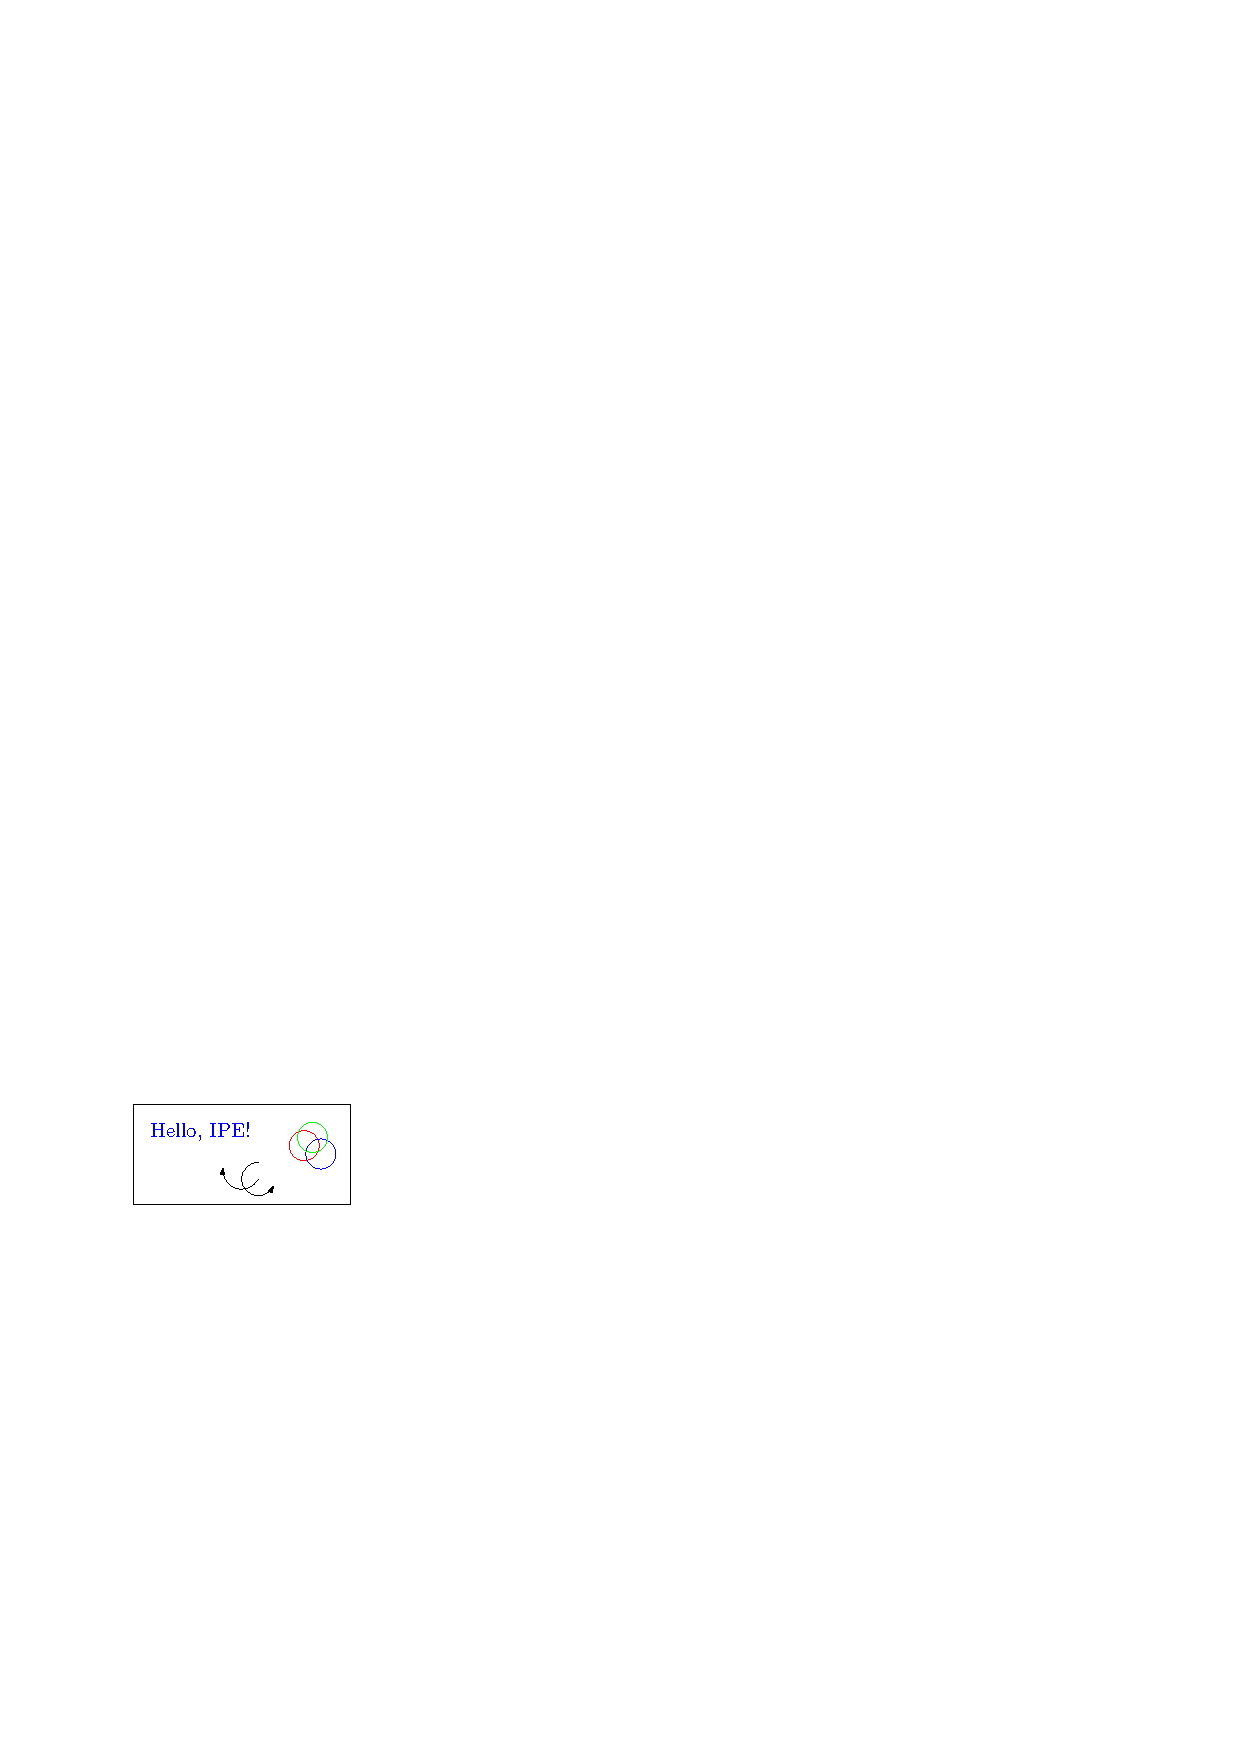
\includegraphics[width=3in]{hello}
  \caption{利用IPE制图}
  \label{fig:ipe}
\end{figure}

若子图共用一个计数器,
那么请看图~\ref{fig:big1},它包含两个小图,分别是图~\ref{fig:subfig1}
和图~\ref{fig:subfig2}。这里推荐使用\verb|\subfloat|,{\bf 不要再用}
\verb|\subfigure|和\verb|\subtable|。
\begin{figure}[htb]
  \centering%
  \subfloat[第一个小图形]{%
    \label{fig:subfig1}
    
\includegraphics[height=2cm]{chdblacklogo.pdf}}\hspace{4em}%
  \subfloat[第二个小图形。如果标题很长的话,它会自动换行,这个 caption 就是这样的例子]{%
    \label{fig:subfig2}
    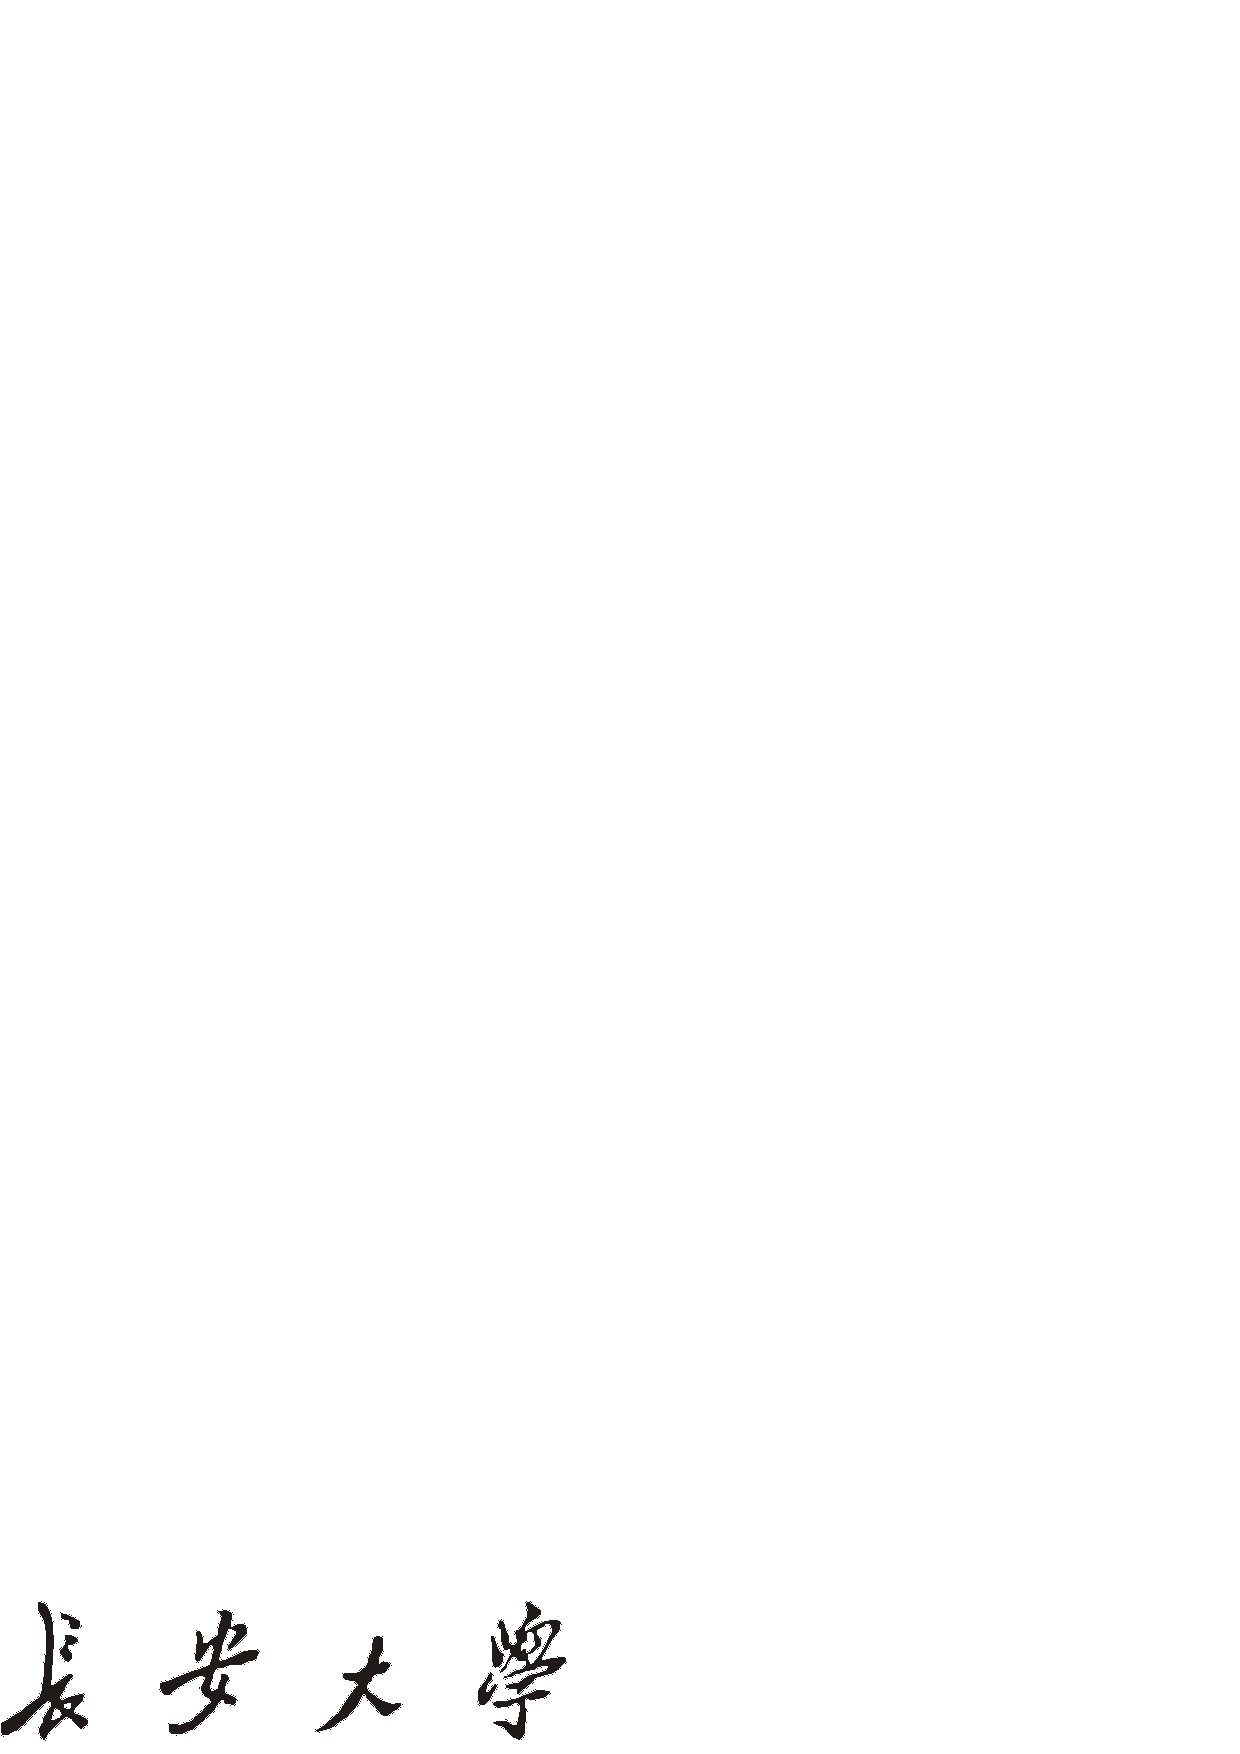
\includegraphics[height=2cm]{chdname.pdf}}
  \caption{包含子图形的大图形}
  \label{fig:big1}
\end{figure}

而下面这个例子显示并排$3\times2$的图片,见图\ref{fig:subfig:3x2}:
\begin{figure}[htb]
\centering
\subfloat[]{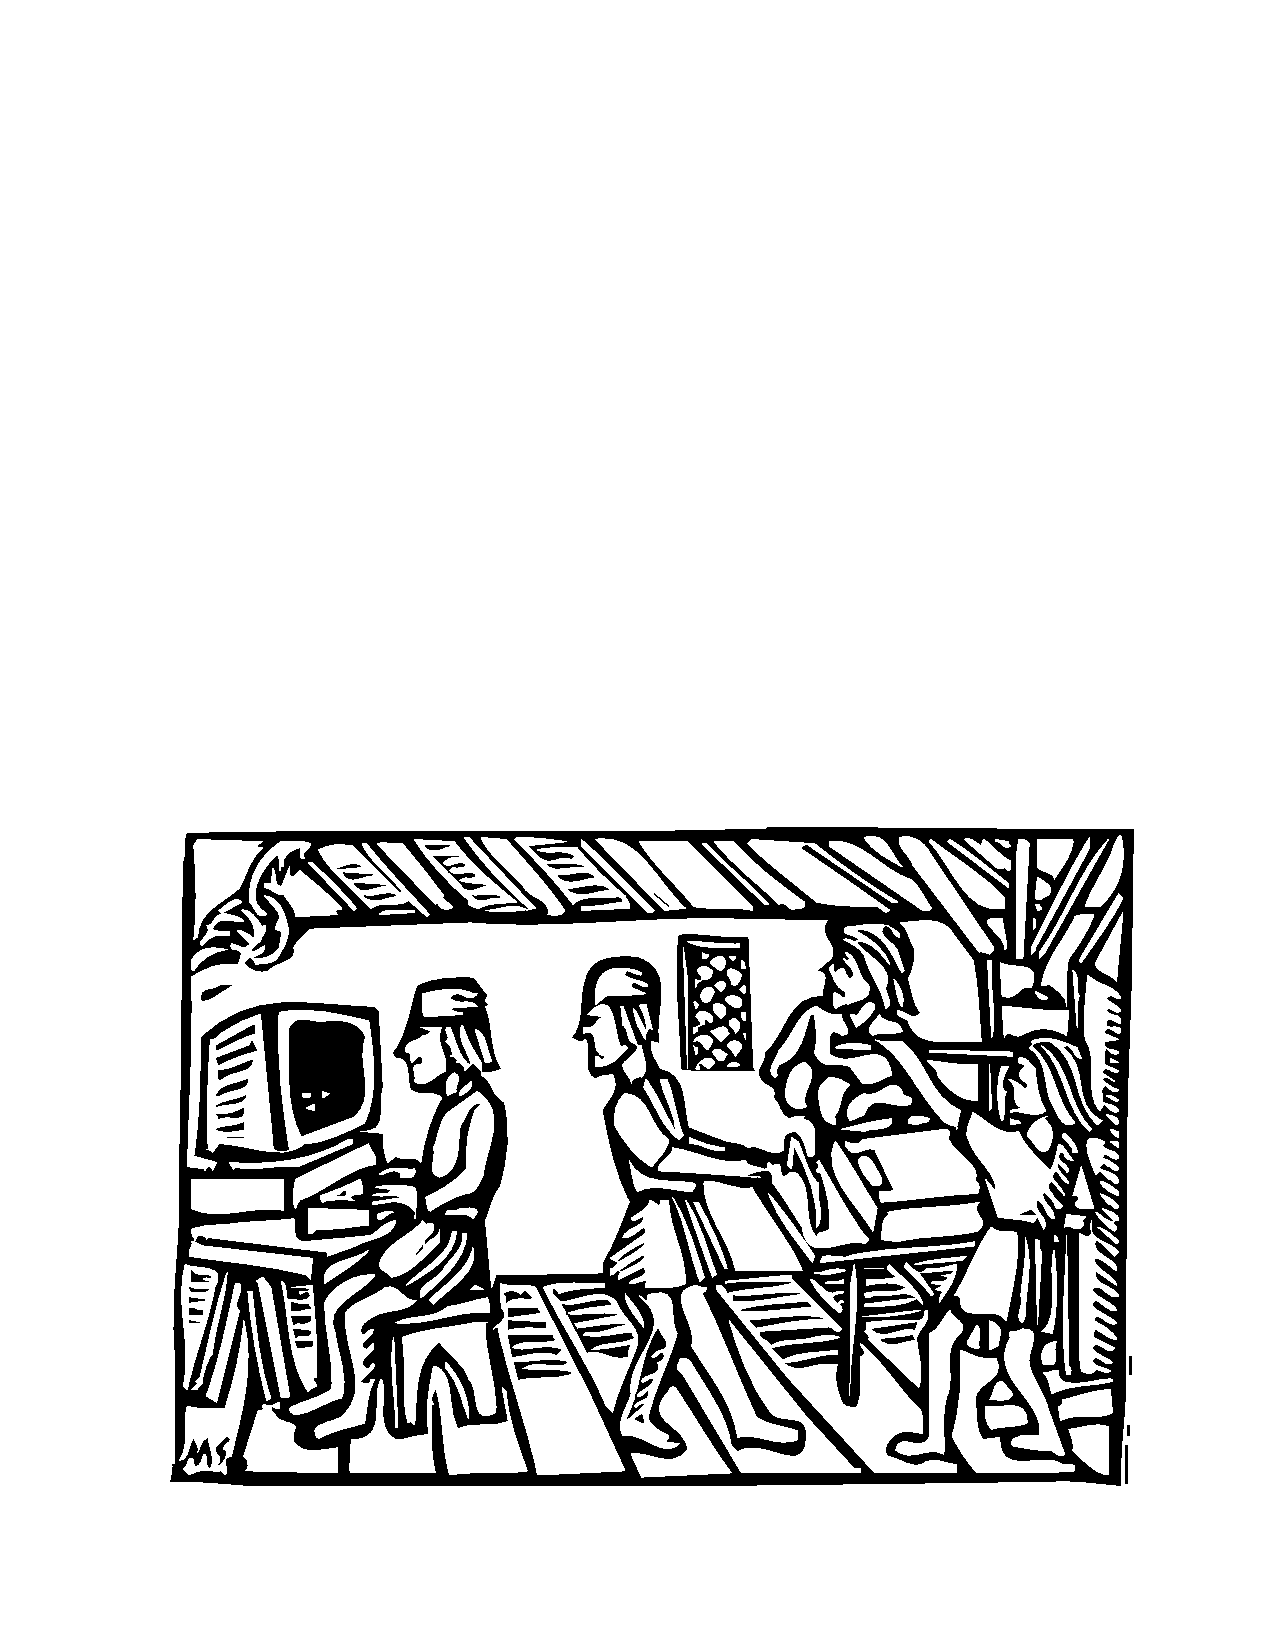
\includegraphics[width=.27\textwidth]{typography}} \qquad
\subfloat[]{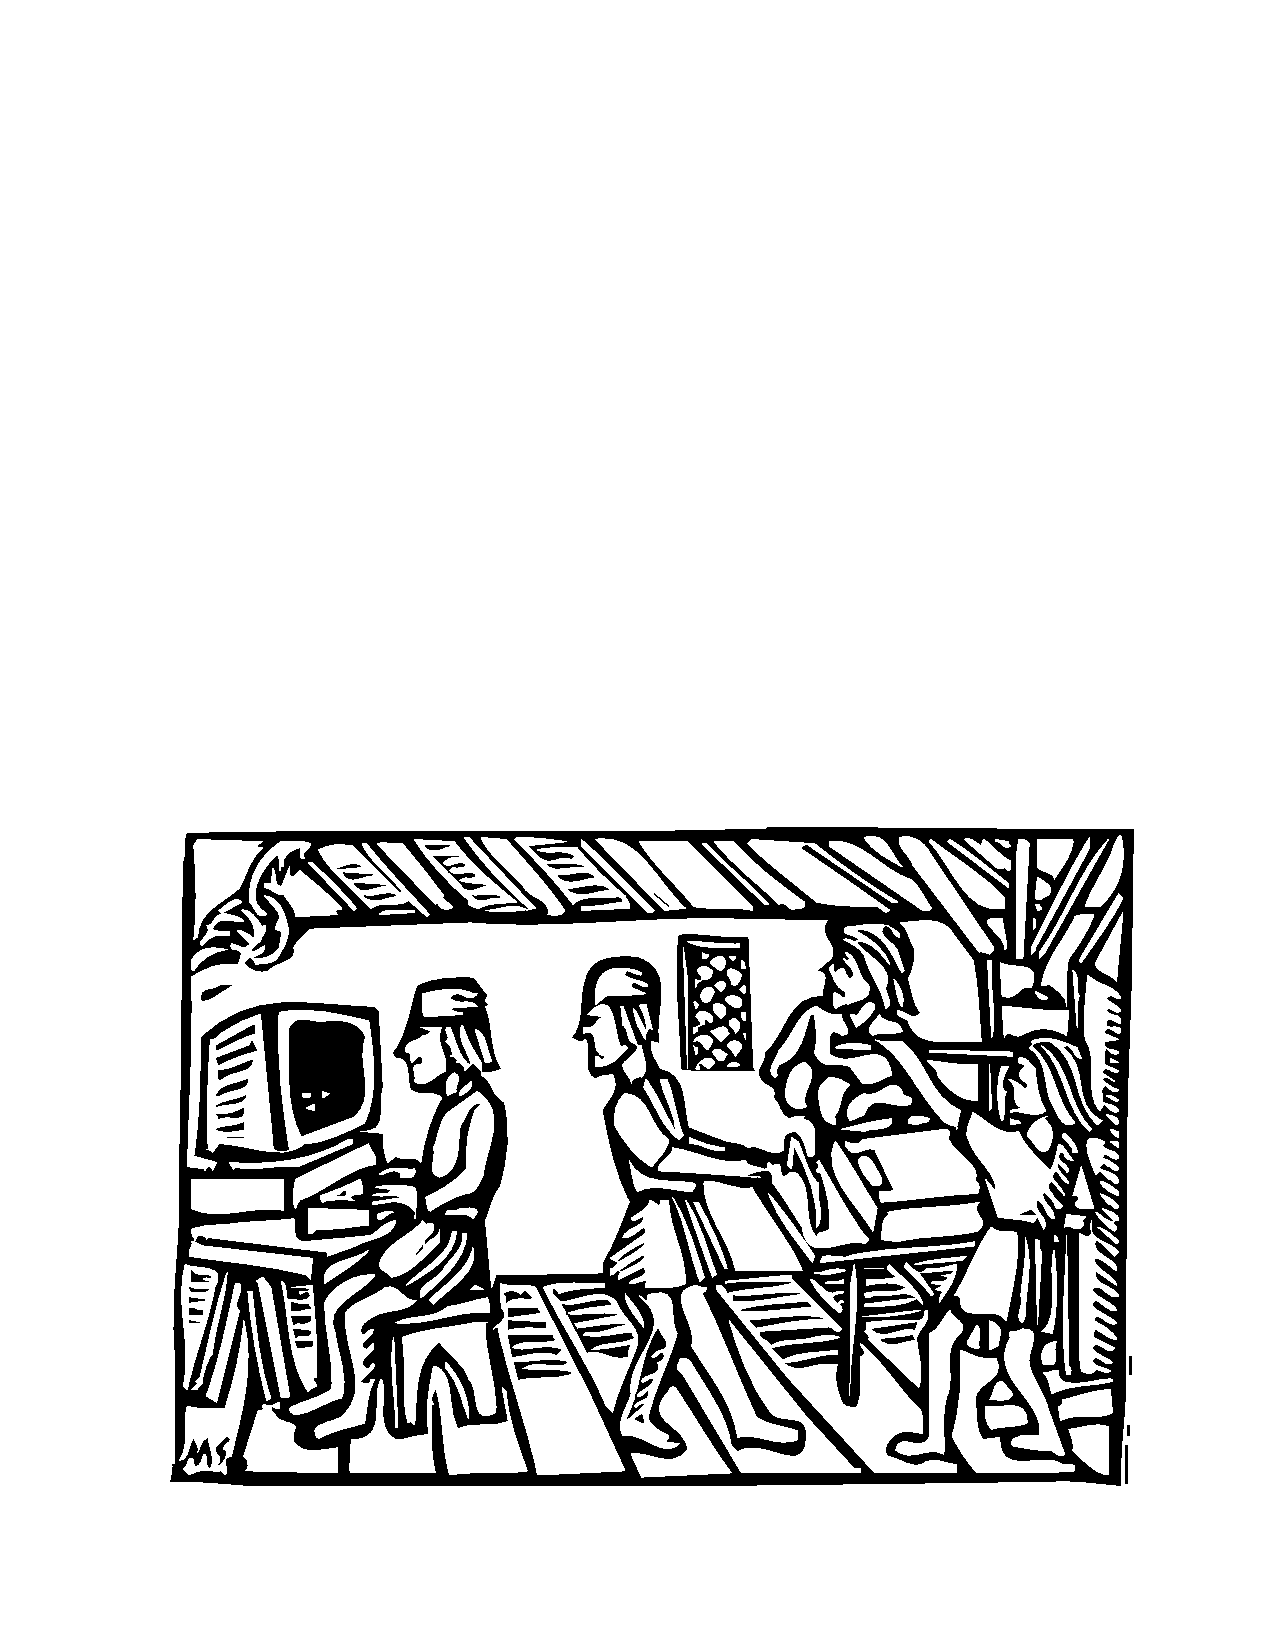
\includegraphics[width=.27\textwidth]{typography}} \qquad
\subfloat[]{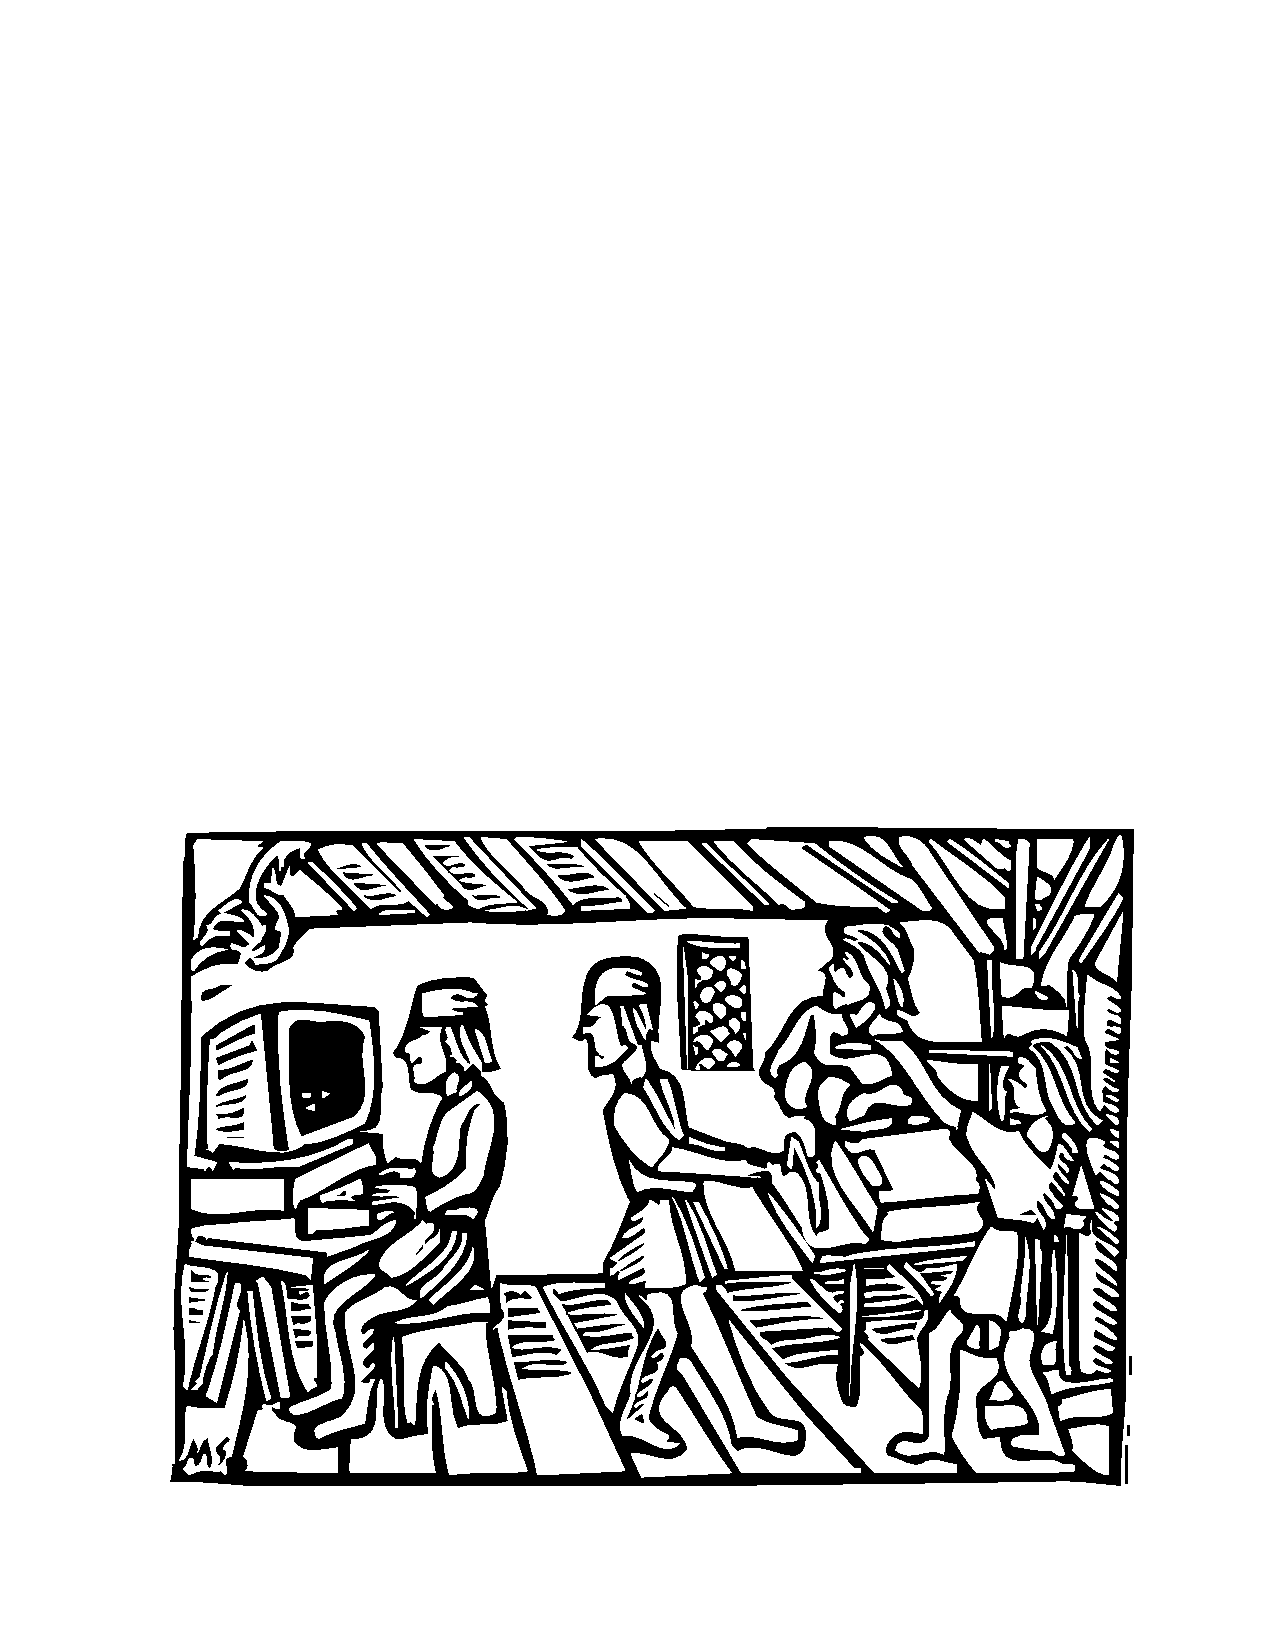
\includegraphics[width=.27\textwidth]{typography}} \qquad
\subfloat[]{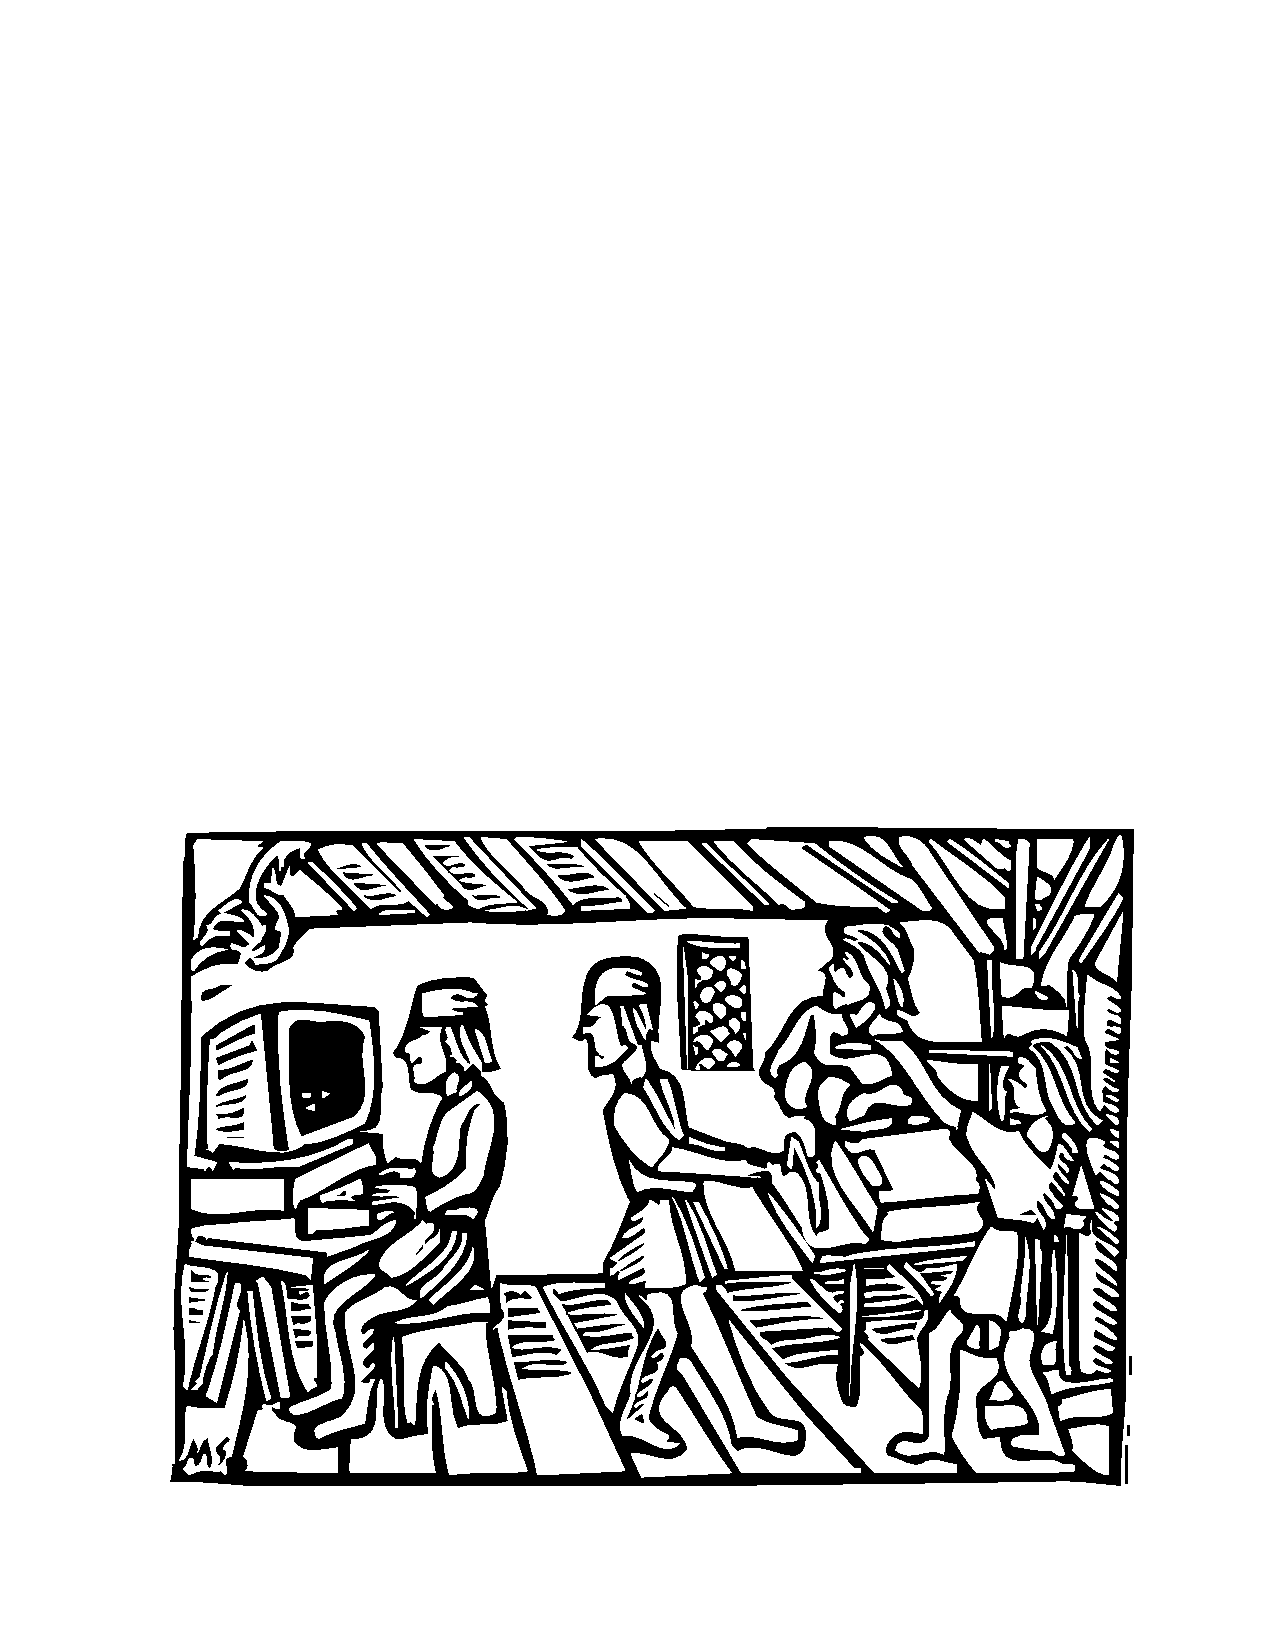
\includegraphics[width=.27\textwidth]{typography}} \qquad
\subfloat[]{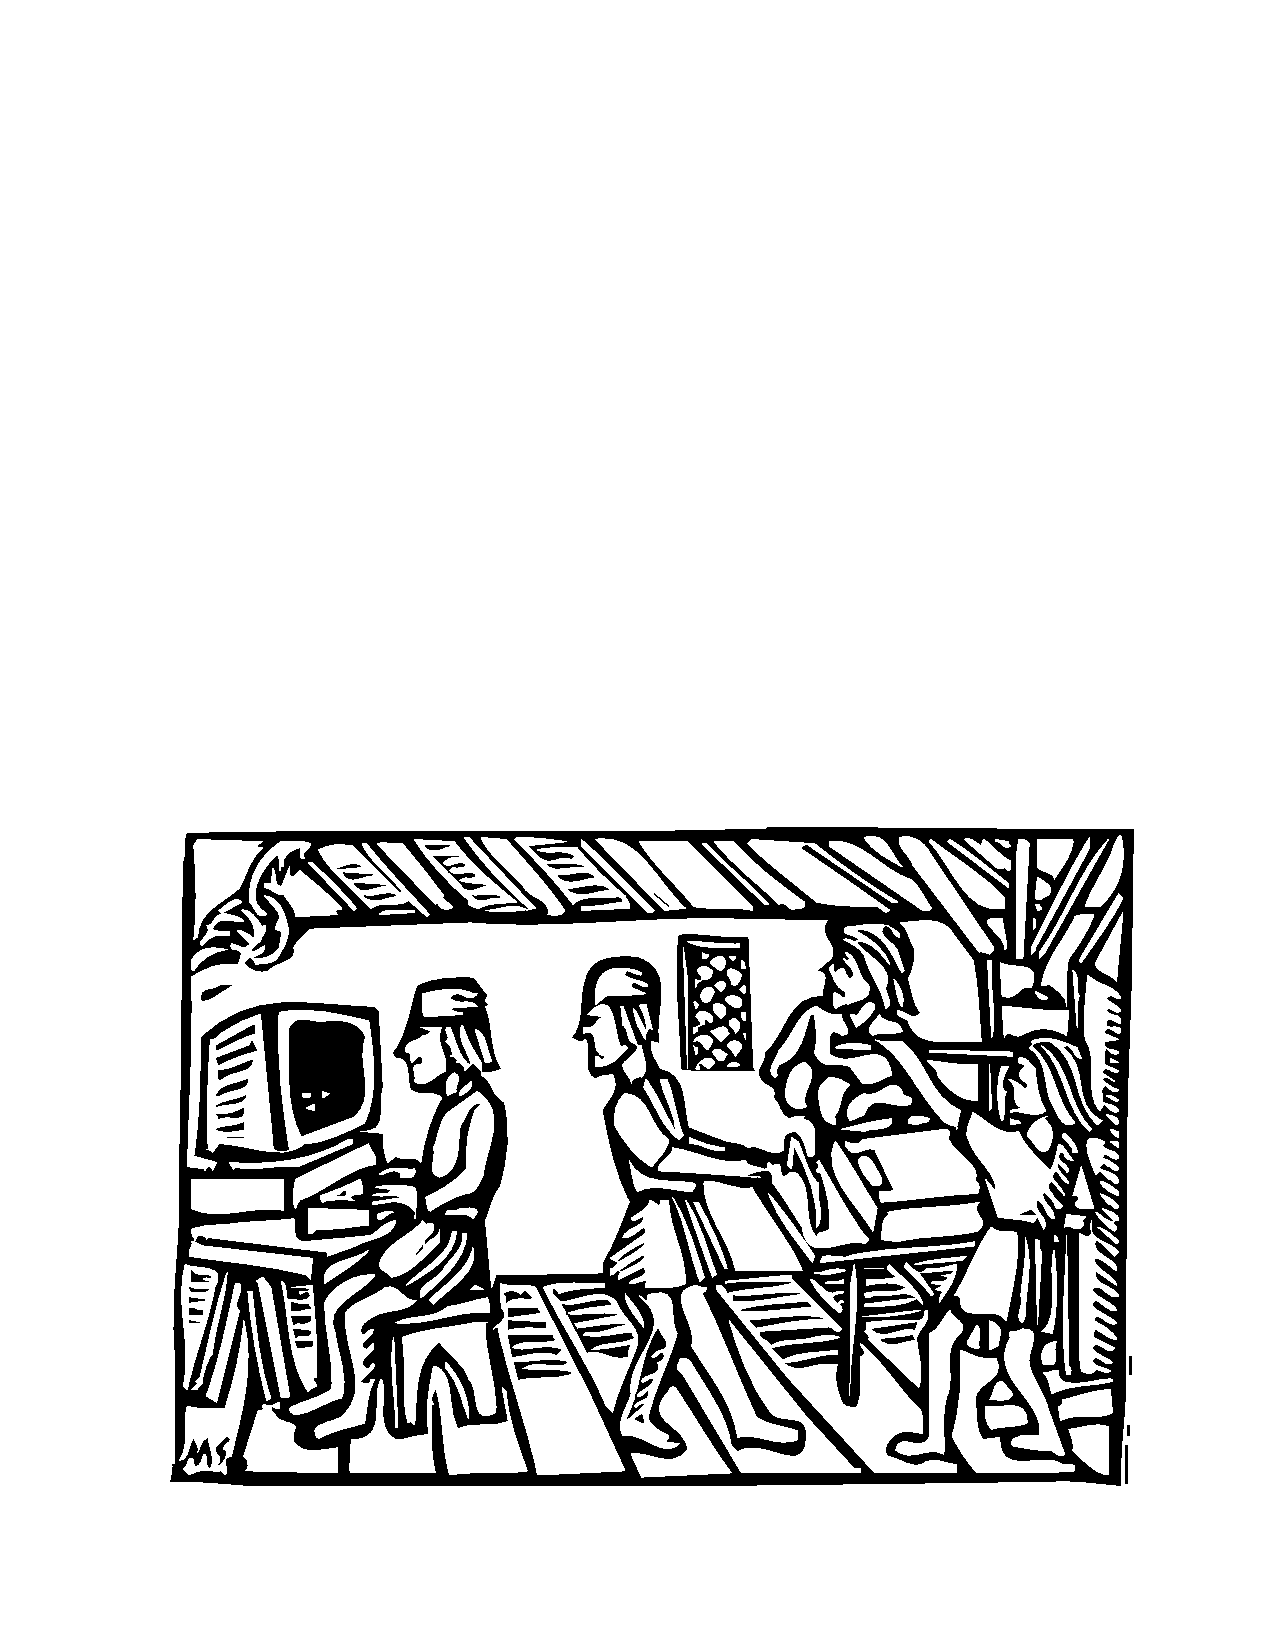
\includegraphics[width=.27\textwidth]{typography}} \qquad
\subfloat[]{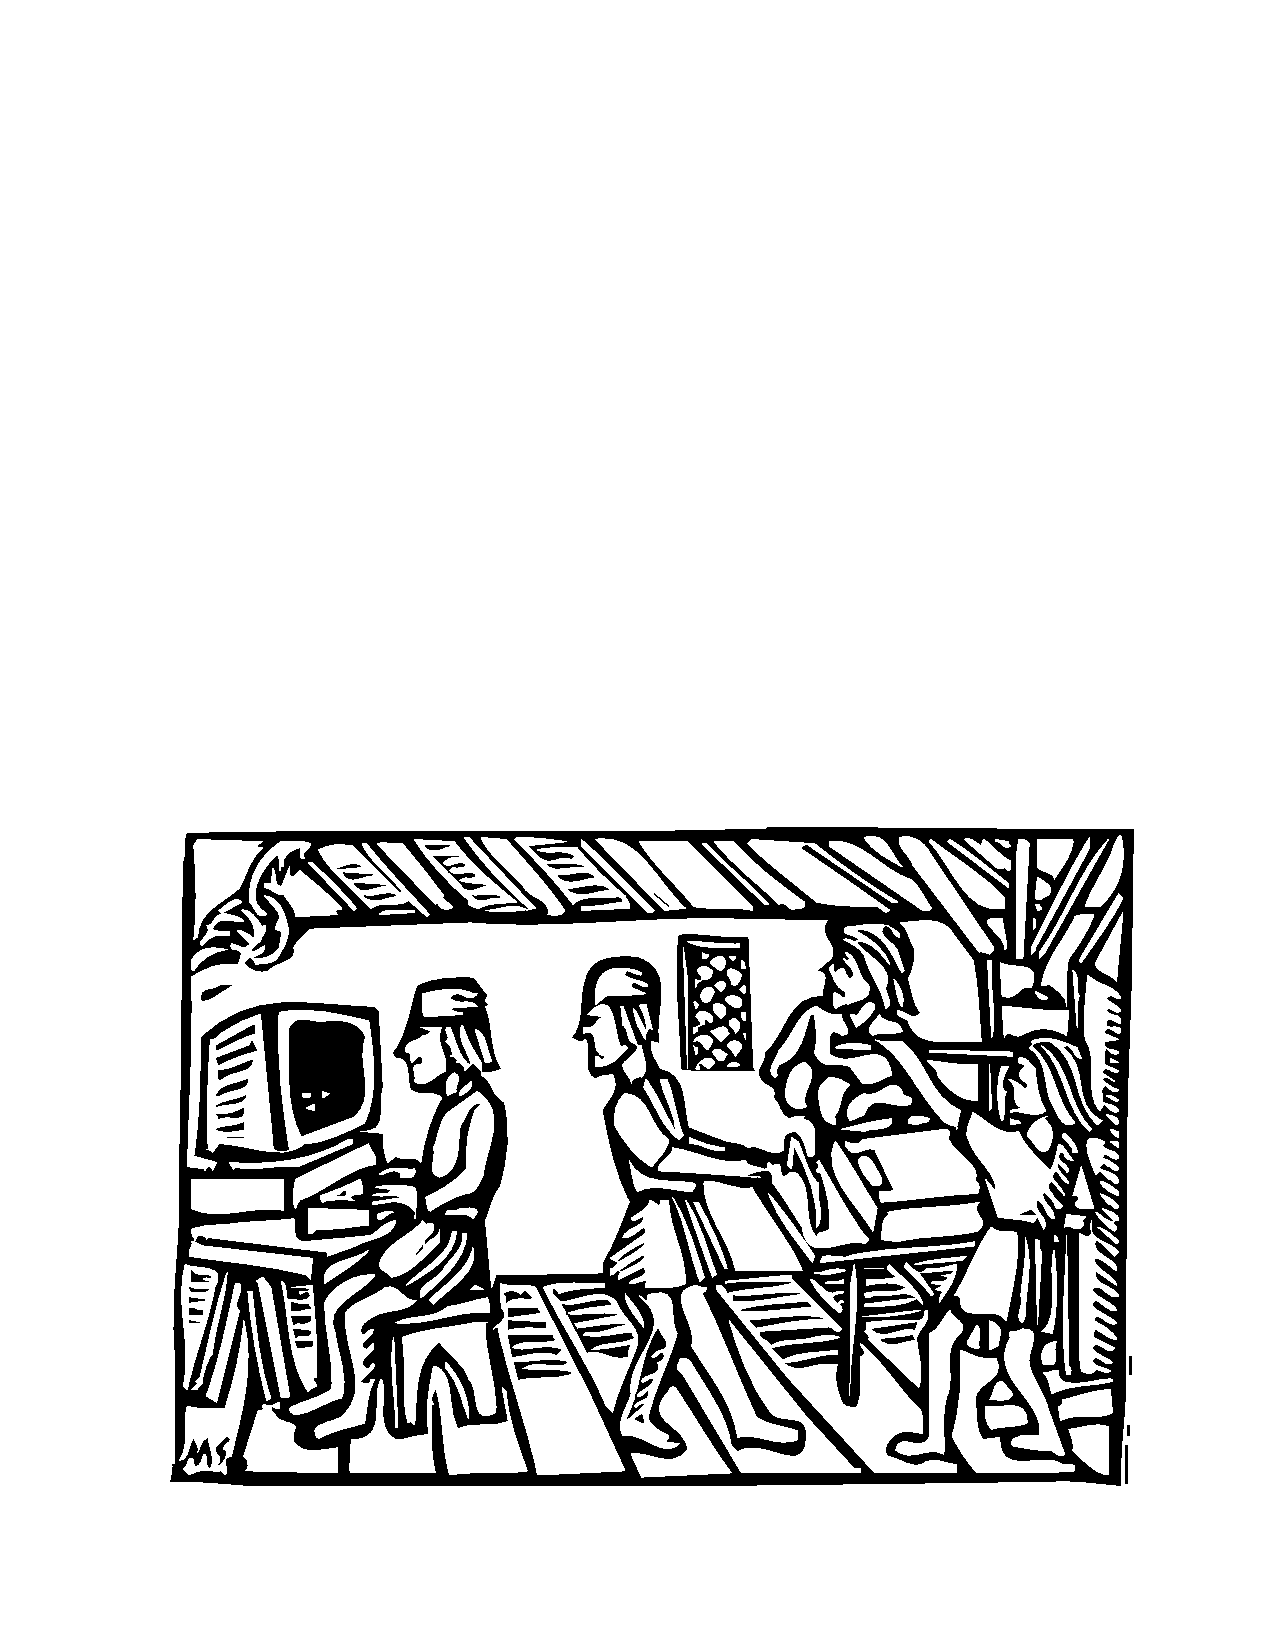
\includegraphics[width=.27\textwidth]{typography}}
\caption{并排图片}
\label{fig:subfig:3x2}
\end{figure}

要注意,图\ref{fig:subfig:3x2}例中
\texttt{qquad}相当于\verb|\hspace{2em}|,也就是2个字符的宽度,约0.08倍页宽,
图片宽度设定为0.27倍页宽是合适的;在该环境中,尽量不要手动换行,所以,不妨自己计算一下!

如果要把编号的两个图形并排,那么小页(minipage)就非常有用了,可以分别参考
图\ref{fig:parallel1}和图\ref{fig:parallel2}。其实这个例子和表格一节中并排
放置的表格一摸一样。
\begin{figure}[htb]
\begin{minipage}{0.48\textwidth}
  \centering
  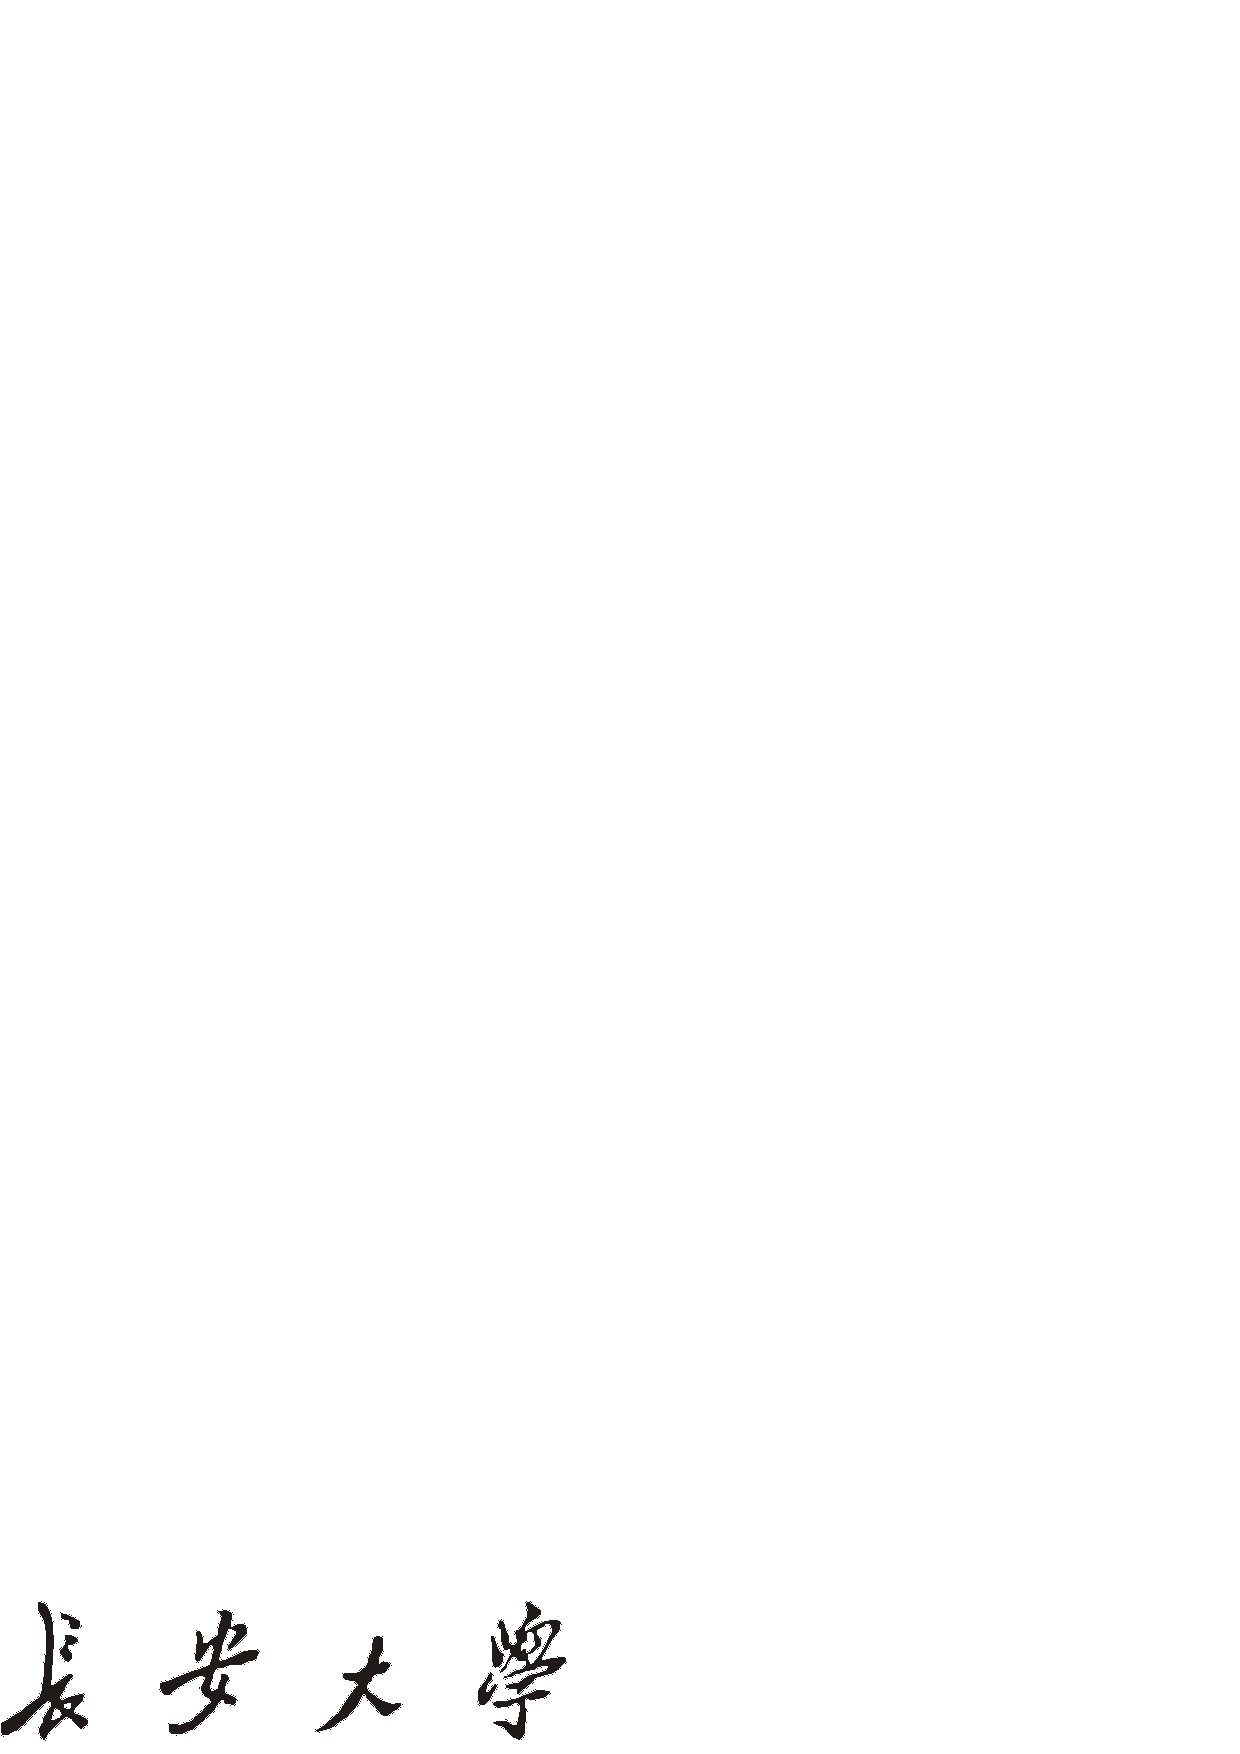
\includegraphics[height=1.2cm]{chdname.pdf}
  \caption{并排第一个图}
  \label{fig:parallel1}
\end{minipage}\hfill
\begin{minipage}{0.48\textwidth}
  \centering
  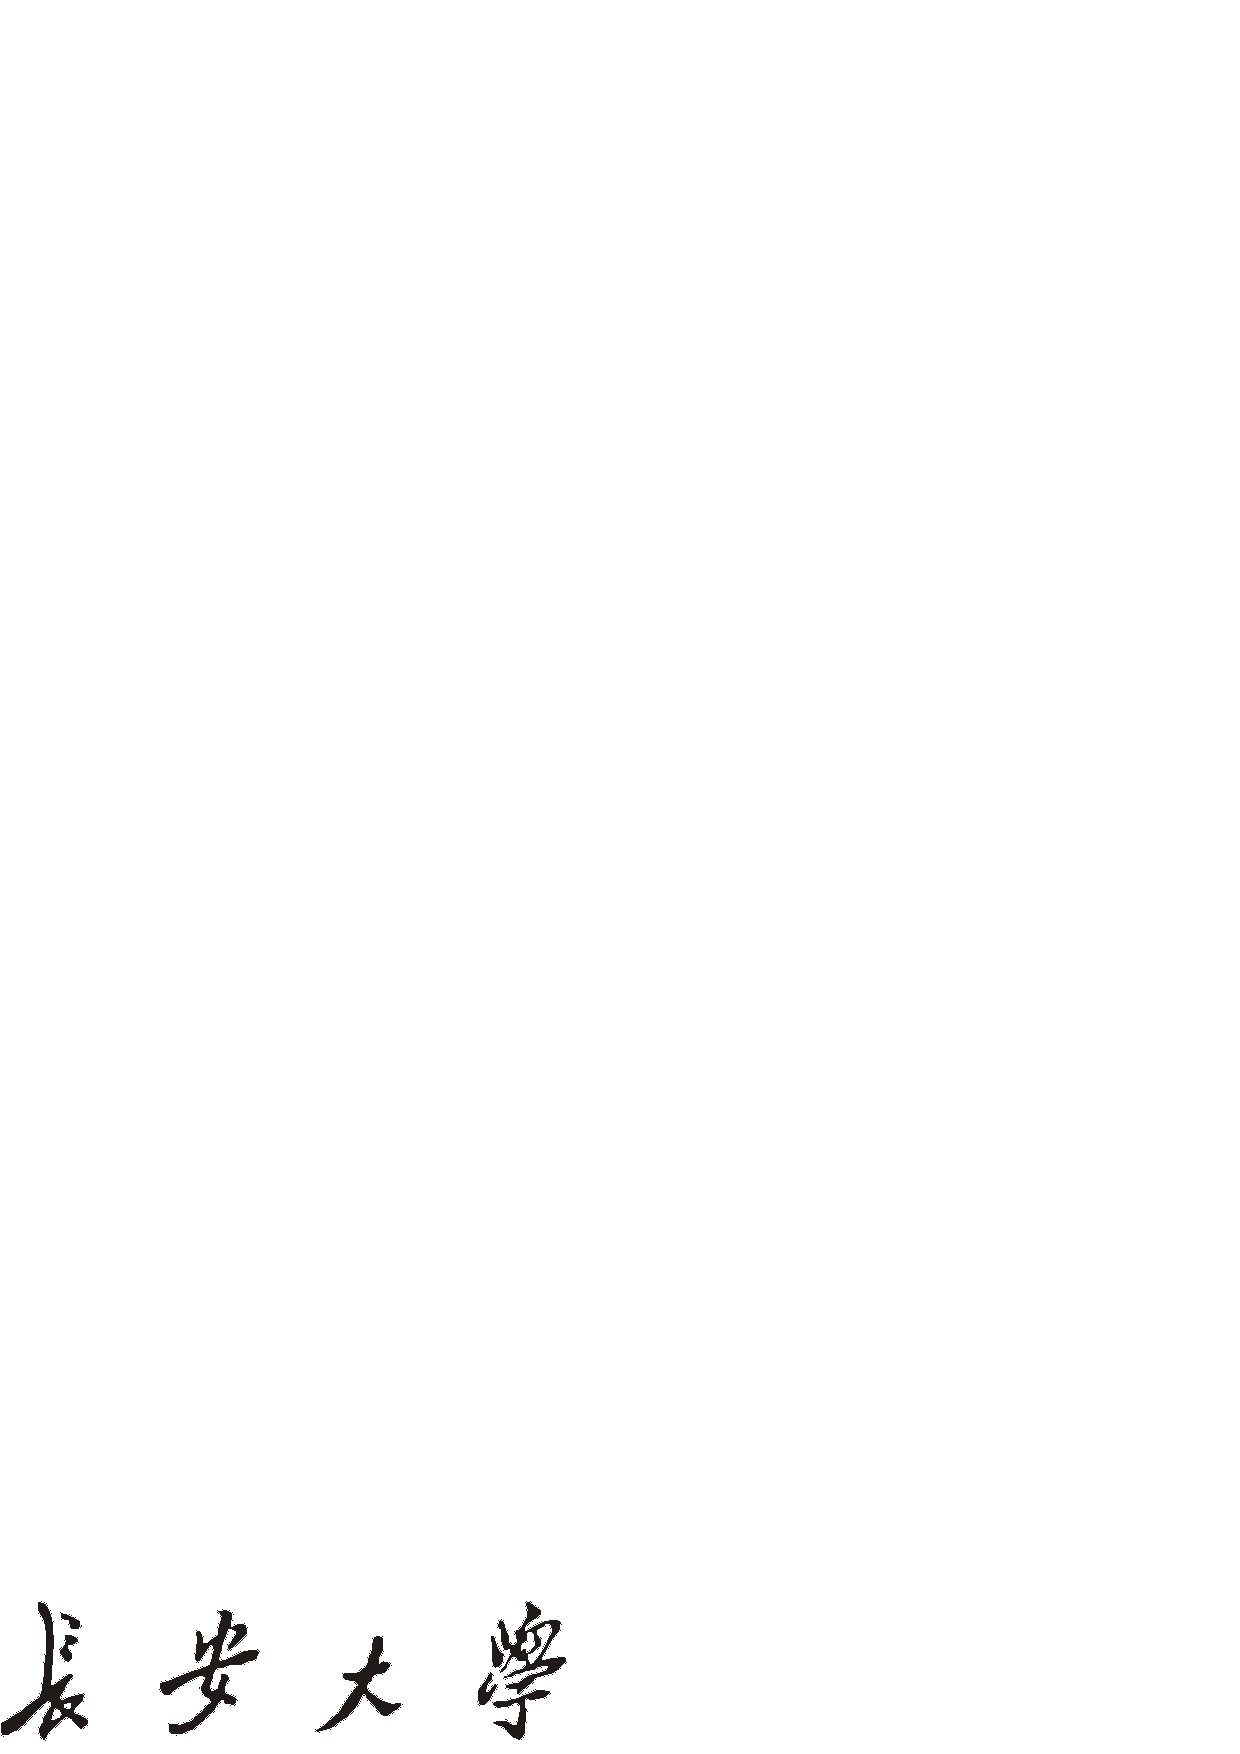
\includegraphics[height=1.2cm]{chdname.pdf}
  \caption{并排第二个图}
  \label{fig:parallel2}
\end{minipage}
\end{figure}

图形就说这么多,因为大家在写论文是遇到的最大问题不是怎么把图插进去,
而是怎样做出专业的、诡异的、震撼的图片来,记得在这时参考前面推荐的那
些工具吧,当然必不可少的是\Matlab{}了,至于如何加入中文标注、支持中文等等
可以上网去查,但这里{\kai 推荐一点},用好export命令,使得插入图片时尽可能的不要
缩放,保证图文的一致性。

\section{公式定理}
\label{sec:equation}
今有上禾三秉,中禾二秉,下禾一秉,实三十九斗;上禾
二秉,中禾三秉,下禾一秉,实三十四斗;上禾一秉,中禾二
秉,下禾三秉,实二十六斗。问上、中、下禾实一秉各几何?
\begin{align}
3x+2y+z &= 39\nonumber\\
2x+3y+z &= 34\nonumber\\
x+2y+3z &=26\nonumber
\end{align}

\zuozhe{《九章算术》}

贝叶斯公式如式 \eqref{equ:chap1:bayes},其中$p(y|\mathbf{x})$为后验;
$p(\mathbf{x})$为先验;分母$p(\mathbf{x})$ 为归一化因子,这是
实际应用中十分恐怖的一个积分式。
\begin{equation}
\label{equ:chap1:bayes}
p(y|\mathbf{x}) = \frac{p(\mathbf{x},y)}{p(\mathbf{x})}=
\frac{p(\mathbf{x}|y)p(y)}{p(\mathbf{x})}
\end{equation}

论文里面公式越多,\TeX{} 就越 happy。再看一个 \textsf{amsmath} 的例子:
\newcommand{\envert}[1]{\left\lvert#1\right\rvert}
\begin{equation}\label{detK2}
\det\mathbf{K}(t=1,t_1,\dots,t_n)=\sum_{I\in\mathbf{n}}(-1)^{\envert{I}}
\prod_{i\in I}t_i\prod_{j\in I}(D_j+\lambda_jt_j)\det\mathbf{A}
^{(\lambda)}(\overline{I}|\overline{I})=0.
\end{equation}

看看这个$\xLongrightarrow[to~love]{we~love}$,这个包的说明文件是doc文件夹中的\textsf{extarrows-test}文档

大家在写公式的时候一定要好好看doc文件夹中的\textbf{ChinaTeXMathFAQV1.1}文档,诸如多行公式环境,比如equarray,align 这些环境有哪些不同,使用上有哪些差异,我应该怎么调节公式才能得到更美观的公式等。

多多练习才是学习\LaTeX 公式排版的王道。

还有nicefrac宏包$\hat{\bm{x}}_k = \bm{x}_{\nicefrac{k}{k-1}}+\bm{K}_{UKF}(\bm{z}_k-\hat{\bm{z}}_{\nicefrac{k}{k-1}})$式 \eqref{equ:omegaik}中
\begin{equation}\label{equ:omegaik}
\bm{\omega}^i_{k}=\bm{\omega}^i_{k-1}\frac{\bm{p}(\left. \bm{z}_{k} \middle/ \bm{x}^i_{k} \right.)\bm{p}(\left. \bm{x}^i_{k} \middle/ \bm{x}^i_{k-1} \right.)}{\bm{q}(\left. \bm{x}^i_{k} \middle/ \bm{x}^i_{k-1},\bm{z}_k \right.)}
\end{equation}

分数线还可以长一些,如式 \ref{equ:oqzgyh},有没有发现此处的公式引用和上面的不一样呢,上面用的是\verb|\eqref{}|,而这里用的是\verb|\ref{}|
\begin{equation}\label{equ:oqzgyh}
\bm{\omega}^i_k = \bm{\omega}^i_k \Biggm/ \sum^n_{j=1}\bm{\omega}^j_k
\end{equation}
\begin{multline*}%\tag{[b]} % 这个出现在索引中的
\int_a^b\biggl\{\int_a^b[f(x)^2g(y)^2+f(y)^2g(x)^2]
 -2f(x)g(x)f(y)g(y)\,dx\biggr\}\,\mathrm{d}y \\
 =\int_a^b\biggl\{g(y)^2\int_a^bf^2+f(y)^2
  \int_a^b g^2-2f(y)g(y)\int_a^b fg\biggr\}\,\mathrm{d}y
\end{multline*}

再看\ref{equ:split}:
\begin{equation}\label{equ:split}
\begin{split}
C(z) &= [z^n] \biggl[\frac{e^{3/4}}{\sqrt{1-z}} +
e^{-3/4}(1-z)^{1/2} + \frac{e^{-3/4}}{4}(1-z)^{3/2}
+ O\Bigl( (1-z)^{5/2}\Bigr)\biggr] \\
&= \frac{e^{-3/4}}{\sqrt{\pi n}} - \frac{5e^{-3/4}}{8\sqrt{\pi
n^3}} + \frac{e^{-3/4}}{128 \sqrt{\pi n^5}} +
O\biggl(\frac{1}{\sqrt{\pi
n^7}}\biggr)
\end{split}
\end{equation}

当然了,数学中必不可少的是定理和证明。

定理定义[]中是可选参数,用来说明定理的名称。其他环境格式书写与上面定理、定义、推论格式相同,可自己调用其他环境。
若需要书写定理定义等内容,而且带有顺序编号,需要采用如下环境。除了~\verb|proof|~环境之外,其余13个环境都可以有一个可选参数作为附加标题。
\begin{center}
\vspace{0.5em}\noindent\wuhao\begin{tabularx}{0.7\textwidth}{lX|lX}
性质 & \verb|character|~环境 & 引理 & \verb|lemma|~环境 \\
定理 & \verb|theorem|~环境 & 公理 & \verb|axiom|~环境 \\
猜想 & \verb|conjecture|~环境 & 命题 & \verb|proposition|~环境 \\
练习 & \verb|exercise|~环境 & 例 & \verb|example|~环境 \\
问题 & \verb|problem|~环境 & 注释 & \verb|remark|~环境 \\
推论 & \verb|corollary|~环境 & 证明 & \verb|proof|~环境 \\
假设 & \verb|assumption|~环境 & 定义 & \verb|definition|~环境 \\
\end{tabularx}
\end{center}
\begin{definition}[谱半径]\label{def:def1}
称$n$阶方阵$\mathbf{A}$的全体特征值
$\lambda_1,\cdots,\lambda_n$组成的集合为$\mathbf{A}$的谱,称
$$\rho(\mathbf{A})=\max{\{|\lambda_1|,\cdots,|\lambda_n|\}}$$
\end{definition}
\begin{theorem}[相似充要条件]\label{lemma:l1}
方阵$A$和$B$相似的充要条件是:$A$和$B$有全同的不变因子。
\end{theorem}
\begin{corollary}[推论1]\label{cor:cor1}
在赋范空间$(X,\|\cdot\|)$上定义$d(x,y)=\|x-y\|$,
对任意$x,y\in X$,则$(X,d)$是距离空间。
\end{corollary}
\begin{proof}
只需证明$d(x,y)$是距离。
\end{proof}
\begin{theorem}
  \label{chapTSthm:rayleigh solution}
  假定 $X$ 的二阶矩存在:
  \begin{equation}
         O_R(\mathbf{x},F)=\sqrt{\frac{\mathbf{u}_1^T\mathbf{A}\mathbf{u}_1} {\mathbf{u}_1^T\mathbf{B}\mathbf{u}_1}}=\sqrt{\lambda_1},
  \end{equation}
  其中 $\mathbf{A}$ 等于 $(\mathbf{x}-EX)(\mathbf{x}-EX)^T$,$\mathbf{B}$ 表示协方差阵 $E(X-EX)(X-EX)^T$,$\lambda_1$
$\mathbf{u}_1$是$\lambda_1$对应的特征向量,
\end{theorem}

对于希腊符号使用\verb|mathbf|命令可能有些问题,所以建议对符号
用\verb|bm|加粗,记得用\verb|\up<greek>|切换正体符号,下面看几个例子:
\verb|\gamma|斜体代表变量$\gamma$,\verb|\bm{\upgamma}|正体代表向量$\bm{\upgamma}$,
。\verb|\Gamma|正体代表操作符号$\Gamma$,
\verb|\bm{\Gamma}|正体粗体代表矩阵形式$\bm{\Gamma}$,
\verb|\varGamma|斜体代表变量$\varGamma$。另外对于大小写斜体的加粗可以见$\bm{\gamma}$和$\bm{\varGamma}$,
但是这两种科技论文中很少出现,这里只做测试。
非符号普通向量就用\verb|\mathbf|吧:$\mathbf{x}_k,\mathbf{X}_k$。
完整测试如下$\omega,\bm{\omega},\upomega,\bm{\upomega},\Omega,\bm{\Omega},\varOmega,\bm{\varOmega}$。

\begin{proof}
上述优化问题显然是一个Rayleigh商问题。我们有
  \begin{align}
     O_R(\mathbf{x},F)=\sqrt{\frac{\mathbf{u}_1^T\mathbf{A}\mathbf{u}_1} {\mathbf{u}_1^T\mathbf{B}\mathbf{u}_1}}=\sqrt{\lambda_1},
 \end{align}
 其中 $\lambda_1$ 下列广义特征值问题的最大特征值:
$$
\mathbf{A}\mathbf{z}=\lambda\mathbf{B}\mathbf{z}, \mathbf{z}\neq 0.
$$
 $\mathbf{u}_1$ 是 $\lambda_1$对应的特征向量。结论成立。
\end{proof}

下面来看看算法环境的定义和使用。
我们知道,故障诊断的最终目的,是将故障定位到部件,而由于信号--部件依赖矩阵的存在,因此,实质性的工作是找出由故障部件发出异常信号,
不妨称为源异常信号,而如前所述,源异常信号与异常信号依赖矩阵$\mathbf{S_a}$的全零列是存在一一对应的关系的。因此,我们只要获得了$\mathbf{S_a}$的全零列的相关信息,
也就获得了源异常信号的信息,从而能进一步找到故障源。
通过以上分析,我们构造算法\ref{alg53},用于实现非回路故障诊断。
\begin{algorithm}[htbp]
  \caption{非回路故障诊断算法}
  \label{alg53}
  \begin{algorithmic}[1]
    \REQUIRE 信号--部件依赖矩阵$\mathbf{A}$,信号依赖矩阵$\mathbf{S}$,信号状态向量$\alpha$
    \ENSURE 部件状态向量$\gamma$
    \STATE $\mathbf{P}\leftarrow\left(<\alpha>\right)$
    \STATE $\mathbf{S_{a}}\leftarrow\mathbf{P^T}\mathbf{S}\mathbf{P}$
    \FOR{$i=1$ to $S_a$的阶数$m$}
    \STATE $s_i\leftarrow s_i$的第$i$个行向量
    \ENDFOR
    \STATE $\beta_a\leftarrow\lnot \left(s_1\lor s_2\lor \cdots\lor s_m\right)^T$
    \STATE $\beta\leftarrow\mathbf{P}\beta_a$
    \STATE $\gamma\leftarrow\mathbf{A}\beta$
  \end{algorithmic}
\end{algorithm}

第一类故障回路推理与非回路故障推理是算法基本相同,稍微不同的是$\beta_a$的计算。因为第一类故障回路中的信号全部可能是源异常信号,因此我们不必计算
$\beta_a=\lnot \left(\left[s_1\lor s_2\lor \cdots\lor s_m\right]^T\right)$,而直接取$\beta_a=\left[\underbrace{\begin{array}{cccc}1&1&\cdots&1\end{array}}_m\right]^T$,将$\beta_a$代入
算法\ref{alg53},有
\[\beta=\mathbf{P}\beta_a=\mathbf{P}\underbrace{\left[\begin{array}{cccc}1&1&\cdots&1\end{array}\right]^T}_m=\alpha\]
因此一类故障回路的推理算法变得相当简单,例如算法\ref{alg54}
\begin{algorithm}[htbp]
  \caption{第一类故障回路诊断算法}
  \label{alg54}
  \begin{algorithmic}[1]
    \REQUIRE 信号--部件依赖矩阵$\mathbf{A}$,信号状态向量$\alpha$
    \ENSURE 部件状态向量$\gamma$
    \STATE $\gamma\leftarrow\mathbf{A}\alpha$
  \end{algorithmic}
\end{algorithm}

\section{参考文献}
\label{sec:bib}
当然参考文献可以直接写 bibitem,虽然费点功夫,但是好控制,各种格式可以自己随意改
写,在chdpaper里面,建议使用JabRef编辑和管理文献,再结合\verb|bstutf8.bst|,
对中文的支持非常不错,格式也很规范。

本模板推荐使用 BIB\TeX,样式文件为 bstutf8.bst,符合学校的参考文献格式(如上标引用的括号为中文中括号【】)。由于学校的要求比较怪,是中文中括号。为了解决这个问题我把natbib.sty宏包给修改了,并将其存储为UTF-8的格式才成功,修改后的宏包已经与模板放在一起,直接使用即可。看看这个例子,关于书的\upcite{tex, companion},
还有这些\upcite{Krasnogor2004e, zjsw},关于杂志的\upcite{ELIDRISSI94,
  MELLINGER96, SHELL02},硕士论文\upcite{zhubajie, metamori2004},博士论文\upcite{shaheshang, FistSystem01},标准文件\upcite{IEEE-1363},会议论文\upcite{DPMG,kocher99},%
技术报告\upcite{NPB2}。中文参考文献\upcite{cnarticle}\textsf{特别注意},需要在\verb|bibitem|中
增加\verb|language|域并设为\verb|zh|,英文此项可不填,之后由\verb|bstutf8|统一处理
(具体就是决定一些文献在中英文不同环境下的显示格式,如等、etc)。
若使用\verb|JabRef|,则你可按下面步骤来设置:
选择\textsf{Options}$\rightarrow$\textsf{Set Up General Fields},
在\verb|General:|后加入\verb|language|就可以了。

有时候不想要上标,那么可以这样\cite{shaheshang},这个非常重要。但是这个间距有点大,暂时还没想到好的办法。学校也没要求用这样的格式,所以先不管了。
\subsection{参考文献生成方法}

\LaTeX~具有插入参考文献的能力。Google Scholar~网站上存在兼容~BibTeX~的参考文献信息,通过以下几个步骤,可以轻松完成参考文献的生成。
\begin{itemize}
  \item 在\href{http://scholar.google.com/}{\underline{谷歌学术搜索}}中,
        点击\href{http://scholar.google.com/scholar_preferences?hl=en&as_sdt=0,5}{\underline{学术搜索设置}}。
  \item 页面打开之后,在\textbf{文献管理软件}选项中选择\textbf{显示导入~BibTeX~的链接},单击保存设置,退出。
  \item 在{\lishu 谷歌学术}搜索中检索到文献后,在文献条目区域单击导入BibTeX选项,页面中出现文献的引用信息。
  \item 将文献引用信息的内容复制之后,添加到ref文件夹下的refs.bib中。
\end{itemize}

在正文中标注参考文献时,在需要标注的地方输入\verb|\upcite{}|指令,花括号
内输入参考文献引用信息中的第一行信息即可(常常为文献的缩略信息),如
\autoref{fig:ref}红线所圈小括号内部分。

在下载\href{http://jabref.sourceforge.net/documentation.php}{\underline{这里}}JabRef最新版,安装前先下载
jre环境。
\begin{figure}[htp]
\centering
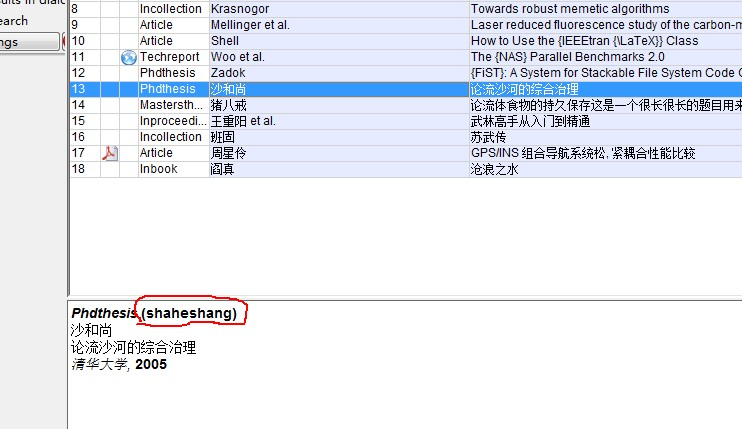
\includegraphics[width=0.7\textwidth]{ref.jpg}
\caption{JabRef2.4打开.bib文件}
\label{fig:ref}
\end{figure}
\section{代码高亮}
有些时候我们需要在论文中引入一段代码,用来衬托正文的内容,或者体现关键思路的实现\upcite{cnproceed}。
在模板中,统一使用\texttt{listings}宏包,并且设置了基本的内容格式,并建议用户只
使用三个接口,分别控制:编程语言,行号以及边框。简洁达意即可,下面分别举例说明。

首先是设定语言,来一个C的,使用的是默认设置:
\begin{lstlisting}[language=C]
void sort(int arr[], int beg, int end)
{
  if (end > beg + 1)
  {
    int piv = arr[beg], l = beg + 1, r = end;
    while (l < r)
    {
      if (arr[l] <= piv)
        l++;
      else
        swap(&arr[l], &arr[--r]);
    }
    swap(&arr[--l], &arr[beg]);
    sort(arr, beg, l);
    sort(arr, r, end);
  }
}
\end{lstlisting}

当我们需要高亮Java代码,不需要行号,不需要边框时,可以:
\begin{lstlisting}[language=Java,numbers=none,frame=none]
// A program to display the message
// "Hello World!" on standard output 这是中文
// 这是中文 a+b=c

public class HelloWorld {

   public static void main(String[] args) {
      System.out.println("Hello World!");
   }

}   // end of class HelloWorld
\end{lstlisting}

细心的用户可能发现,行号被放在了正文框之外,事实上这样是比较美观的,
如果有些用户希望在正文框架之内布置所有内容,可以:
\begin{lstlisting}[language=perl,xleftmargin=2em,framexleftmargin=1.5em]
#!/usr/bin/perl
print "Hello, world!\n";
\end{lstlisting}

好了,就这么多,\texttt{listings}宏包的功能很强大也很复杂,如果需要自己定制,
可以查看其手册,耐心阅读总会找到答案。
\textbf{注意:} 当前代码环境中文注释的处理还不是很完善,对于注释请妥善处理。
在本模板中,推荐算法环境或者去掉中文的listings代码环境。
如果需要包含中文注释,不要求代码高亮,
就用\texttt{code}环境,这个环境是Verbatim的定制版,简单有效,
调用的是fancyvbr宏包,用户可在mynudt.sty中修改它的外观等等。
这里我们还可以给代码加上标签。
\begin{code}[label=hello.c]
public class HelloWorld {
   public static void main(String[] args) {
      System.out.println("Hello World!");
   }
}   // 世界,你好!
\end{code}

\section{符号列表}{(我们学校没有要求这个,我就把这个删掉了,如果要,可以参考nudtpaper.thesis)}

{\hei 前面的话:}{\kai\color{blue}
2.2版本后默认使用nomencl环境,如果你还是希望使用传统的\verb|definition.tex|,那么只需注释掉
顶层文件中的nomenclature即可。}

符号列表使用的是\verb|nomencl|包,自己简单定制了下,使用方法分为四步:
\begin{compactenum}
\item 将\verb|\makenomenclature|语句放在正文前,即\verb|\begin{document}|前面;
\item 将\verb|\printnomenclature|放在论文中,我在例子中将符号列表放在了英文摘要的
后面,正文第一章的前面,当然,你可以根据自己的需要或者教研室的规范放置在合理的位置上,
为了页面引用的正确,在这句话前面放上\verb|\cleardoublepage|;
\item 使用\verb|\nomenclature|命令在论文的各个位置上添加符号定义,语法后面会讲到;
\item 编译。编译需要首先运行一遍xelatex,之后运行
\begin{code}
makeindex -s nomencl.ist -o thesis.nls thesis.nlo
\end{code}
\end{compactenum}

你可以把这句编译命令放在\verb|makepdf.bat|中第一个\verb|xelatex thesis|下面。然后
双击\verb|makepdf.bat|就可以了,论文模板中已经为你添加上了,如果你强烈不想使用
nomencl环境,只要把它注释掉(前面加\verb|rem|)就可以。
另外,由于我使用的是VIM来编辑\TeX{}代码,具体到每个编辑器(诸如WinEDT,TeXWorks等)
如何设定该命令的快捷按钮,诸位可以搜索网上的教程。

下面简单说明下\verb|\nomenclature|命令,语法为。这里插入一些随机的文字,希望
对你在阅读帮助中的思维没有什么不良的影响。
\begin{code}
\nomenclature[<prefix>]{<symbol>}{<desc>}{<null>}
\end{code}
\verb|nomencl|模板的默认排序方法可能(大多都)不满足要求,
论文模板里,我们通过设定\verb|<prefix>|来实现符号列表的排序。
它分为两部分,比如如\verb|[Aa]|,第一个字母的含义是:
\begin{compactitem}
\item[`A'] 符号归为拉丁字母
\item[`G'] 希腊字母
\item[`X'] 上标
\item[`Z'] 下标
\end{compactitem}
每个标识后边的字幕\verb|a-z|作为当前符号组内的排列顺序,比如$\beta$就可以写成
\verb|[Gb]|,诸如此类。当然你一定注意到了,这个排序分组的设定只是为了记忆
方便,并不是强制的,因此你可以有自己的方案,比如Z是Greek,
R是Roman什么的,只要统一就好,只需记住,组间排列是按字母顺序排的。

注意符号表分四列,前三列的含义与命令中相同,
最后一列是符号定义时所在的页码。效果看例子,对于下式:
\begin{equation}\label{eq:heatflux}
   \dot{Q} = k \cdot A \cdot \Delta T
\end{equation}%
\nomenclature[Aq]{$\dot{Q}$}{heat flux}{}%
\nomenclature[Ak]{$k$}{overall heat transfer coefficient,式\eqref{eq:ohtc}}{}%
\nomenclature[Aa]{$A$}{area}{}%
\nomenclature[Al]{$L$}{length}{}%
\nomenclature[At]{$T$}{temperature}{}%
\nomenclature[At]{$\Delta T$}{temperature difference}{}%
\nomenclature[Gr]{$\gamma$}{中文测试, 以及一句很长的物理意义,很有可能超过当前栏的宽度,主要目的是看一看会不会出现某些异常情况。}{}%

或者:
\begin{equation}\label{eq:ohtc}
    \frac{1}{k} = \left[\frac{1}{\alpha _{\mathrm{i}}\,r_{\mathrm{i}}} +
    \sum^n_{j=1}\frac{1}{\lambda _j}\,
    \ln \frac{r_{\mathrm{a},j}}{r_{\mathrm{i},j}} +
    \frac{1}{\alpha _{\mathrm{a}}\,
    r_{\mathrm{a}}}\right] \cdot r_{\mathrm{reference}}
\end{equation}%
\nomenclature[Ga]{$\alpha$}{convection heat transfer coefficient}{}%
\nomenclature[Zi]{i}{in}{}%
\nomenclature[Gl]{$\lambda$}{thermal conductivity}{}%
\nomenclature[Za]{a}{out}{}%
\nomenclature[Zn]{$n$}{number of walls}{}%
\nomenclature[Zj]{$j$}{running parameter}{}%

{\hei 注意事项:}{\kai 模板中定制的nomencl格式在mynudt.sty中,默认是三栏的,分别是:
``符号'',``定义'',``首次出现页码'',
注意这里的符号列表都没有单位,如果你需要额外的栏输入单位(呵呵,聪明的读者可能看出来
了,\verb|nomenclature|命令最后一个是空的,就是用来让你赋予她各种意义的)。
此时就需要你有一点点动手能力了(其实只要会修改表格就行),
方法很简单,比如需要添加``国际单位制''这一栏,则
\begin{compactenum}
\item 论文中\verb|\nomenclature|命令的第三个参数就让他代表单位,也可留空;
\item 将\verb|mynudt.sty|中longtable的表头添加``国际单位制''几个字,
你也可以取其他的名字,放在那个{\kai 应该出现的}位置上;
\item 由于增加了5个字,就把前面栏的宽度数字减5,同时设定第三栏宽度为5,
注意这一步需要你自己调整,记得不要让表格超出边界就行。
\end{compactenum}
}

\section{中文习惯}
\label{sec:chinese}

对于itemize及enumerate过大的行间距,我已经在\verb|mychd.sty|中重新修正。但是不一定满足每个人的要求,通过调用enumitem宏包可以很方便地控制罗列环境的布局,其\verb|mychd.sty|文件中的\verb|\setitemize|和\verb|\setenumerate|命令分别用来设置itemize和enumerate环境的样式参数。用户可以参考\autoref{fig:list}对这两种罗列环境的样式参数进行设定,也可以使用compactitem或本人在\verb|mychd.sty|中定义的myList环境来替代,但是模板中不进行默认替代,因为只有用户真正发现列表不好看才会找到这里,而且在示例文件中,陈赓大将那个列表环境如果压缩了行距会很不好看。
\begin{figure}[htp]
\centering
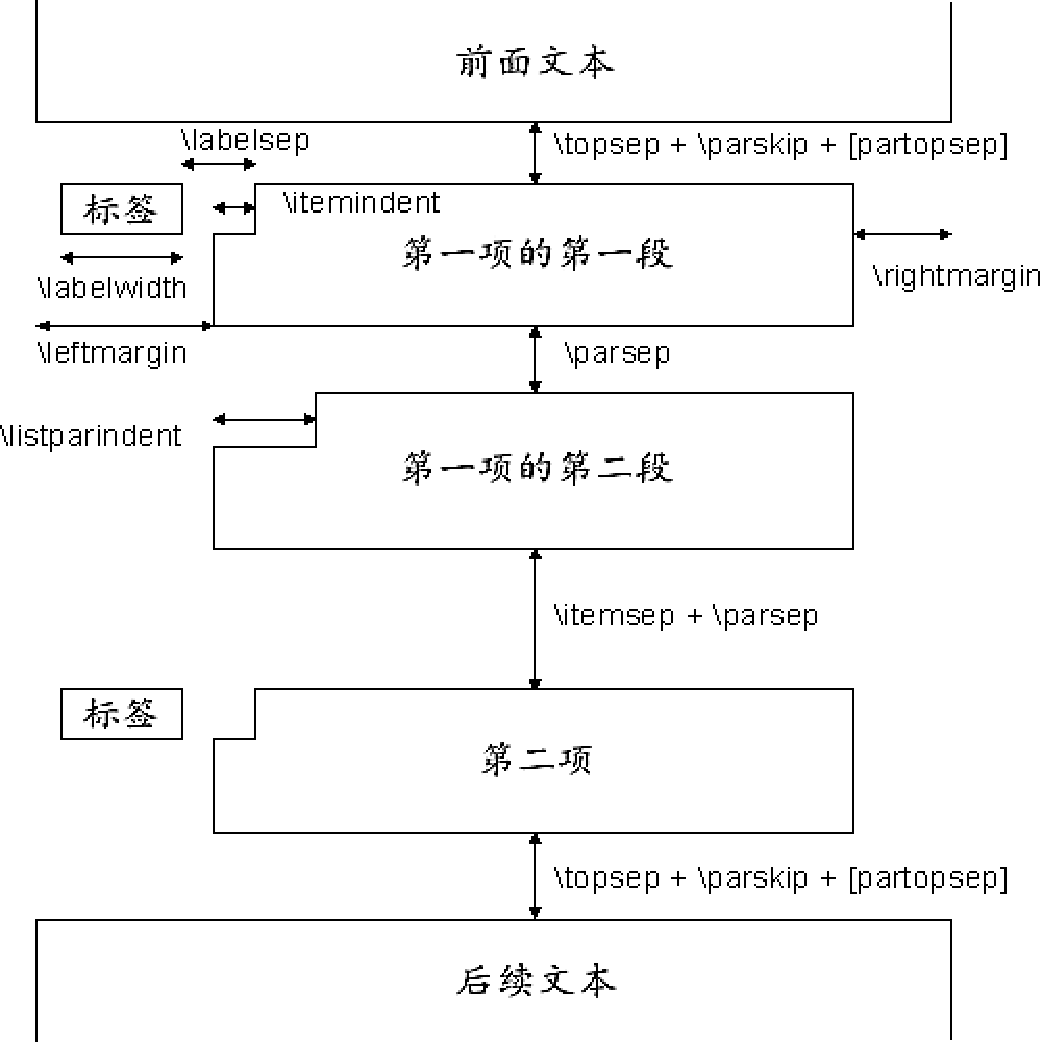
\includegraphics[width=0.7\textwidth]{list.pdf}
\caption{罗列环境参数示意图}
\label{fig:list}
\end{figure}

{\hei 一个重要的提示:}
作者自己的定义命令、包等,不要放在模板里面,请放到\verb|mychd.sty|
中,这样更新模板时,只要覆盖\verb|chdpaper.cls|即可。

中文破折号为一个两个字宽垂直居中的直线,输入法直接得到的破折号有时是两个断开的小短线
(——),有时不是,如果是的话,这看起来不舒服。所以模板中定义了一个破折号的命令 \verb|\pozhehao|,请看:

\mingyan{弘毅明德,笃学创新}{长安大学校训}
\section{如何查找说明文档}
附带说一个问题: 如何查找说明文档?
 \begin{enumerate}
    \item 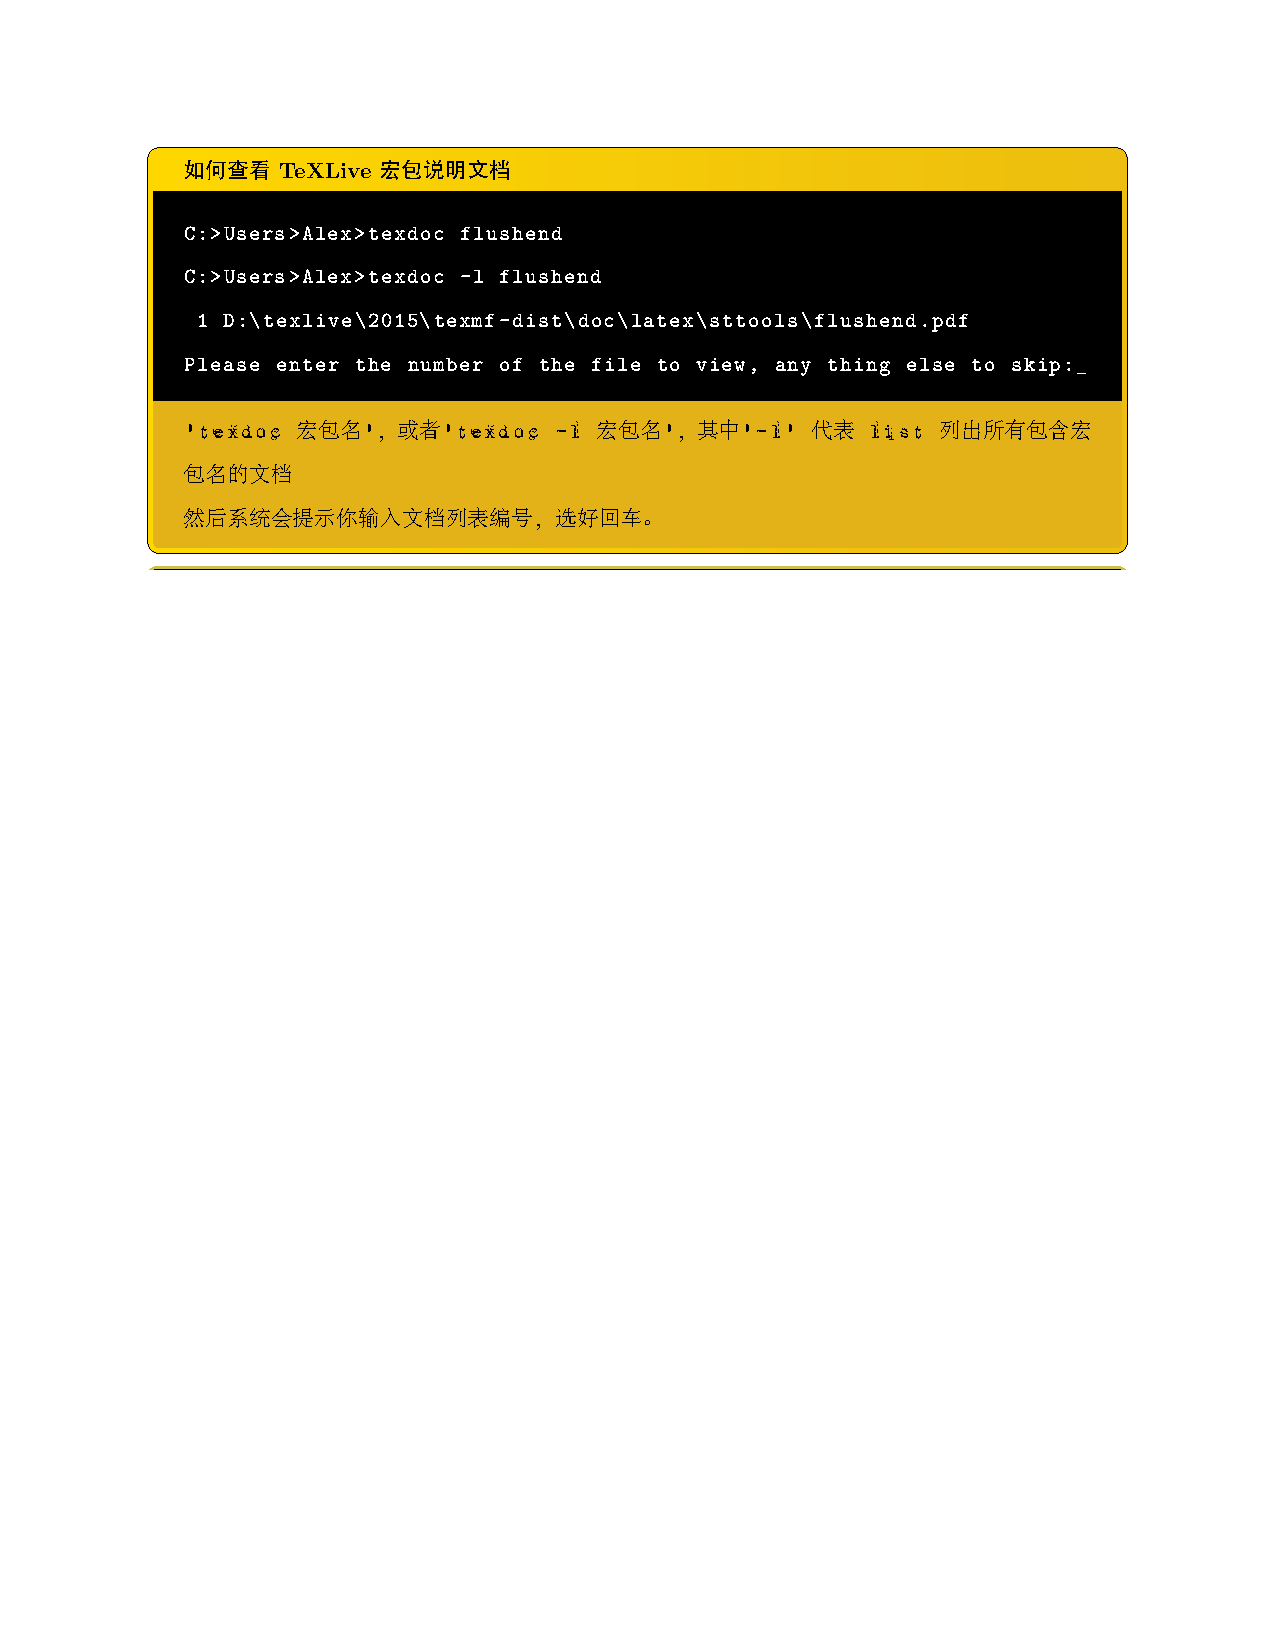
\includegraphics[width=0.6\textwidth]{helpdoc.PDF}
    \item 有时间的话, 自己到安装目录下去翻看吧, 里面有无尽的宝藏.
    \item 使用万能的~Google.
\end{enumerate}
%第二章
% !Mode:: "TeX:UTF-8"
%%% Local Variables:
%%% mode: latex
%%% TeX-master: "../main"
%%% End:

\begin{conclusion}
该部分主要包括两部分:“结论”和“展望”。结论是理论分析和实验结果的逻辑发
展,是整篇论文的归宿。结论是在理论分析、试验结果的基础上,经过分析、推理、判
断、归纳的过程而形成的总观点。结论必须完整、准确、鲜明、并突出与前人不同的新
见解。总结部分还应说明论文中的创新点内容。创新点应该以分条列举的形式进行提
出。展望是对该研究课题存在的不足和有待改进的说明,是对未来研究的一种期待。该
部分的字数应不少于半页\upcite{ELIDRISSI94,
  MELLINGER96, SHELL02}。
这里测试下myList环境:
\begin{myList}
        \item 封面;
        \item 毕业论文(设计)任务书;
        \item 开题报告;
        \item 中英文摘要及关键词
        \item  目录;
        \item  正文;
        \item  致谢
        \item  参考文献或资料;
        \item  附录(包括计算程序及说明、过长的公式推导等);
        \item  附件(包括图纸、外文文献\upcite{ELIDRISSI94}译文等);
\end{myList}

请直接单面打印PDF文件,空白页已经按要求留出。打印时,缩放页面的选项设
为“无”,否则页面会缩小。
\end{conclusion}%结论以及展望
% !Mode:: "TeX:UTF-8"
%%% Local Variables:
%%% mode: latex
%%% TeX-master: "../main"
%%% End:

\begin{thanks}
长安大学本科生毕业论文\XeLaTeX{}模板主要参考以下内容:
\begin{itemize}
\item 国防科技大学学位论文nudtpaper研究生学位论文\LaTeX{}模板大部
\item 天津大学TJUThesis本科毕业论文模板任务书,开题报告部分,书签以及目录部分titlerule的制作
\item 中国矿业大学硕博毕业论文\LaTeX{}模板cumtthesis封面部分
\item 东南大学学位论文\LaTeX{}模板seuthesis的logo制作以及pdf文档属性说明的设置
\item 人大微观经济学初等笔记扉页版本信息制作
\item 清华大学学位论文模板ThuThesis章节标题英文字体改为{\sffamily Arial},定理正文字体改为宋体,确实好看了不少,附件部分是引用薛同学的
\item 在\Chdpaper~v1.1将图表标题改为{\heiti 中文黑体}{\sffamily English Arial},以与章节标题统一
\end{itemize}

感谢$\mathbb{C}$\TeX{}论坛。

\bigskip
谨将此论文模板,献给我们最爱的母校:长安大学。

衷心感谢导师 xxx 老师对本人的精心指导。他们的言传身教将使我终生受益。

感谢\Chdpaper{},它的存在让我的论文写作轻松自在了许多,让我的论文格式规整漂亮了许多。

\end{thanks}
%致谢

\cleardoublepage
\phantomsection
\addcontentsline{toc}{chapter}{参考文献}
\bibliographystyle{gbt-7714-2015-numerical}
\bibliography{ref/refs}%参考文献

% 最后,需要的话还要生成附录,全文随之结束。

\appendix
\backmatter%附录
% TeX
%\chapter{部分仿真程序}
\chapter{部分仿真程序}\label{ch:fz}
\lstset{% general command to set parameter(s)
basicstyle=\ttfamily\small, % print whole listing small
keywordstyle=\color{black}\bfseries,
% \underbar underlined bold black keywords
identifierstyle=, % nothing happens
commentstyle=\color{black}, % white comments
%stringstyle=\ttfamily, % typewriter type for strings
showstringspaces=false, % no special string spaces
stepnumber=2}
\begin{lstlisting}[language=Matlab,caption={最小二乘法获取系统传递函数}]
%%
% 输入参数:
% x  ---  系统输入阵列
% y  ---  系统输出阵列
% N  ---  系统传递函数的阶数
% 函数输出:
% 系统 Z 传递函数分子与分母的系数,即: h(z) = numd(z) / dend(z)

%%

function [numd, dend] = LeastSquare(x, y, N)
count = length(y);
M = count - 1;
ai = zeros(N*2, M);
for i=1:N
    ai(i, i:M) = x(1:(count-i));
    ai(i+N, i:M) = -y(1:(count-i));
end
bi = y(2:(count));
xd = (inv(ai*ai')*ai*bi)';
numd = [0 xd(1:N)];
dend = [1 xd(N+1: N+N)];
\end{lstlisting}
\begin{lstlisting}[language=Matlab,caption={拥有精确模型的卡尔曼滤波}]
clc
clear
close all

Ts = 1;               %采样时间
s = tf('s');
sysc = 100/(60*s +1);   %真实系统的传递函数
sysd = c2d(sysc, Ts);

t = 0:Ts:(Ts*300);
u = ones(1, length(t));   %系统输入
ys = lsim(sysd, u, t, 0); %系统输出
ys = ys + 10*rand(size(ys)); %测量量 = 系统输出 + 噪声

%% 就是这个地方在基于新息的那篇论文里用的函数
[numd, dend] = LeastSquare(u, ys, 3);   %% 最小二乘法获取预测系统模型
[A, B, C, D] = tf2ss(numd, dend);       % 变换到状态空间形式
Len = length(u);
N = length(A);        % 系统维数

yout = zeros(Len, 1);  %滤波器输出
Xh = zeros(N, 1);      %状态变量
P = eye(N);
Q = 0.02 * eye(N);     %系统噪声
R = 50;                %测量噪声
for i = 1 : Len
    Xh = A*Xh + B*u(i);
    P = A*P*A' + Q;
    K = P*C'* inv(C*P*C' + R);
    Xh = Xh + K*(ys(i) - C*Xh);
    P = P - K*C*P;
    yout(i) = C*Xh;
end

plot(t, ys, t, yout);
\end{lstlisting}%部分仿真程序
% TeX
%\chapter{部分仿真程序}
\chapter{BSDE的$L^1$解的存在唯一性}\label{cha:FiniteTimeInterval}
在本节中, 我们考虑如下一维倒向随机微分方程:
\begin{equation}\label{eq:BSDEsInFiniteTimeInterval}
  y_t=\xi+\int^T{t} g(s,y_s,z_s)\,\mathrm{d}s-\int^T{t}z_s\cdot\,\mathrm{d}B_s,\quad t\in T,
\end{equation}

其中$\xi$在$\mathbf{R}$中取值;$T$有限,即$0\leq T<+\infty$;生成元$g$定义如下
\[g(\omega,t,y,z):\Omega\times T\times\mathbf{R}\times\mathbf{R}^d\mapsto \mathbf{R},\]

且对任意的$(y,z)\in\mathbf{R}\times\mathbf{R}^d$, $g(\cdot,\cdot,y,z)$为
$(\mathscr{F}_t)$-循序可测的随机函数. 即在本节中,我们总假定$k=1$.

\begin{definition}[谱半径]\label{def:def1}
称$n$阶方阵$\mathbf{A}$的全体特征值
$\lambda_1,\cdots,\lambda_n$组成的集合为$\mathbf{A}$的谱,称
$$\rho(\mathbf{A})=\max{\{|\lambda_1|,\cdots,|\lambda_n|\}}$$
\end{definition}
\begin{theorem}[相似充要条件]\label{lemma:l1}
方阵$A$和$B$相似的充要条件是:$A$和$B$有全同的不变因子。
\end{theorem}
\begin{corollary}[推论1]\label{cor:cor1}
在赋范空间$(X,\|\cdot\|)$上定义$d(x,y)=\|x-y\|$,
对任意$x,y\in X$,则$(X,d)$是距离空间。
\end{corollary}
\begin{proof}
只需证明$d(x,y)$是距离。
\end{proof}
\begin{theorem}
  \label{chapTSthm:rayleigh solution}
  假定 $X$ 的二阶矩存在:
  \begin{equation}
         O_R(\mathbf{x},F)=\sqrt{\frac{\mathbf{u}_1^T\mathbf{A}\mathbf{u}_1} {\mathbf{u}_1^T\mathbf{B}\mathbf{u}_1}}=\sqrt{\lambda_1},
  \end{equation}
  其中 $\mathbf{A}$ 等于 $(\mathbf{x}-EX)(\mathbf{x}-EX)^T$,$\mathbf{B}$ 表示协方差阵 $E(X-EX)(X-EX)^T$,$\lambda_1$
$\mathbf{u}_1$是$\lambda_1$对应的特征向量,
\end{theorem}
\begin{proof}
上述优化问题显然是一个Rayleigh商问题。我们有
  \begin{align}
     O_R(\mathbf{x},F)=\sqrt{\frac{\mathbf{u}_1^T\mathbf{A}\mathbf{u}_1} {\mathbf{u}_1^T\mathbf{B}\mathbf{u}_1}}=\sqrt{\lambda_1},
 \end{align}
 其中 $\lambda_1$ 下列广义特征值问题的最大特征值:
$$
\mathbf{A}\mathbf{z}=\lambda\mathbf{B}\mathbf{z}, \mathbf{z}\neq 0.
$$
 $\mathbf{u}_1$ 是 $\lambda_1$对应的特征向量。结论成立。
\end{proof}%过长的公式推导
\bbackmatter%附件
% !Mode:: "TeX:UTF-8"
%%% Local Variables: 
%%% mode: latex
%%% TeX-master: "../main"
%%% End: 
\chapter*{外文资料原文}
\addcontentsline{toc}{chapter}{\songti 附件}
\begin{abstracte}
As one of the most widely used techniques in operations research, {\em
	mathematical programming} is defined as a means of maximizing a quantity known
as {\em objective function}, subject to a set of constraints represented by
equations and inequalities. Some known subtopics of mathematical programming are
linear programming, nonlinear programming, multiobjective programming, goal
programming, dynamic programming, and multilevel programming$^{[1]}$.
\end{abstracte}
\ekeywords{211, CHD, Chang'an  University}

It is impossible to cover in a single chapter every concept of mathematical
programming. This chapter introduces only the basic concepts and techniques of
mathematical programming such that readers gain an understanding of them
throughout the book$^{[2,3]}$.


\section*{Single-Objective Programming}
The general form of single-objective programming (SOP) is written
as follows,
\begin{equation}\tag*{(123)} % 如果附录中的公式不想让它出现在公式索引中,那就请
                             % 用 \tag*{xxxx}
\left\{\begin{array}{l}
\max \,\,f(x)\\[0.1 cm]
\mbox{subject to:} \\ [0.1 cm]
\qquad g_j(x)\le 0,\quad j=1,2,\cdots,p
\end{array}\right.
\end{equation}
which maximizes a real-valued function $f$ of
$x=(x_1,x_2,\cdots,x_n)$ subject to a set of constraints.

One of the outstanding contributions to mathematical programming was known as
the Kuhn-Tucker conditions\ref{eq:ktc}. In order to introduce them, let us give
some definitions. An inequality constraint $g_j(x)\le 0$ is said to be active at
a point $x^*$ if $g_j(x^*)=0$. A point $x^*$ satisfying $g_j(x^*)\le 0$ is said
to be regular if the gradient vectors $\nabla g_j(x)$ of all active constraints
are linearly independent.

Let $x^*$ be a regular point of the constraints of SOP and assume that all the
functions $f(x)$ and $g_j(x),j=1,2,\cdots,p$ are differentiable. If $x^*$ is a
local optimal solution, then there exist Lagrange multipliers
$\lambda_j,j=1,2,\cdots,p$ such that the following Kuhn-Tucker conditions hold,
\begin{equation}
\label{eq:ktc}
\left\{\begin{array}{l}
    \nabla f(x^*)-\sum\limits_{j=1}^p\lambda_j\nabla g_j(x^*)=0\\[0.3cm]
    \lambda_jg_j(x^*)=0,\quad j=1,2,\cdots,p\\[0.2cm]
    \lambda_j\ge 0,\quad j=1,2,\cdots,p.
\end{array}\right.
\end{equation}
If all the functions $f(x)$ and $g_j(x),j=1,2,\cdots,p$ are convex and
differentiable, and the point $x^*$ satisfies the Kuhn-Tucker conditions
(\ref{eq:ktc}), then it has been proved that the point $x^*$ is a global optimal
solution of SOP.

\subsection*{Linear Programming} 
\label{sec:lp}

If the functions $f(x),g_j(x),j=1,2,\cdots,p$ are all linear, then SOP is called
a {\em linear programming}.

The feasible set of linear is always convex. A point $x$ is called an extreme
point of convex set $S$ if $x\in S$ and $x$ cannot be expressed as a convex
combination of two points in $S$. It has been shown that the optimal solution to
linear programming corresponds to an extreme point of its feasible set provided
that the feasible set $S$ is bounded. This fact is the basis of the {\em simplex
  algorithm} which was developed by Dantzig as a very efficient method for
solving linear programming.
\begin{table}[ht]
\centering
  \centering
  \caption*{Table~1\hskip1em This is an example for manually numbered table, which
    would not appear in the list of tables}
  \label{tab:badtabular2}
  \begin{tabular}[c]{|c|m{0.8in}|c|c|c|c|c|}\hline
    \multicolumn{2}{|c|}{Network Topology} & \# of nodes & 
    \multicolumn{3}{c|}{\# of clients} & Server \\\hline
    GT-ITM & Waxman Transit-Stub & 600 &
    \multirow{2}{2em}{2\%}& 
    \multirow{2}{2em}{10\%}& 
    \multirow{2}{2em}{50\%}& 
    \multirow{2}{1.2in}{Max. Connectivity}\\\cline{1-3}
    \multicolumn{2}{|c|}{Inet-2.1} & 6000 & & & &\\\hline
    \multirow{2}{1in}{Xue} & Rui  & Ni &\multicolumn{4}{c|}{\multirow{2}*{\Chdpaper}}\\\cline{2-3}
    & \multicolumn{2}{c|}{ABCDEF} &\multicolumn{4}{c|}{} \\\hline
\end{tabular}  
\end{table}

Roughly speaking, the simplex algorithm examines only the extreme points of the
feasible set, rather than all feasible points. At first, the simplex algorithm
selects an extreme point as the initial point. The successive extreme point is
selected so as to improve the objective function value. The procedure is
repeated until no improvement in objective function value can be made. The last
extreme point is the optimal solution.

\subsection*{Nonlinear Programming}

If at least one of the functions $f(x),g_j(x),j=1,2,\cdots,p$ is nonlinear, then
SOP is called a {\em nonlinear programming}.

A large number of classical optimization methods have been developed to treat
special-structural nonlinear programming based on the mathematical theory
concerned with analyzing the structure of problems.
\begin{figure}[h]
  \centering
  
\includegraphics[clip]{logo.pdf}
  \caption*{Figure~1\hskip1em This is an example for manually numbered figure,
    which would not appear in the list of figures}
  \label{tab:badfigure2}    
\end{figure}

Now we consider a nonlinear programming which is confronted solely with
maximizing a real-valued function with domain $\Re^n$.  Whether derivatives are
available or not, the usual strategy is first to select a point in $\Re^n$ which
is thought to be the most likely place where the maximum exists. If there is no
information available on which to base such a selection, a point is chosen at
random. From this first point an attempt is made to construct a sequence of
points, each of which yields an improved objective function value over its
predecessor. The next point to be added to the sequence is chosen by analyzing
the behavior of the function at the previous points. This construction continues
until some termination criterion is met. Methods based upon this strategy are
called {\em ascent methods}, which can be classified as {\em direct methods},
{\em gradient methods}, and {\em Hessian methods} according to the information
about the behavior of objective function $f$. Direct methods require only that
the function can be evaluated at each point. Gradient methods require the
evaluation of first derivatives of $f$. Hessian methods require the evaluation
of second derivatives. In fact, there is no superior method for all
problems. The efficiency of a method is very much dependent upon the objective
function.

\subsection*{Integer Programming}

{\em Integer programming} is a special mathematical programming in which all of
the variables are assumed to be only integer values. When there are not only
integer variables but also conventional continuous variables, we call it {\em
  mixed integer programming}. If all the variables are assumed either 0 or 1,
then the problem is termed a {\em zero-one programming}. Although integer
programming can be solved by an {\em exhaustive enumeration} theoretically, it
is impractical to solve realistically sized integer programming problems. The
most successful algorithm so far found to solve integer programming is called
the {\em branch-and-bound enumeration} developed by Balas (1965) and Dakin
(1965). The other technique to integer programming is the {\em cutting plane
  method} developed by Gomory (1959).

\hfill\textit{Uncertain Programming\/}\quad(\textsl{BaoDing Liu, 2006.2})

\section*{References}
\noindent{\itshape NOTE: these references are only for demonstration, they are
  not real citations in the original text.}
\begin{bibList}
\item Arimoto S, Kawamura S, Miyazaki F. Bettering operation of
 robotics by learning[J]. J Robotic System, 1984, 12(2): 123-140.
\item 姚仲舒, 王宏飞, 杨成梧. 一种机器人轨迹跟踪的迭代学习控制方法.
兵工学报[J]. 2004, 25(3): 330-334.\\
(Yao Z S,  Wang H F,  Yang C W. A sort of iterative
 learning control algorithm for tracking of robot trajectory[J].
Acta Armamentar, 2004, 25(3): 330-334.)
\item ang Ri Xin. Random process[M]. Xi'an: Xi'an Jiaotong University
Press, 1993.
\end{bibList}

%外文文献
% !Mode:: "TeX:UTF-8"
% TeX
%\newpage
%\begin{annexS}
\chapter*{外文资料的调研阅读报告或书面翻译}
\section*{单目标规划}
北冥有鱼,其名为鲲。鲲之大,不知其几千里也。化而为鸟,其名为鹏。鹏之背,不知其几
千里也。怒而飞,其翼若垂天之云。是鸟也,海运则将徙于南冥。南冥者,天池也。 
\begin{equation}\tag*{(123)}%手动给公式编号
 p(y|\mathbf{x}) = \frac{p(\mathbf{x},y)}{p(\mathbf{x})}=
\frac{p(\mathbf{x}|y)p(y)}{p(\mathbf{x})}
\end{equation}

吾生也有涯,而知也无涯。以有涯随无涯,殆已!已而为知者,殆而已矣!为善无近名,为
恶无近刑,缘督以为经,可以保身,可以全生,可以养亲,可以尽年。

\subsection*{线性规划}
庖丁为文惠君解牛,手之所触,肩之所倚,足之所履,膝之所倚,砉然响然,奏刀騞然,莫
不中音,合于桑林之舞,乃中经首之会。
\begin{table}[ht]
\centering
  \centering
  \caption*{表~1\hskip1em 这是手动编号但不出现在索引中的一个表格例子}
  \label{tab:badtabular3}
  \begin{tabular}[c]{|c|m{0.8in}|c|c|c|c|c|}\hline
    \multicolumn{2}{|c|}{Network Topology} & \# of nodes & 
    \multicolumn{3}{c|}{\# of clients} & Server \\\hline
    GT-ITM & Waxman Transit-Stub & 600 &
    \multirow{2}{2em}{2\%}& 
    \multirow{2}{2em}{10\%}& 
    \multirow{2}{2em}{50\%}& 
    \multirow{2}{1.2in}{Max. Connectivity}\\\cline{1-3}
    \multicolumn{2}{|c|}{Inet-2.1} & 6000 & & & &\\\hline
    \multirow{2}{1in}{Xue} & Rui  & Ni &\multicolumn{4}{c|}{\multirow{2}*{\Chdpaper}}\\\cline{2-3}
    & \multicolumn{2}{c|}{ABCDEF} &\multicolumn{4}{c|}{} \\\hline
\end{tabular}  
\end{table}

文惠君曰:“嘻,善哉!技盖至此乎?”庖丁释刀对曰:“臣之所好者道也,进乎技矣。始臣之
解牛之时,所见无非全牛者;三年之后,未尝见全牛也;方今之时,臣以神遇而不以目视,
官知止而神欲行。依乎天理,批大郤,导大窾,因其固然。技经肯綮之未尝,而况大坬乎!
良庖岁更刀,割也;族庖月更刀,折也;今臣之刀十九年矣,所解数千牛矣,而刀刃若新发
于硎。彼节者有间而刀刃者无厚,以无厚入有间,恢恢乎其于游刃必有余地矣。是以十九年
而刀刃若新发于硎。虽然,每至于族,吾见其难为,怵然为戒,视为止,行为迟,动刀甚微,
謋然已解,如土委地。提刀而立,为之而四顾,为之踌躇满志,善刀而藏之。”

文惠君曰:“善哉!吾闻庖丁之言,得养生焉。”


\subsection*{非线性规划}
孔子与柳下季为友,柳下季之弟名曰盗跖。盗跖从卒九千人,横行天下,侵暴诸侯。穴室枢
户,驱人牛马,取人妇女。贪得忘亲,不顾父母兄弟,不祭先祖。所过之邑,大国守城,小
国入保,万民苦之。孔子谓柳下季曰:“夫为人父者,必能诏其子;为人兄者,必能教其弟。
若父不能诏其子,兄不能教其弟,则无贵父子兄弟之亲矣。今先生,世之才士也,弟为盗
跖,为天下害,而弗能教也,丘窃为先生羞之。丘请为先生往说之。”
\begin{figure}[h]
  \centering
  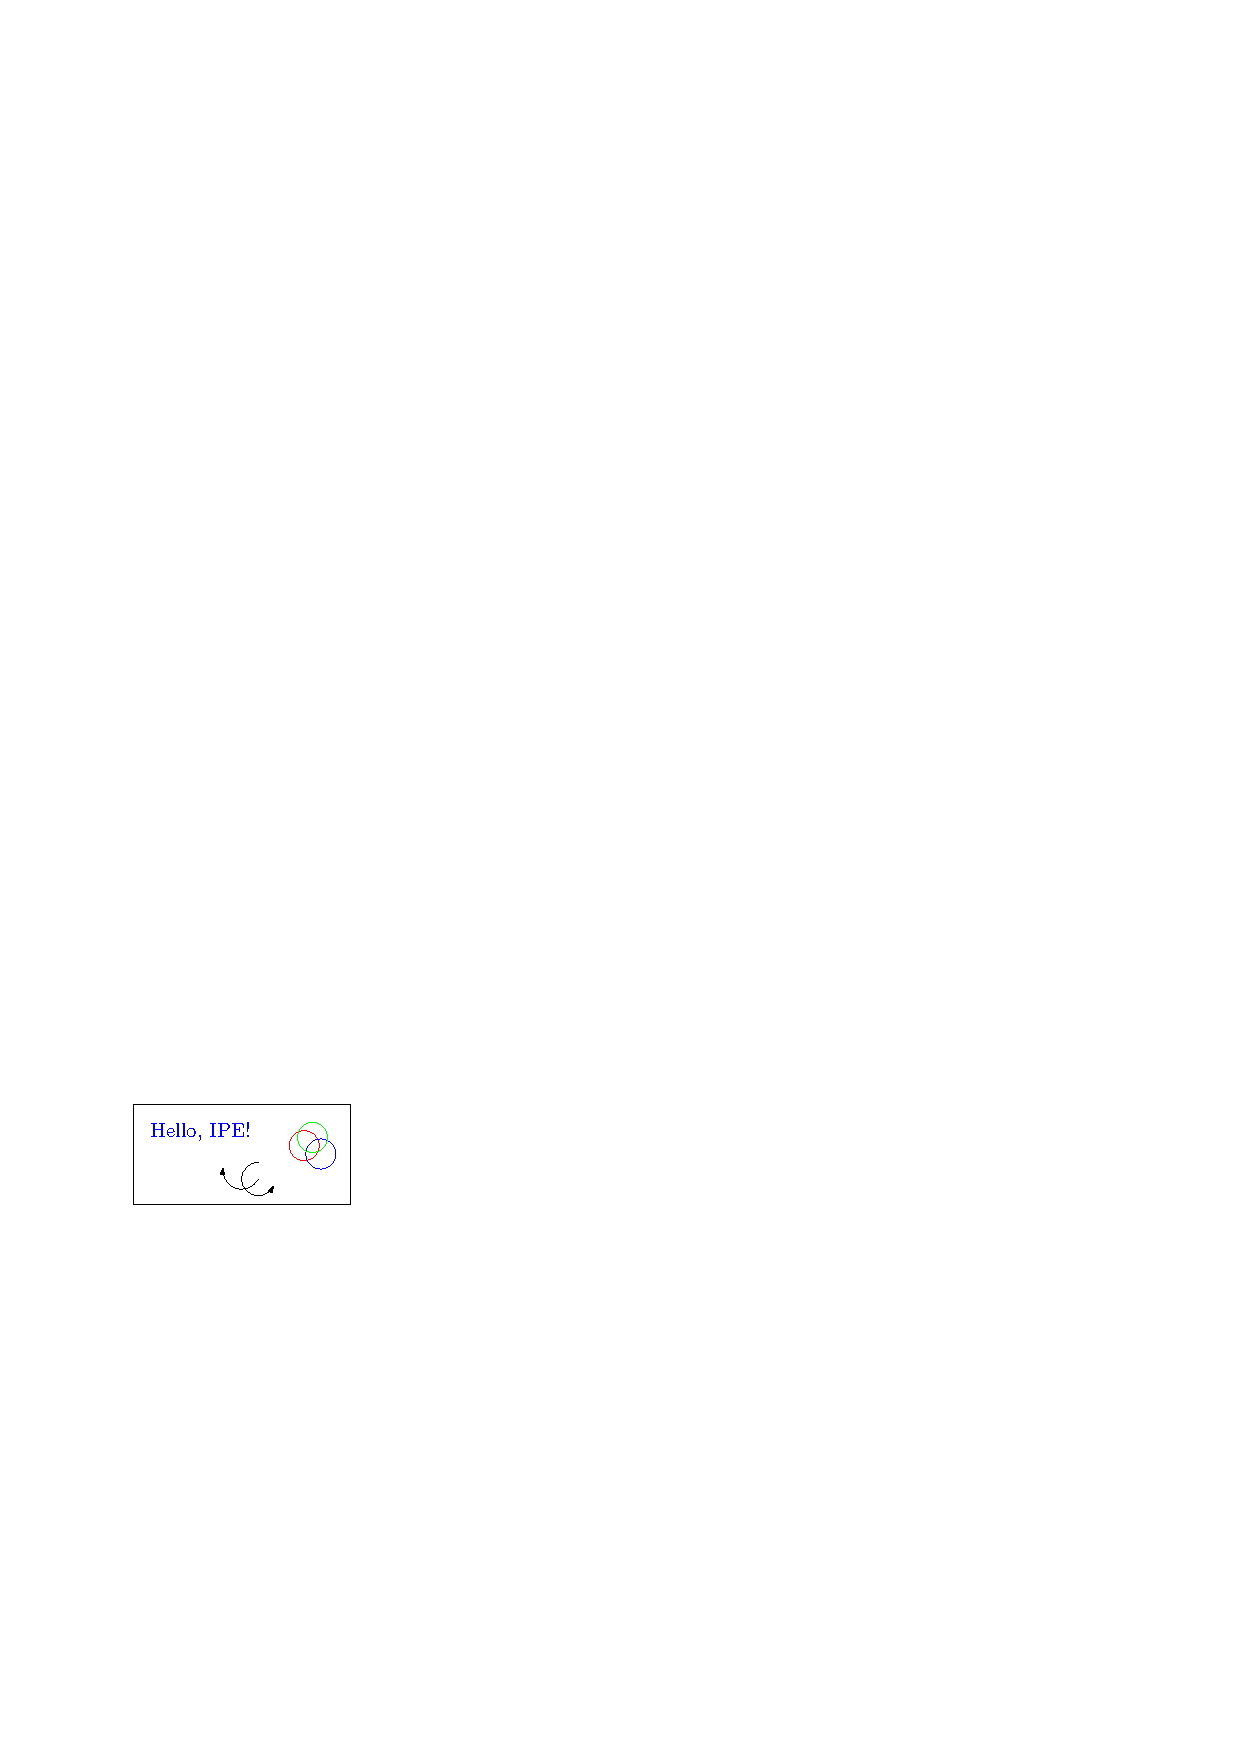
\includegraphics{hello}
  \caption*{图~1\hskip1em 这是手动编号但不出现索引中的图片的例子}
  \label{tab:badfigure3}    
\end{figure}

柳下季曰:“先生言为人父者必能诏其子,为人兄者必能教其弟,若子不听父之诏,弟不受
兄之教,虽今先生之辩,将奈之何哉?且跖之为人也,心如涌泉,意如飘风,强足以距敌,
辩足以饰非。顺其心则喜,逆其心则怒,易辱人以言。先生必无往。”

孔子不听,颜回为驭,子贡为右,往见盗跖。

\subsection*{整数规划}
盗跖乃方休卒徒大山之阳,脍人肝而餔之。孔子下车而前,见谒者曰:“鲁人孔丘,闻将军
高义,敬再拜谒者。”谒者入通。盗跖闻之大怒,目如明星,发上指冠,曰:“此夫鲁国之
巧伪人孔丘非邪?为我告之:尔作言造语,妄称文、武,冠枝木之冠,带死牛之胁,多辞缪
说,不耕而食,不织而衣,摇唇鼓舌,擅生是非,以迷天下之主,使天下学士不反其本,妄
作孝弟,而侥幸于封侯富贵者也。子之罪大极重,疾走归!不然,我将以子肝益昼餔之膳。”
%\end{annexS}%外文文献翻译
\end{document}
